\documentclass[officiallayout]{tktla} 
%\documentclass[officiallayout,a4frame]{tktla}
\usepackage[latin1]{inputenc}
\usepackage{microtype}
\usepackage{latexsym}
\usepackage{graphicx}

% my packages
\usepackage{natbib}
\bibpunct{(}{)}{;}{a}{,}{,}
\usepackage{bibentry}
\nobibliography*  
\usepackage{enumitem}
\usepackage[hidelinks]{hyperref}
\usepackage{physics}
\usepackage{cancel}
\usepackage{algorithm}
\usepackage[noend]{algpseudocode}
\usepackage{dsfont}
\usepackage{booktabs}
\usepackage{multirow}
\usepackage{subcaption}
\usepackage{xcolor}
\usepackage{arydshln}
\usepackage{tikz}[angles, quotes]
\usetikzlibrary{shapes.geometric}
\usepackage[most]{tcolorbox}
\usepackage{empheq}
\usepackage[export]{adjustbox}

\clubpenalty=10000
\widowpenalty=10000
\displaywidowpenalty=10000

%%%%% NEW MATH DEFINITIONS %%%%%

\usepackage{amsmath,amsfonts,bm,amsthm}

% Mark sections of captions for referring to divisions of figures
\newcommand{\figleft}{{\em (Left)}}
\newcommand{\figcenter}{{\em (Center)}}
\newcommand{\figright}{{\em (Right)}}
\newcommand{\figtop}{{\em (Top)}}
\newcommand{\figbottom}{{\em (Bottom)}}
\newcommand{\captiona}{{\em (a)}}
\newcommand{\captionb}{{\em (b)}}
\newcommand{\captionc}{{\em (c)}}
\newcommand{\captiond}{{\em (d)}}

% Highlight a newly defined term
\newcommand{\newterm}[1]{{\bf #1}}


% Figure reference, lower-case.
\def\figref#1{figure~\ref{#1}}
% Figure reference, capital. For start of sentence
\def\Figref#1{Figure~\ref{#1}}
\def\twofigref#1#2{figures \ref{#1} and \ref{#2}}
\def\quadfigref#1#2#3#4{figures \ref{#1}, \ref{#2}, \ref{#3} and \ref{#4}}
% Section reference, lower-case.
\def\secref#1{section~\ref{#1}}
% Section reference, capital.
\def\Secref#1{Section~\ref{#1}}
% Reference to two sections.
\def\twosecrefs#1#2{sections \ref{#1} and \ref{#2}}
% Reference to three sections.
\def\secrefs#1#2#3{sections \ref{#1}, \ref{#2} and \ref{#3}}
% Reference to an equation, lower-case.
% \def\eqref#1{equation~\ref{#1}}
% Reference to an equation, upper case
\def\Eqref#1{Equation~\ref{#1}}
% A raw reference to an equation---avoid using if possible
\def\plaineqref#1{\ref{#1}}
% Reference to a chapter, lower-case.
\def\chapref#1{chapter~\ref{#1}}
% Reference to an equation, upper case.
\def\Chapref#1{Chapter~\ref{#1}}
% Reference to a range of chapters
\def\rangechapref#1#2{chapters\ref{#1}--\ref{#2}}
% Reference to an algorithm, lower-case.
\def\algref#1{algorithm~\ref{#1}}
% Reference to an algorithm, upper case.
\def\Algref#1{Algorithm~\ref{#1}}
\def\twoalgref#1#2{algorithms \ref{#1} and \ref{#2}}
\def\Twoalgref#1#2{Algorithms \ref{#1} and \ref{#2}}
% Reference to a part, lower case
\def\partref#1{part~\ref{#1}}
% Reference to a part, upper case
\def\Partref#1{Part~\ref{#1}}
\def\twopartref#1#2{parts \ref{#1} and \ref{#2}}

\def\ceil#1{\lceil #1 \rceil}
\def\floor#1{\lfloor #1 \rfloor}
\def\1{\bm{1}}
\newcommand{\Dtrain}{\mathcal{D}}
\newcommand{\Dvalid}{\mathcal{D_{\mathrm{valid}}}}
\newcommand{\Dtest}{\mathcal{D_{\mathrm{test}}}}

\def\eps{{\epsilon}}


% Random variables
\def\reta{{\textnormal{$\eta$}}}
\def\ra{{\textnormal{a}}}
\def\rb{{\textnormal{b}}}
\def\rc{{\textnormal{c}}}
\def\rd{{\textnormal{d}}}
\def\re{{\textnormal{e}}}
\def\rf{{\textnormal{f}}}
\def\rg{{\textnormal{g}}}
\def\rh{{\textnormal{h}}}
\def\ri{{\textnormal{i}}}
\def\rj{{\textnormal{j}}}
\def\rk{{\textnormal{k}}}
\def\rl{{\textnormal{l}}}
% rm is already a command, just don't name any random variables m
\def\rn{{\textnormal{n}}}
\def\ro{{\textnormal{o}}}
\def\rp{{\textnormal{p}}}
\def\rq{{\textnormal{q}}}
\def\rr{{\textnormal{r}}}
\def\rs{{\textnormal{s}}}
\def\rt{{\textnormal{t}}}
\def\ru{{\textnormal{u}}}
\def\rv{{\textnormal{v}}}
\def\rw{{\textnormal{w}}}
\def\rx{{\textnormal{x}}}
\def\ry{{\textnormal{y}}}
\def\rz{{\textnormal{z}}}

% Random vectors
\def\rvepsilon{{\mathbf{\epsilon}}}
\def\rvtheta{{\mathbf{\theta}}}
\def\rva{{\mathbf{a}}}
\def\rvb{{\mathbf{b}}}
\def\rvc{{\mathbf{c}}}
\def\rvd{{\mathbf{d}}}
\def\rve{{\mathbf{e}}}
\def\rvf{{\mathbf{f}}}
\def\rvg{{\mathbf{g}}}
\def\rvh{{\mathbf{h}}}
\def\rvu{{\mathbf{i}}}
\def\rvj{{\mathbf{j}}}
\def\rvk{{\mathbf{k}}}
\def\rvl{{\mathbf{l}}}
\def\rvm{{\mathbf{m}}}
\def\rvn{{\mathbf{n}}}
\def\rvo{{\mathbf{o}}}
\def\rvp{{\mathbf{p}}}
\def\rvq{{\mathbf{q}}}
\def\rvr{{\mathbf{r}}}
\def\rvs{{\mathbf{s}}}
\def\rvt{{\mathbf{t}}}
\def\rvu{{\mathbf{u}}}
\def\rvv{{\mathbf{v}}}
\def\rvw{{\mathbf{w}}}
\def\rvx{{\mathbf{x}}}
\def\rvy{{\mathbf{y}}}
\def\rvz{{\mathbf{z}}}

% Elements of random vectors
\def\erva{{\textnormal{a}}}
\def\ervb{{\textnormal{b}}}
\def\ervc{{\textnormal{c}}}
\def\ervd{{\textnormal{d}}}
\def\erve{{\textnormal{e}}}
\def\ervf{{\textnormal{f}}}
\def\ervg{{\textnormal{g}}}
\def\ervh{{\textnormal{h}}}
\def\ervi{{\textnormal{i}}}
\def\ervj{{\textnormal{j}}}
\def\ervk{{\textnormal{k}}}
\def\ervl{{\textnormal{l}}}
\def\ervm{{\textnormal{m}}}
\def\ervn{{\textnormal{n}}}
\def\ervo{{\textnormal{o}}}
\def\ervp{{\textnormal{p}}}
\def\ervq{{\textnormal{q}}}
\def\ervr{{\textnormal{r}}}
\def\ervs{{\textnormal{s}}}
\def\ervt{{\textnormal{t}}}
\def\ervu{{\textnormal{u}}}
\def\ervv{{\textnormal{v}}}
\def\ervw{{\textnormal{w}}}
\def\ervx{{\textnormal{x}}}
\def\ervy{{\textnormal{y}}}
\def\ervz{{\textnormal{z}}}

% Random matrices
\def\rmA{{\mathbf{A}}}
\def\rmB{{\mathbf{B}}}
\def\rmC{{\mathbf{C}}}
\def\rmD{{\mathbf{D}}}
\def\rmE{{\mathbf{E}}}
\def\rmF{{\mathbf{F}}}
\def\rmG{{\mathbf{G}}}
\def\rmH{{\mathbf{H}}}
\def\rmI{{\mathbf{I}}}
\def\rmJ{{\mathbf{J}}}
\def\rmK{{\mathbf{K}}}
\def\rmL{{\mathbf{L}}}
\def\rmM{{\mathbf{M}}}
\def\rmN{{\mathbf{N}}}
\def\rmO{{\mathbf{O}}}
\def\rmP{{\mathbf{P}}}
\def\rmQ{{\mathbf{Q}}}
\def\rmR{{\mathbf{R}}}
\def\rmS{{\mathbf{S}}}
\def\rmT{{\mathbf{T}}}
\def\rmU{{\mathbf{U}}}
\def\rmV{{\mathbf{V}}}
\def\rmW{{\mathbf{W}}}
\def\rmX{{\mathbf{X}}}
\def\rmY{{\mathbf{Y}}}
\def\rmZ{{\mathbf{Z}}}

% Elements of random matrices
\def\ermA{{\textnormal{A}}}
\def\ermB{{\textnormal{B}}}
\def\ermC{{\textnormal{C}}}
\def\ermD{{\textnormal{D}}}
\def\ermE{{\textnormal{E}}}
\def\ermF{{\textnormal{F}}}
\def\ermG{{\textnormal{G}}}
\def\ermH{{\textnormal{H}}}
\def\ermI{{\textnormal{I}}}
\def\ermJ{{\textnormal{J}}}
\def\ermK{{\textnormal{K}}}
\def\ermL{{\textnormal{L}}}
\def\ermM{{\textnormal{M}}}
\def\ermN{{\textnormal{N}}}
\def\ermO{{\textnormal{O}}}
\def\ermP{{\textnormal{P}}}
\def\ermQ{{\textnormal{Q}}}
\def\ermR{{\textnormal{R}}}
\def\ermS{{\textnormal{S}}}
\def\ermT{{\textnormal{T}}}
\def\ermU{{\textnormal{U}}}
\def\ermV{{\textnormal{V}}}
\def\ermW{{\textnormal{W}}}
\def\ermX{{\textnormal{X}}}
\def\ermY{{\textnormal{Y}}}
\def\ermZ{{\textnormal{Z}}}

% Vectors
\def\vzero{{\bm{0}}}
\def\vone{{\bm{1}}}
\def\vmu{{\bm{\mu}}}
\def\vtheta{{\bm{\theta}}}
\def\va{{\bm{a}}}
\def\vb{{\bm{b}}}
\def\vc{{\bm{c}}}
\def\vd{{\bm{d}}}
\def\ve{{\bm{e}}}
\def\vf{{\bm{f}}}
\def\vg{{\bm{g}}}
\def\vh{{\bm{h}}}
\def\vi{{\bm{i}}}
\def\vj{{\bm{j}}}
\def\vk{{\bm{k}}}
\def\vl{{\bm{l}}}
\def\vm{{\bm{m}}}
\def\vn{{\bm{n}}}
\def\vo{{\bm{o}}}
\def\vp{{\bm{p}}}
\def\vq{{\bm{q}}}
\def\vr{{\bm{r}}}
\def\vs{{\bm{s}}}
\def\vt{{\bm{t}}}
\def\vu{{\bm{u}}}
\def\vv{{\bm{v}}}
\def\vw{{\bm{w}}}
\def\vx{{\bm{x}}}
\def\vy{{\bm{y}}}
\def\vz{{\bm{z}}}

% Elements of vectors
\def\evalpha{{\alpha}}
\def\evbeta{{\beta}}
\def\evepsilon{{\epsilon}}
\def\evlambda{{\lambda}}
\def\evomega{{\omega}}
\def\evmu{{\mu}}
\def\evpsi{{\psi}}
\def\evsigma{{\sigma}}
\def\evtheta{{\theta}}
\def\eva{{a}}
\def\evb{{b}}
\def\evc{{c}}
\def\evd{{d}}
\def\eve{{e}}
\def\evf{{f}}
\def\evg{{g}}
\def\evh{{h}}
\def\evi{{i}}
\def\evj{{j}}
\def\evk{{k}}
\def\evl{{l}}
\def\evm{{m}}
\def\evn{{n}}
\def\evo{{o}}
\def\evp{{p}}
\def\evq{{q}}
\def\evr{{r}}
\def\evs{{s}}
\def\evt{{t}}
\def\evu{{u}}
\def\evv{{v}}
\def\evw{{w}}
\def\evx{{x}}
\def\evy{{y}}
\def\evz{{z}}

% Matrix
\def\mA{{\bm{A}}}
\def\mB{{\bm{B}}}
\def\mC{{\bm{C}}}
\def\mD{{\bm{D}}}
\def\mE{{\bm{E}}}
\def\mF{{\bm{F}}}
\def\mG{{\bm{G}}}
\def\mH{{\bm{H}}}
\def\mI{{\bm{I}}}
\def\mJ{{\bm{J}}}
\def\mK{{\bm{K}}}
\def\mL{{\bm{L}}}
\def\mM{{\bm{M}}}
\def\mN{{\bm{N}}}
\def\mO{{\bm{O}}}
\def\mP{{\bm{P}}}
\def\mQ{{\bm{Q}}}
\def\mR{{\bm{R}}}
\def\mS{{\bm{S}}}
\def\mT{{\bm{T}}}
\def\mU{{\bm{U}}}
\def\mV{{\bm{V}}}
\def\mW{{\bm{W}}}
\def\mX{{\bm{X}}}
\def\mY{{\bm{Y}}}
\def\mZ{{\bm{Z}}}
\def\mBeta{{\bm{\beta}}}
\def\mPhi{{\bm{\Phi}}}
\def\mLambda{{\bm{\Lambda}}}
\def\mSigma{{\bm{\Sigma}}}

% Tensor
\DeclareMathAlphabet{\mathsfit}{\encodingdefault}{\sfdefault}{m}{sl}
\SetMathAlphabet{\mathsfit}{bold}{\encodingdefault}{\sfdefault}{bx}{n}
\newcommand{\tens}[1]{\bm{\mathsfit{#1}}}
\def\tA{{\tens{A}}}
\def\tB{{\tens{B}}}
\def\tC{{\tens{C}}}
\def\tD{{\tens{D}}}
\def\tE{{\tens{E}}}
\def\tF{{\tens{F}}}
\def\tG{{\tens{G}}}
\def\tH{{\tens{H}}}
\def\tI{{\tens{I}}}
\def\tJ{{\tens{J}}}
\def\tK{{\tens{K}}}
\def\tL{{\tens{L}}}
\def\tM{{\tens{M}}}
\def\tN{{\tens{N}}}
\def\tO{{\tens{O}}}
\def\tP{{\tens{P}}}
\def\tQ{{\tens{Q}}}
\def\tR{{\tens{R}}}
\def\tS{{\tens{S}}}
\def\tT{{\tens{T}}}
\def\tU{{\tens{U}}}
\def\tV{{\tens{V}}}
\def\tW{{\tens{W}}}
\def\tX{{\tens{X}}}
\def\tY{{\tens{Y}}}
\def\tZ{{\tens{Z}}}


% Graph
\def\gA{{\mathcal{A}}}
\def\gB{{\mathcal{B}}}
\def\gC{{\mathcal{C}}}
\def\gD{{\mathcal{D}}}
\def\gE{{\mathcal{E}}}
\def\gF{{\mathcal{F}}}
\def\gG{{\mathcal{G}}}
\def\gH{{\mathcal{H}}}
\def\gI{{\mathcal{I}}}
\def\gJ{{\mathcal{J}}}
\def\gK{{\mathcal{K}}}
\def\gL{{\mathcal{L}}}
\def\gM{{\mathcal{M}}}
\def\gN{{\mathcal{N}}}
\def\gO{{\mathcal{O}}}
\def\gP{{\mathcal{P}}}
\def\gQ{{\mathcal{Q}}}
\def\gR{{\mathcal{R}}}
\def\gS{{\mathcal{S}}}
\def\gT{{\mathcal{T}}}
\def\gU{{\mathcal{U}}}
\def\gV{{\mathcal{V}}}
\def\gW{{\mathcal{W}}}
\def\gX{{\mathcal{X}}}
\def\gY{{\mathcal{Y}}}
\def\gZ{{\mathcal{Z}}}

% Sets
\def\sA{{\mathbb{A}}}
\def\sB{{\mathbb{B}}}
\def\sC{{\mathbb{C}}}
\def\sD{{\mathbb{D}}}
% Don't use a set called E, because this would be the same as our symbol
% for expectation.
\def\sF{{\mathbb{F}}}
\def\sG{{\mathbb{G}}}
\def\sH{{\mathbb{H}}}
\def\sI{{\mathbb{I}}}
\def\sJ{{\mathbb{J}}}
\def\sK{{\mathbb{K}}}
\def\sL{{\mathbb{L}}}
\def\sM{{\mathbb{M}}}
\def\sN{{\mathbb{N}}}
\def\sO{{\mathbb{O}}}
\def\sP{{\mathbb{P}}}
\def\sQ{{\mathbb{Q}}}
\def\sR{{\mathbb{R}}}
\def\sS{{\mathbb{S}}}
\def\sT{{\mathbb{T}}}
\def\sU{{\mathbb{U}}}
\def\sV{{\mathbb{V}}}
\def\sW{{\mathbb{W}}}
\def\sX{{\mathbb{X}}}
\def\sY{{\mathbb{Y}}}
\def\sZ{{\mathbb{Z}}}

% Entries of a matrix
\def\emLambda{{\Lambda}}
\def\emA{{A}}
\def\emB{{B}}
\def\emC{{C}}
\def\emD{{D}}
\def\emE{{E}}
\def\emF{{F}}
\def\emG{{G}}
\def\emH{{H}}
\def\emI{{I}}
\def\emJ{{J}}
\def\emK{{K}}
\def\emL{{L}}
\def\emM{{M}}
\def\emN{{N}}
\def\emO{{O}}
\def\emP{{P}}
\def\emQ{{Q}}
\def\emR{{R}}
\def\emS{{S}}
\def\emT{{T}}
\def\emU{{U}}
\def\emV{{V}}
\def\emW{{W}}
\def\emX{{X}}
\def\emY{{Y}}
\def\emZ{{Z}}
\def\emSigma{{\Sigma}}

% entries of a tensor
% Same font as tensor, without \bm wrapper
\newcommand{\etens}[1]{\mathsfit{#1}}
\def\etLambda{{\etens{\Lambda}}}
\def\etA{{\etens{A}}}
\def\etB{{\etens{B}}}
\def\etC{{\etens{C}}}
\def\etD{{\etens{D}}}
\def\etE{{\etens{E}}}
\def\etF{{\etens{F}}}
\def\etG{{\etens{G}}}
\def\etH{{\etens{H}}}
\def\etI{{\etens{I}}}
\def\etJ{{\etens{J}}}
\def\etK{{\etens{K}}}
\def\etL{{\etens{L}}}
\def\etM{{\etens{M}}}
\def\etN{{\etens{N}}}
\def\etO{{\etens{O}}}
\def\etP{{\etens{P}}}
\def\etQ{{\etens{Q}}}
\def\etR{{\etens{R}}}
\def\etS{{\etens{S}}}
\def\etT{{\etens{T}}}
\def\etU{{\etens{U}}}
\def\etV{{\etens{V}}}
\def\etW{{\etens{W}}}
\def\etX{{\etens{X}}}
\def\etY{{\etens{Y}}}
\def\etZ{{\etens{Z}}}

% The true underlying data generating distribution
\newcommand{\pdata}{p_{\rm{data}}}
% The empirical distribution defined by the training set
\newcommand{\ptrain}{\hat{p}_{\rm{data}}}
\newcommand{\Ptrain}{\hat{P}_{\rm{data}}}
% The model distribution
\newcommand{\pmodel}{p_{\rm{model}}}
\newcommand{\Pmodel}{P_{\rm{model}}}
\newcommand{\ptildemodel}{\tilde{p}_{\rm{model}}}
% Stochastic autoencoder distributions
\newcommand{\pencode}{p_{\rm{encoder}}}
\newcommand{\pdecode}{p_{\rm{decoder}}}
\newcommand{\precons}{p_{\rm{reconstruct}}}

\newcommand{\laplace}{\mathrm{Laplace}} % Laplace distribution

\newcommand{\E}{\mathbb{E}}
\newcommand{\Ls}{\mathcal{L}}
\newcommand{\R}{\mathbb{R}}
\newcommand{\emp}{\tilde{p}}
\newcommand{\lr}{\alpha}
\newcommand{\reg}{\lambda}
\newcommand{\rect}{\mathrm{rectifier}}
\newcommand{\softmax}{\mathrm{softmax}}
\newcommand{\sigmoid}{\sigma}
\newcommand{\softplus}{\zeta}
\newcommand{\KL}{D_{\mathrm{KL}}}
\newcommand{\Var}{\mathrm{Var}}
\newcommand{\standarderror}{\mathrm{SE}}
\newcommand{\Cov}{\mathrm{Cov}}
% Wolfram Mathworld says $L^2$ is for function spaces and $\ell^2$ is for vectors
% But then they seem to use $L^2$ for vectors throughout the site, and so does
% wikipedia.
\newcommand{\normlzero}{L^0}
\newcommand{\normlone}{L^1}
\newcommand{\normltwo}{L^2}
\newcommand{\normlp}{L^p}
\newcommand{\normmax}{L^\infty}

\newcommand{\parents}{Pa} % See usage in notation.tex. Chosen to match Daphne's book.

\DeclareMathOperator*{\argmax}{arg\,max}
\DeclareMathOperator*{\argmin}{arg\,min}

\DeclareMathOperator{\sign}{sign}
% \DeclareMathOperator{\Tr}{Tr}
\let\ab\allowbreak

% My commands
\newcommand{\inp}[2]{\left\langle #1, #2 \right\rangle}



\newtheorem{theorem}{Theorem}[chapter]
\newtheorem{proposition}{Proposition}
\newtheorem{lemma}{Lemma}
\newtheorem{observation}{Observation}
 


\tcbset{
  thesisstatement/.style={
    colback=gray!10,     % background color
      colframe=black!60,   % border color
      arc=4pt,             % rounded corners
      boxrule=0.8pt,       % border thickness
      left=6pt, right=6pt, top=6pt, bottom=6pt
  }
}



\tcolorboxenvironment{theorem}{thesisstatement}
\tcolorboxenvironment{proposition}{thesisstatement}
\tcolorboxenvironment{observation}{thesisstatement}
\tcolorboxenvironment{lemma}{thesisstatement}


\definecolor{mycolor}{RGB}{180, 40, 40}



\title{Geometric Methods for Bayesian Inference and Modeling Discrete Data}
\author{Bernardo Williams}
\authorcontact{bernardo.williamsmoreno@helsinki.fi
% \par http://cs.helsinki.fi/John.Smith/
}
\pubtime{September}{2026}
\reportno{15}
% ISBN 978-952-84-3244-9 (softcover)
% ISBN 978-952-84-3245-6 (PDF)
\isbnpaperback{978-952-84-3244-9}
\isbnpdf{978-952-84-3245-6}
\issn{1238-8645}
\issnonline{2814-4031}
\printhouse{Unigrafia}
\pubpages{73 + 99} % --- remember to update this! 
% For monographs, the number of the last page of the list of references
% For article-based theses, the number of the last page of the list of
% references of the preamble part + the total number of the pages of
% the original articles and interleaf pages.
\supervisorlist{
Arto Klami, University of Helsinki, Finland \\
$\hspace{1.0em}$ Marcelo Hartmann, University of Helsinki, Finland
}


\preexaminera{Martin Trapp, KTH Royal Institute of Technology, Sweden}
\preexaminerb{Alice Le Brigant, University Paris 1 Pantheon Sorbonne, France }
\opponent{Martin Trapp, KTH Royal Institute of Technology, Sweden}
\custos{Arto Klami, University of Helsinki, Finland}
\generalterms{Machine learning, Bayesian inference, generative models}
\additionalkeywords{Laplace approximation, Markov chain Monte Carlo, flow models, Gaussian process}


\crclong{
\item Mathematics of computing $\rightarrow$ Probability and statistics $\rightarrow$ Probabilistic inference problems $\rightarrow$ Bayesian computation
\item Computing methodologies $\rightarrow$ Machine learning $\rightarrow$ Learning paradigms $\rightarrow$ Supervised learning
}

\permissionnotice{
  Doctoral dissertation, to be presented for public examination with 
  the permission of the Faculty of Science of the University of
  Helsinki in Auditorium E204, Physicum, on September 18 at 13:00. 
}



\begin{document}

\frontmatter

\maketitle

\begin{abstract}
  
This thesis studies how geometry can be used to improve methods for approximate Bayesian inference and modeling discrete data. 
% 
In both cases the relevant statistical object is non-Euclidean. In Bayesian inference the parameters of a distribution family can be viewed as a statistical manifold. In discrete data modeling, probability vectors are in the simplex, a compact space with own geometric structure. This thesis asks the question: when does geometry-aware modeling leads to more accurate, and in some cases, simpler methods?   
% 
It also explores what computational tradeoffs such approaches might introduce. 


The first part studies Bayesian inference, the task of approximating a posterior distribution. We consider Riemannian Laplace approximation and geometric Markov chain Monte Carlo methods for posterior distributions with strong curvature and multimodality. We show that geometry-aware methods improves the sample quality, but the metric must be chosen carefully. Metrics that better capture the geometry of the target space tend to be more accurate, while computationally efficient alternatives improve scalability at the cost of reduced accuracy. 

The second part studies discrete data modeling, through inference of distributions on the probability simplex. We develop methods that rely on simplex-to-Euclidean bijections and stochastic interpolations. These bijections map the discrete data to continuous unbounded latent representations, while the interpolations allow for faithful recovery of the original categories. This construction allows the use of Euclidean tools for generative modeling and classification. In particular we develop simplex-to-Euclidean flow matching for discrete data generation and a multiclass Gaussian Process classifier that has exact latent variable inference. 

Throughout the thesis the main finding is that geometry-aware modeling can improve statistical performance. In Bayesian inference it gives accurate samples in curved and multimodal distributions, and in discrete data modeling, it reformulates the problem by connecting to latent continuous representations.   

\end{abstract}

\begin{acknowledgements}

I would like to begin by thanking my supervisors, Arto and Marcelo, for taking me in as their student and for their constant support and guidance over the years.
They gave me room to explore ideas, be creative, and sharpen the skills that shape me as a researcher. I am especially grateful for their on-point, thoughtful comments that have helped me improve my work through the course of many iterations.
Their support was extended beyond research to matters adjacent to work, in which they showed humanism, professionalism and empathy.
I am also thankful to the pre-examiners of this thesis, Alice Le Brigant and Martin Trapp, for the time taken to read the work and for providing detailed comments. I am especially grateful to Martin for serving as my opponent. 

I have been privileged enough to turn my passion into a profession over the last four years. This was made possible by the funding provided by the Research Council of Finland through the projects ``Efficient Riemannian Inference'' and ``Flexible priors for flexible models'', in which I was included by my supervisors. 
Not only did these projects fund my salary, but they also allowed me to present our papers at conferences on four different continents. 
I gratefully acknowledge the UnaEuropa grant that supported my visit to the University of Edinburgh, and extend my gratitude to Viacheslav Borovitskiy for the warm welcome and for hosting me during a fruitful research visit. 

I have been fortunate to be surrounded by talented and hardworking people and the collaborations it has led to. My publications have greatly benefited from my coauthors. 
I am appreciative of the  Multi-source probabilistic inference group, and of our subgroup, the ``Monge'' group, which provided a consistent place to present ideas, have interesting discussions, and give and receive feedback. 
I am grateful to Cosmo, Hanlin, Shayan and Ville for our paper discussion forum (PDF); our shared journey made the PhD path more pleasant and more productive.
Additionally, I would like to express my gratitude to Ali Amiryousefi who introduced me to research in the first place.

I am grateful to the University of Helsinki for many reasons.
It provided off-work activities to the doctoral students that made it a great place to work.
It offered language courses and language events that allowed me to dive deeply into the culture of this country in a safe space and in an enjoyable way.
Special thanks go to P\"aivi Vetsch and Daniel Radice, who played an important role in this matter.


Finally I would like to thank my parents. Your unconditional and lifelong support has allowed me to reside in different parts of the world, and let me pursue work that fulfills me.
I am grateful beyond words.
And to my partner, Elenia, who has given me unconditional love and support at each step of the journey, I am forever grateful. 


  
\begin{flushright}
  Helsinki, September 2026\\
  Bernardo Williams
\end{flushright}
\end{acknowledgements}

\tableofcontents
\chapter*{List of Publications}

This thesis is based on the following four original articles, referred throughout as Papers I-IV. The full articles are appended at the end of the thesis.
\begin{enumerate}[label=\textbf{\Roman*:}]
    \item \bibentry{yu2024riemannian}
    \item \bibentry{williams2025geodesic}
    \item \bibentry{Williams2026}
    \item \bibentry{williams2026simplex}
\end{enumerate}

\newpage

\section*{Author Contributions}

\paragraph{Publication I: ``Riemannian Laplace Approximation with the Fisher Metric"}
HY conceived the idea, wrote the code of the experiments and wrote the first draft of the manuscript. MH proposed the use of the Fisher-Rao metric in Riemann-Laplace method, and helped writing the theoretical derivations of central concepts in the paper. BW contributed to the code implementation. All authors jointly participated in the  discussions and in the writing of the manuscript. 

\paragraph{Publication II: ``Geodesic Slice Sampler for Multimodal Distributions with Strong Curvature"}
BW conceived the idea, wrote the code of the experiments, ran all the experiments, and wrote the first draft of the manuscript. The theoretical analysis was  initially done by BW and corrected and improved  with help from HY, HPHL and MH. The writing of the paper was done as joint collaboration of all authors, with AK and MH providing supervision and guidance through the whole process. MH additionally introduced external collaboration for BW, which benefited paper writing and development: GA suggested the teaser image and changes to text. 

\paragraph{Publication III:``Simplex-to-Euclidean bijections for Categorical Flow Matching"}
BW conceived the paper's idea, wrote the code of the experiments and wrote the first draft of the manuscript. 
BW executed all of the experiments and derived the theoretical results. VYS implemented  the comparison methods (SEDD) and measured running times of the methods (App. C.3). Jointly all authors participated in the discussion and writing of the paper.


\paragraph{Publication IV:``Simplex-to-Euclidean Bijection for Conjugate and Calibrated Multiclass Gaussian Process Classification"}
BW and MH jointly conceived the paper's original idea. BW wrote the code of the experiments, wrote the first draft of the manuscript, and derived the theoretical results. HT and MH proof read the propositions and theorems. All of the authors  participated in the discussion and writing.  

\chapter*{Notation}
\markboth{Notation}{Notation}
These tables collect the most important notation and are organized by topic. 

\paragraph{Geometric Bayesian inference}
\begin{center}
\renewcommand{\arraystretch}{1.15}
\begin{tabular}{p{0.28\textwidth}p{0.68\textwidth}}
$\boldsymbol{x}\in\mathbb{R}^{D}$, $p(\boldsymbol{x})$,  & Variable of interest and target density. \\
$\ell(\boldsymbol{x}):=\log p(\boldsymbol{x})$ & Log-target density.\\
$\hat{\boldsymbol{x}}$ & Mode or MAP estimate of the target. \\
$\mathbf{G}(\boldsymbol{x})$ & Riemannian metric tensor. \\
$\operatorname{Exp}_{\boldsymbol{x}}$, $\operatorname{Log}_{\boldsymbol{x}}$ & Exponential and logarithm maps induced by the metric. \\
$\gamma_{\boldsymbol{x}, \boldsymbol{v}}(t)$ & Geodesic at time $t$ with initial conditions $\boldsymbol{x}, \boldsymbol{v}$. \\
$p_{\mathcal{H}}(\boldsymbol{x})$ & Hausdorff density associated with the Riemannian volume. \\
$\Gamma^k_{ij}(\boldsymbol{x})$ & Christoffel symbols of the second kind. \\
\end{tabular}
\end{center}

\paragraph{Gaussian Processes}
\begin{center}
\renewcommand{\arraystretch}{1.15}
\begin{tabular}{p{0.28\textwidth}p{0.68\textwidth}}
$\mathbf{f}(\cdot)\sim\mathcal{GP}(\mathbf{0},K_{\theta})$ & Latent Gaussian process prior with zero mean and kernel $K_{\theta}$. \\
$\boldsymbol{\mu}_*$, $\boldsymbol{\Sigma}_*$ &  predictive mean, and predictive covariance in the GP model for point $\boldsymbol{x}_*$. \\
$\sigma^2$ & Latent Gaussian noise variance. \\
\end{tabular}
\end{center}

\newpage
\paragraph{Latent constructions}
\begin{center}
\renewcommand{\arraystretch}{1.15}
\begin{tabular}{p{0.28\textwidth}p{0.68\textwidth}}
$K$, $D:=K-1$ & Number of categories and corresponding latent dimension. \\
$c_i, \boldsymbol{x}_i, \boldsymbol{z}_i$, $\boldsymbol{r}_i$ & Class label $c_i\in \{1,..,K\}$, point in open simplex, point in Euclidean space and regressor. \\
$\Delta^{D}$, $\mathring{\Delta}^{D}$ & Closed simplex and open simplex. \\
$\varphi$, $\varphi^{-1}$ & Bijection between the open simplex and Euclidean latent space. \\
$\langle\cdot,\cdot\rangle_A$, $d_A(\cdot,\cdot)$ & Aitchison inner product and Aitchison distance on the simplex. \\
$\mathcal{R}_k$ & Strict $\arg\max$ region associated with category $k$. \\
$\boldsymbol{\pi}$, $\hat{\boldsymbol{\pi}}$ & True and estimated categorical probabilities. \\
$\lambda$, $\alpha$ & Interpolation weight and Dirichlet noise parameter. \\
$\boldsymbol{\mu}^{(k)}$, $\boldsymbol{m}^{(k)}=\varphi(\boldsymbol{\mu}^{(k)})$ & Simplex and latent Euclidean representatives of class $k$. \\
$p_0,p_1,p_t$ & Base distribution, data distribution, and marginal distribution at time $t$. \\
$\boldsymbol{u}_t(\cdot|\boldsymbol{z})$, $\boldsymbol{v}_t^{\theta}(\cdot)$ & Target conditional velocity field and parametric velocity field.  
\end{tabular}
\end{center}
∑

\mainmatter

\chapter{Introduction}
This thesis studies geometric methods for two core tasks in machine learning: Bayesian inference and discrete data modeling.  In both cases we start with a probabilistic model whose unknown parameters are to be estimated in a principled way. In Bayesian inference \citep{gelman1995bayesian}, knowledge is given as a prior distribution, which  is updated with the observed data, resulting in a posterior distribution through Bayes' rule. 
% 
In a few special cases (such as classic Gaussian process regression) the posterior distribution belongs to the same probability distribution family as the prior. 
% 
This prior-likelihood model combination is called conjugate. In this case, posterior inference reduces to computing the parameters of the posterior distribution, and if the distribution family allows it, we can directly generate samples. 
% 
However, for most models the posterior distribution is not available in conjugate form, and we rely on approximate inference techniques to approximate the distribution or to draw samples from it. 


Recently, machine learning places emphasis on generative modeling, where the objective is to use the available data  to estimate the unknown parameters and then draw new  samples from the fitted model. This process is applied for example to create images, videos, molecules or text \citep{lipman2024flowmatchingguidecode}. A common technique is modeling the transport map from a simple base distribution (e.g. Gaussian) to the data distribution \citep{Albergo2023,Lipman2023,liu2023flow}. Generation is then performed by sampling from the simple base distribution and transporting those samples to the empirical data distribution using the learned model. This strategy is naturally defined for continuous data, but it can also be applied to discrete data through continuous relaxations, provided we have a reliable way to map generated points back to discrete outcomes.


This thesis studies a common theme: geometry \citep{amari2000methods,Lee2018}. 
In both approximate Bayesian inference and discrete data modeling, our constructed methods  measure distances and follow trajectories in a space determined by the underlying statistical object. 
Often there is no attention to the geometry, and Euclidean geometry is assumed by convention. Posterior distributions can have strong local curvature \citep{Girolami2011} or multiple separated modes \citep{Lan2014}. Discrete probability vectors lie on the simplex, which has its own intrinsic geometry \citep{Aitchison1986}. Ignoring this structure often leads to methods that are simple but inaccurate.

Riemannian geometry \citep{do1992riemannian,Lee2018} provides tools to encode local structure through a metric and to build algorithms that adhere to it. The metric choice introduces a tradeoff: richer geometry can improve statistical behavior while often increasing the computational cost, since even a simple operation like measuring the distance between two points may now require integration. For practical methods, geometry must therefore be chosen not only for faithfulness to the target distribution, but also for computational efficiency and tractability. 

In Bayesian inference, let us consider the problem of sampling from curved unimodal posterior distributions. \citet{Girolami2011} proposed adapting to the posterior geometry by using the Fisher information metric, which captures local structure from the Kullback-Leibler divergence. The problem is that the metric is expensive to compute, is problem specific, and is intractable for some distributions. Alternatively, metrics based on the geometry of the posterior graph \citep{Hartmann2022, hartmann:2023} can be computationally cheaper but are not completely faithful to the underlying geometry. Paper~I studies the balance between these two metric choices. An adjacent problem is multimodal sampling. While geometry-aware samplers can improve exploration of strongly curved targets, their application to multimodal targets is less developed than tempering and diffusion based variants \citep{Lan2014, Latuszynski2025}. Paper~II offers a new sampling strategy and metric choice for curved and multimodal targets. In Bayesian inference, the choice of metric is a modeling decision (curved and/or multimodal) and a computational one. 

In discrete data modeling, geometry naturally arises \citep{fisher1925theory, Aitchison1986}. The simplex is a compact convex subset of $\mathbb{R}^{K}$  defined by non-negative components that sum up to one. This space can be given the Fisher information geometry of the categorical distribution, but this approach implicitly models distributions on a compact space. Since much work has been done on Euclidean space, a bijection that respects the geometry of the simplex and connects to Euclidean space eases modeling. The log-ratio geometry between the elements is known as Aitchison geometry and provides simplex-to-Euclidean bijections. These maps allow for generative modeling and classification in the simplex via a latent Euclidean representation. We develop stochastic interpolations that convert discrete data to open simplex distributions, since the bijections are defined on the interior. In Bayesian classification the posterior distribution is usually intractable, but the bijections with the stochastic interpolation make it possible to fit a conjugate model in the latent space. Papers~III and~IV focus on generative modeling and classification respectively. 

\section*{Research questions} 
The following questions summarize the high level themes of the thesis:
\begin{enumerate}
    \item How can the geometric structure of the target density be used to improve approximate Bayesian inference?
    \item How can geometry-aware sampling methods better handle targets with both strong curvature and multimodality?
    \item How can the simplex geometry be connected to Euclidean representations for modeling discrete data?
    \item Can the Aitchison geometry enable simpler and exact inference procedures in multiclass classification?
\end{enumerate}


The aim of the thesis is to advance geometric methods both in the context of approximate Bayesian inference and modeling discrete data, by developing methods that use geometry in novel ways. Concretely, the Bayesian inference part studies geometry-aware posterior approximation and sampling through Riemannian Laplace approximation (Paper I) and geodesic slice sampling (Paper~II). The discrete-modeling part studies simplex-to-Euclidean bijections and stochastic interpolations for discrete data generation (Paper~III) and conjugate Gaussian process classification (Paper IV).


The thesis is organized as follows. Chapter~\ref{ch:background} provides the background on  Riemannian geometry, approximate Bayesian inference and modeling discrete data that our contributions build on. 
The core content is then divided into two main blocks. 
The first block (Chapter~\ref{ch:mcmc}) focuses on Bayesian inference, studying geometric improvements for posterior approximation and sampling. The second block (Chapter~\ref{ch:simplex}) focuses on modeling discrete data, using the simplex geometry to build methods that connect naturally to Euclidean tools. Across both parts, the main objective is the same: efficient geometric modeling that improves statistical performance.


\section*{Summary of the contributions} 
This thesis makes the following methodological contributions:
\begin{itemize}
    \item The thesis proposes modifying the choice of the Riemannian metric tensor in two Bayesian inference methods: Riemannian Laplace approximation ({Paper I}) and geodesic slice sampler ({Paper II}).
    \item  The Riemannian Laplace approximation with the Monge metric has an inherent bias on Gaussian targets. {Paper I} proposes two techniques to correct the bias: (i) using the logarithm map, and (ii) using the Fisher information as the metric tensor.
    \item {Paper II} adapts the geodesic slice sampler, which was previously used for manifolds with closed form geodesics, to target distributions defined on Euclidean space.  It also proposes new Riemannian metrics constructed from the target density for multimodal sampling. 
    \item The thesis proposes using simplex-to-Euclidean bijections and stochastic interpolations for modeling discrete data in Euclidean space instead of the simplex. Two different problems are studied: discrete data generation ({Paper III}) and  Gaussian process classification ({Paper IV}).     
    \item Based on the Euclidean representations, the thesis proposes using general purpose latent Euclidean models for discrete data, including flow-based generative models (Paper III) and Gaussian process regression models for classification (Paper IV).
    \end{itemize}

\chapter{Background} \label{ch:background}



This chapter introduces the background needed for the methods developed in Chapters~\ref{ch:mcmc} and \ref{ch:simplex}.  We start by giving a brief introduction to Riemannian geometry, then introducing methods for approximate Bayesian inference and finally approaches for modeling discrete data. 

\section{Basic notions in Riemannian Geometry} \label{sec:riemannian_background}
For a formal and rigorous introduction to Riemannian geometry we refer the reader to \citet{do1992riemannian} and \citet{Lee2018}. Here we introduce only the concepts needed later in the thesis, under simplified settings that cover our examples. We consider manifolds that admit a global chart, a subset of which are  smooth embedded submanifolds of Euclidean space. This allows us to write the coordinates globally, and avoid dealing with local coordinates patches. When the space has a boundary (e.g. the simplex) we consider the differential geometric objects only on the interior of the space. 

\subsection{Riemannian manifolds}

\paragraph{Manifolds and tangent spaces}
A smooth $D$-dimensional manifold $\mathcal{M}$ is a topological space that is
locally diffeomorphic to $\mathbb{R}^D$. For the manifolds we consider, we assume that
$\mathcal{M}$ admits a global chart $\varphi:\mathcal{M}\to U\subseteq\mathbb{R}^D$
with inverse $\psi=\varphi^{-1}$. For $\boldsymbol{x} \in \mathcal{M}$, we denote its coordinates by
$\boldsymbol{z} =  \varphi(\boldsymbol{x}) \in U$, where $z^j:\mathcal{M}\to\mathbb{R}$
denotes the $j$-th coordinate function, i.e.\ $\varphi(\boldsymbol{x}) = (z^1(\boldsymbol{x}),\dots,z^D(\boldsymbol{x}))$.
The tangent space $T_{\boldsymbol{x}}\mathcal{M}$ is the vector space of velocities
of smooth curves that pass through $\boldsymbol{x}$. If
$\gamma:(-\varepsilon,\varepsilon)\to \mathcal{M}$, for some $\varepsilon>0$, is a smooth curve with
$\gamma(0)=\boldsymbol{x}$, define $\boldsymbol z(t):=\varphi(\gamma(t))$. Then
$\gamma(t)=\psi(\boldsymbol z(t))$, and by the chain rule
\[
\dot\gamma(0)
=
\sum_{i=1}^D \dot z^i(0)\,
\frac{\partial}{\partial z^i},
\]
where $\frac{\partial}{\partial z^i}
:=
\frac{\partial \psi}{\partial z^i}(\boldsymbol z)
\in T_{\boldsymbol x}\mathcal M$. The expression above shows that $\partial/\partial z^i$ span the tangent space. Moreover,
\[
\frac{\partial}{\partial z^i}(z^j)
=\frac{\partial (z^j\circ \psi)  }{\partial z^i} (\boldsymbol{z})
=\frac{\partial z^j  }{\partial z^i} 
=\delta_i^j,
\]
which implies linear independence, so $\left\{\frac{\partial}{\partial z^i}\right\}_{i=1}^D$ form a basis of $T_{\boldsymbol x}\mathcal M$.


\paragraph{Riemannian metric}
For two tangent vectors  $\boldsymbol{u},\boldsymbol{v}\in T_{\boldsymbol{x}}\mathcal{M}$, we write $\boldsymbol{u}=\sum_{i=1}^D u^i \frac{\partial}{\partial z^i},
\boldsymbol{v}=\sum_{i=1}^D v^i \frac{\partial}{\partial z^i}$.
The Riemannian metric defines for each $\boldsymbol{x}\in\mathcal{M}$ an inner product on the tangent space $g:T_{\boldsymbol{x}}\mathcal{M} \times T_{\boldsymbol{x}}\mathcal{M} \to \mathbb{R}$.
We represent it with a symmetric positive definite matrix $\mathbf{G}(\boldsymbol{x})$ 
with $G_{ij}(\boldsymbol{x}) = g_{\boldsymbol{x}}(\partial/\partial z^i,\partial/\partial z^j)$,
such that 
\begin{equation*}
g_{\boldsymbol{x}}(\boldsymbol{u}, \boldsymbol{v}) = 
\langle \boldsymbol{u},\boldsymbol{v}\rangle_{\mathbf{G}(\boldsymbol{x})}
=
\boldsymbol{u}^\top \mathbf{G}(\boldsymbol{x})\boldsymbol{v},
\end{equation*}
where on the right-hand side $\boldsymbol{u}=(u^1,\dots,u^D)^\top$ and
$\boldsymbol{v}=(v^1,\dots,v^D)^\top$ denote the vector components. 
This metric defines lengths of tangent vectors, lengths of curves, angles, and geodesic distance. A manifold endowed with a metric tensor is called a \emph{Riemannian manifold} and denoted by $(\mathcal{M}, g)$.

\paragraph{Embedded manifolds and the pullback metric}
Some of the mani-folds we consider are smooth embedded submanifolds of  $\mathbb{R}^K$, where $K\geq D$. Let $\psi:U\subseteq\mathbb{R}^D\to \mathbb{R}^K$ be a smooth embedding and let $\mathcal{M}=\psi(U)$.
Then, for $\boldsymbol{x} = \psi(\boldsymbol{z})\in \mathcal{M}$, the tangent space is
\begin{equation*}
T_{\boldsymbol{x}}\mathcal{M}
=
\left\{
\mathbf{J}_{\psi}(\boldsymbol{z})\boldsymbol{v}
\;:\;
\boldsymbol{v}\in\mathbb{R}^D
\right\},
\end{equation*}
where  $\mathbf{J}_{\psi}$ is the Jacobian matrix of  $\psi$. 
The ambient inner product induces a Riemannian metric on $\mathcal{M}$ by restriction to the tangent space.
If $\boldsymbol{u},\boldsymbol{v}\in T_{\boldsymbol{x}}\mathcal{M}$, 
such that $\boldsymbol{u} = \mathbf{J}_{\psi}(\boldsymbol{z}) \boldsymbol{a}$ and $\boldsymbol{v} = \mathbf{J}_{\psi}(\boldsymbol{z}) \boldsymbol{b}$ for $\boldsymbol{a}, \boldsymbol{b}\in \mathbb{R}^D$,
then
$g_{\boldsymbol{z}}(\boldsymbol{u},\boldsymbol{v})=\langle \boldsymbol{u},\boldsymbol{v}\rangle_2 = 
 \boldsymbol{a}^\top \mathbf{J}_{\psi}(\boldsymbol{z})^\top \mathbf{J}_{\psi}(\boldsymbol{z}) \boldsymbol{b}
$.
In coordinates $\boldsymbol{z}\in U$, this induced metric is represented by the matrix
\begin{equation*}
\mathbf{G}(\boldsymbol{z})
=
\mathbf{J}_{\psi}(\boldsymbol{z})^\top \mathbf{J}_{\psi}(\boldsymbol{z}).
\end{equation*}
Let us consider a classic example. The graph of a smooth function $f:\mathbb{R}^D\to\mathbb{R}$ is
\begin{equation*}
\mathcal{G}_f
:=
\left\{
(\boldsymbol{z},f(\boldsymbol{z})):\;
\boldsymbol{z}\in\mathbb{R}^D
\right\}
\subset \mathbb{R}^{D+1},
\end{equation*}
the embedding is $\psi(\boldsymbol{z})=(\boldsymbol{z},f(\boldsymbol{z}))$, so the induced metric is
\begin{equation*}
\mathbf{G}(\boldsymbol{z})
=
\mathbf{I}_D+\nabla f(\boldsymbol{z})\nabla f(\boldsymbol{z})^\top.
\end{equation*}
If $f(\boldsymbol{z})=\alpha \ell(\boldsymbol{z})$ for a log density $\ell$ and
tempering parameter $\alpha\geq 0$, this is the Monge metric (see Chapter~\ref{ch:mcmc}).
The different manifolds considered in this thesis are summarized in Table~\ref{tab:manifolds}.
\begin{table}[t]
\centering
\footnotesize
\renewcommand{\arraystretch}{1.2}
\begin{tabular}{@{}p{0.14\linewidth}p{0.52\linewidth}cc@{}}
\toprule
\textbf{Name} & \textbf{Definition} & \textbf{Embedded} & \textbf{Metric} \\
\midrule
Sphere &
$\mathbb{S}_{+}^{D}:=\{\boldsymbol{x}\in\mathbb{R}_{\ge 0}^{K}:\sum_{k=1}^{K} x_k^2 = 1\}$ &
$\checkmark$ &
Pullback \\
Simplex &
$\Delta^{D}:=\{\boldsymbol{x}\in\mathbb{R}_{\ge 0}^{K}:\sum_{k=1}^{K}x_k=1\}$ &
$\checkmark$ &
Custom \\
Graph &
$\mathcal{G}_{\alpha}:=\{(\boldsymbol{x},\alpha \ell(\boldsymbol{x})):\boldsymbol{x}\in\mathbb{R}^{D}\}$ &
$\checkmark$ &
Pullback \\
Statistical &
$\Theta:=\{\boldsymbol{x}\in\mathbb{R}^{D}:p_{\mathcal{Y}\mid\mathcal{X}}(\boldsymbol{y}\mid\boldsymbol{x})\,p_{\mathcal{X}}(\boldsymbol{x})>0\}$ &
-- &
Custom \\
\bottomrule
\end{tabular}
\caption{Summary of the manifolds considered in the thesis. In the case of the simplex and statistical manifolds we equip the space with custom choices of metric tensors presented in Chapters~\ref{ch:mcmc} and~\ref{ch:simplex}. }
\label{tab:manifolds}
\end{table}

\subsection{Geodesics}
The metric tensor defines the length of a smooth curve $\gamma:[0,1]\to\mathcal{M}$ by 
\begin{equation}
L(\gamma)
=
\int_0^1 \|\dot\gamma(t)\|_{\mathbf{G}(\gamma(t))}\,dt.
\end{equation}
A geodesic between two points $\boldsymbol{x}_0,\boldsymbol{x}_1\in\mathcal{M}$ is the curve that has the shortest length, namely
\begin{equation}
    d_g(\boldsymbol{x}_0,\boldsymbol{x}_1)
    =
    \inf_{\gamma}
    \int_0^1 \|\dot\gamma(t)\|_{\mathbf{G}(\gamma(t))}\,dt,
    \qquad
    \gamma(0)=\boldsymbol{x}_0,\ \gamma(1)=\boldsymbol{x}_1.
    \label{eq:geodesic_distance}
\end{equation}
A geodesic can equivalently be characterized as the curve with zero covariant acceleration, for this we need to define the notion of covariant derivative. 


\paragraph{Levi-Civita connection}
The Levi-Civita connection provides an intrinsic derivative of vector fields along tangent directions. It is the unique affine connection that is torsion free and compatible with the metric \citep{Lee2018}.
We use the notation $\partial_i := \partial/\partial z^i$. If $\boldsymbol{V}=\sum_{j=1}^D V^j\partial_j$ is a vector field and $\boldsymbol{u}=\sum_{i=1}^D u^i\partial_i\in T_{\boldsymbol{x}}\mathcal{M}$, then
\begin{equation*}
\nabla^{\mathbf{G}}_{\boldsymbol{u}}\boldsymbol{V}
=
\sum_{k=1}^D
\left(
\sum_{i=1}^D u^i \partial_i V^k
\;+\;
\sum_{i,j=1}^D \Gamma_{ij}^{k} u^i V^j
\right)\partial_k,
\end{equation*}
where $\Gamma^k_{ij}$ are the Christoffel symbols of the second kind 
\begin{equation} \label{eq:christoffel_symbols}
\Gamma^k_{ij}(\boldsymbol{x})
=
\frac{1}{2}\sum_{m=1}^D \mathbf{G}^{-1}_{km}(\boldsymbol{x})
\bigl(
\partial_i \mathbf{G}_{mj}(\boldsymbol{x})
+
\partial_j \mathbf{G}_{im}(\boldsymbol{x})
- \partial_m \mathbf{G}_{ij}(\boldsymbol{x})
\bigr). 
\end{equation}


\paragraph{Exponential map} 
A geodesic $\gamma$ has vanishing covariant acceleration, $\nabla^{\mathbf{G}}_{\dot{\gamma}(t)}\dot{\gamma}(t)=0$, this condition gives the following differential equation
\begin{equation}
\ddot{\gamma}^{k}(t)
+
\sum_{i,j=1}^{D}\Gamma_{ij}^{k}(\gamma(t))\dot{\gamma}^{i}(t)\dot{\gamma}^{j}(t)
=0,
\qquad k=1,\dots,D,
\label{eq:geodesic_equations}
\end{equation}
where we used 
$ \left( \sum_{i=1}^D \dot{\gamma}^{i}(t) \partial_i \right) \dot\gamma^k(t) = \dv[]{}{t} \dot\gamma^k(t) = \ddot{\gamma}^{k}(t)$.

For $\boldsymbol{x}\in\mathcal{M}$ and $\boldsymbol{v}\in T_{\boldsymbol{x}}\mathcal{M}$, let $\gamma_{\boldsymbol{x}, \boldsymbol{v}}$ be a geodesic with initial conditions $\gamma_{\boldsymbol{x}, \boldsymbol{v}}(0) = \boldsymbol{x}\in \mathcal{M}$ and $\dot \gamma_{\boldsymbol{x}, \boldsymbol{v}} =\boldsymbol{v}\in T_{\boldsymbol{x}}\mathcal{M}$. The exponential map is defined as 
\begin{equation*}
 \operatorname{Exp}_{\boldsymbol{x}}(t\boldsymbol{v}) = \gamma_{\boldsymbol{x}, \boldsymbol{v}}(t).
\end{equation*}
If the system does not have an analytical solution, the  exponential map is computed with numerical integration using standard ordinary differential equation solvers, such as Euler, or Dormand-Prince's method \citep{kidger2022neural}.

\paragraph{Logarithm map}
The logarithm map is the inverse of the exponential map. Given two sufficiently close positions $\boldsymbol{x}_0, \boldsymbol{x}_1 \in \mathcal{M}$ for which the inverse is well defined, it returns the velocity that generates the geodesic connecting them. This is a boundary value problem whose solution gives 
\begin{equation*}
    \boldsymbol{v} =\operatorname{Log}_{\boldsymbol{x}_0}(\boldsymbol{x}_1)\in T_{\boldsymbol{x}_0}\mathcal{M},
\end{equation*}
such that $\operatorname{Exp}_{\boldsymbol{x}_0}(\boldsymbol{v})=\boldsymbol{x}_1$.
If the solution is not computable analytically, the problem can be solved numerically by standard boundary value solvers, such as the solvers of \citet{2020SciPy-NMeth}. 

The main computational bottleneck comes from the computation of the Christoffel symbols since they involve the inverse metric and derivatives of the metric. The choice of numerical solver affects accuracy and runtime: fixed or adaptive step-size, and low to higher order solvers introduce tradeoff between stability, numerical error and computational cost. 


\subsection{Riemannian gradient and Hessian}
The notion of gradient and Hessian are modified such that they are consistent with the geometry introduced by  $\mathbf{G}(\boldsymbol{x})$. These quantities are introduced here and useful in Chapter~\ref{ch:mcmc}. 

\paragraph{Riemannian gradient}
Let $f:\mathcal{M}\to\mathbb{R}$ be a smooth function. The Riemannian gradient $\nabla_{\mathbf{G}}f(\boldsymbol{x})\in T_{\boldsymbol{x}}\mathcal{M}$ is a tangent vector which satisfies the identity
\begin{equation*}
    \langle \nabla_{\mathbf{G}} f(\boldsymbol{x}), \boldsymbol{v}\rangle_{\mathbf{G}(\boldsymbol{x})}
=
\mathrm{d}f_{\boldsymbol{x}}(\boldsymbol{v}),
\qquad \forall\, \boldsymbol{v}\in T_{\boldsymbol{x}}\mathbb{R}^D,
\end{equation*}
where the differential $\mathrm{d}f_{\boldsymbol{x}}:T_{\boldsymbol{x}}\mathbb{R}^D\to\mathbb{R}$ is such that $\mathrm{d}f_{\boldsymbol{x}}(\boldsymbol v)
=
\sum_{i=1}^D \frac{\partial f}{\partial z^i}(\boldsymbol{x})\, v^i$.
Solving for $\nabla_{\mathbf{G}}$, the Riemannian gradient has the components
\begin{equation}
(\nabla_{\mathbf{G}} f)^i
=
\sum_{j=1}^D \mathrm{G}^{ij}\,\partial_j f,
\label{eq:riemannian_gradient}
\end{equation}
where $\mathrm{G}^{ij}$ are the components of $\mathbf{G}^{-1}(\boldsymbol{x})$. 
If $f$ has support on $\mathcal{M}\subset\mathbb{R}^D$, the components are the Euclidean gradient scaled by the inverse metric. This quantity is sometimes referred to as the natural gradient \citep{amari1998natural}, in this case we can collect the components into the vector
\begin{equation*}
    \mathbf{G}(\boldsymbol{x})^{-1}\nabla_{\boldsymbol{x}}f, 
\end{equation*}
where $\nabla_{\boldsymbol{x}}f$ is the Euclidean gradient. 


\paragraph{Riemannian Hessian} 
The Riemannian Hessian is defined as the covariant derivative of the Riemannian gradient, for $\boldsymbol{x}\in\mathcal{M}$ and $\boldsymbol{v}\in T_{\boldsymbol{x}}\mathcal{M}$
\begin{equation*}
\mathrm{Hess}_{\mathbf{G}} f(\boldsymbol{x})[\boldsymbol{v}]
:=
\nabla^{\mathbf{G}}_{\boldsymbol{v}} \nabla_{\mathbf{G}} f.
\end{equation*}
This expression can be viewed as the vector with components
\begin{equation*}
\bigl(\mathrm{Hess}_{\mathbf{G}} f(\boldsymbol{x})[\boldsymbol{v}]\bigr)^i
=
\sum_{j=1}^D 
\sum_{m=1}^D \mathrm{G}^{im}\left(\partial_m\partial_j f
-
\sum_{k=1}^D \Gamma^k_{mj}\,\partial_k f\right)
\, v^j.
\end{equation*}
If $f$ has support on $\mathcal{M}\subset\mathbb{R}^D$, we can collect these components in the matrix
\begin{equation}
\mathbf{G}^{-1}(\boldsymbol{x})\left(\nabla^2 f(\boldsymbol{x})
- \sum_{k=1}^D \mathbf{\Gamma}^k(\boldsymbol{x})\,\partial_k f(\boldsymbol{x})\right)\boldsymbol{v},
\label{eq:riem_hessian}
\end{equation}
where $\nabla^2 f(\boldsymbol{x})$ is the Euclidean Hessian and $[\mathbf{\Gamma}^k(\boldsymbol{x})]_{ij} = {\Gamma}_{ij}^k(\boldsymbol{x})$. For Euclidean metric the Riemannian Hessian is a Hessian vector product. 


\section{Approximate Bayesian inference techniques}
Let $\mathcal{X}$ be a continuous random variable on $\mathbb{R}^D$ with smooth density $p_{\mathcal{X}}(\boldsymbol{x})$ with respect to the Lebesgue measure. Let $\boldsymbol{y}$ denote observed data, with likelihood $p_{\mathcal{Y}|\mathcal{X}}(\boldsymbol{y}\mid\boldsymbol{x})$. In Bayesian inference, the posterior density is
\begin{equation}
\underbrace{p_{\mathcal{X}|\mathcal{Y}}(\boldsymbol{x}\mid \boldsymbol{y})}_{\text{posterior}}
=
\frac{
\overbrace{ p_{\mathcal{Y}|\mathcal{X}}(\boldsymbol{y}\mid\boldsymbol{x})  }^{\text{likelihood}}
\;
\overbrace{ p_{\mathcal{X}}(\boldsymbol{x}) }^{\text{prior}}
}{
\underbrace{ p_{\mathcal{Y}}(\boldsymbol{y}) }_{\text{evidence}}
},
\label{eq:posterior}
\end{equation}
and the marginal likelihood or model evidence is
\begin{equation*}
    p_{\mathcal{Y}}(\boldsymbol{y})=\int_{\mathbb{R}^D} p_{\mathcal{Y}|\mathcal{X}}(\boldsymbol{y}\mid\boldsymbol{x})p_{\mathcal{X}}(\boldsymbol{x})\,d\boldsymbol{x}.
\end{equation*}
When the posterior falls on the same parametric family as the prior, the model is called conjugate and we do not need to rely on approximations. For example, we can compute expectations and credible intervals directly from this distribution. In most cases, however, $p_{\mathcal{Y}}(\boldsymbol{y})$ is intractable and we therefore work with the joint distribution $p_{\mathcal{X},\mathcal{Y}}(\boldsymbol{x},\boldsymbol{y})$. During posterior inference, $\boldsymbol{y}$ denotes observed data and is fixed. We work with the unnormalized target density
\begin{equation}
    p(\boldsymbol{x}) := p_{\mathcal{Y}|\mathcal{X}}(\boldsymbol{y}\mid\boldsymbol{x})\,p_{\mathcal{X}}(\boldsymbol{x}).
\end{equation}
Approximate Bayesian inference then relies on $p(\boldsymbol{x})$ or on its log-density $\ell(\boldsymbol{x}) := \log p(\boldsymbol{x})$ to form approximations of the posterior in Equation~\ref{eq:posterior}.

In this thesis, the practical objective is to draw samples from the posterior distribution. Since the target density is proportional to the posterior up to a constant, sampling from either yields the same distribution. Given a set of samples we can estimate posterior quantities by Monte Carlo, for example,  if $\{\boldsymbol{x}^{(s)}\}_{s=1}^S$ are samples distributed according to the target distribution, then for a measurable function $h$ we can estimate expectations by
\begin{equation}
    \mathbb{E}\!\left[h(\mathcal{X})\right] \approx \frac{1}{S}\sum_{s=1}^{S} h\!\left(\boldsymbol{x}^{(s)}\right).
\end{equation}
This thesis focuses on two major families of approximate inference methods. The first consists of \textbf{distributional approximation methods}, where we approximate the posterior with a tractable approximation. In this family, we discuss variational inference and Laplace approximation. The second is \textbf{Markov chain Monte Carlo methods}, where we construct a Markov chain whose stationary distribution is the posterior. We discuss several such methods in Section~\ref{sec:mcmc}. The following sections introduce these two approximate Bayesian inference approaches. 


\section{Distributional approximations}
Distributional approximations replace $p_{\mathcal{X}|\mathcal{Y}}(\boldsymbol{x}\mid \boldsymbol{y})$ with a tractable distributional family $q_{\boldsymbol{\theta}}(\boldsymbol{x})$.

\paragraph{Laplace approximation}
The idea behind the Laplace approximation is to approximate the log-target distribution around its mode \citep{mackay2003information}. 
Assume that the target density has its mode at value $\hat{\boldsymbol{x}}$ and take $\ell(\boldsymbol{x})= \log p(\boldsymbol{x})$, then a second order Taylor expansion of $\ell(\boldsymbol{x})$ at the mode gives
\begin{equation}
    \ell(\boldsymbol{x})
    = \ell(\hat{\boldsymbol{x}})    
    + \inp{ \nabla\ell(\hat{\boldsymbol{x}})}{\boldsymbol{x}-\hat{\boldsymbol{x}}}
    + \frac{1}{2}\norm{\boldsymbol{x}-\hat{\boldsymbol{x}} }^2_{\nabla^2 \ell(\hat{\boldsymbol{x}})}    
    + \mathcal{O}\!\left(\|\boldsymbol{x}-\hat{\boldsymbol{x}}\|^3\right).
\end{equation}
At the mode $\nabla\ell(\hat{\boldsymbol{x}})=0$ and the
 inner product term vanishes, therefore the posterior is approximated by an unnormalized  Gaussian
 \begin{equation}
    p(\boldsymbol{x}) \approx p(\hat{\boldsymbol{x}})
    \exp\!\left(
    -\frac{1}{2} \norm{\boldsymbol{x}-\hat{\boldsymbol{x}} }^2_{\mathbf{\Sigma}^{-1}}   
    \right),
\end{equation}
where $\mathbf{\Sigma}^{-1} = -\nabla^2 \ell(\hat{\boldsymbol{x}})$ and $\|\boldsymbol{x}\|^2_{ \mathbf{\Sigma}^{-1}} = \boldsymbol{x}^\top \mathbf{\Sigma}^{-1} \boldsymbol{x}$.
This is the kernel of the Gaussian distribution $q(\boldsymbol{x}) = \mathcal{N}(\boldsymbol{x}|\boldsymbol{\mu}, \mathbf{\Sigma})$.
Approximate samples are drawn from $q(\boldsymbol{x})$. This approximation is exact for Gaussian distributions. If  $\mathcal{X}\mid \mathcal{Y} \sim\mathcal{N}(\boldsymbol{\mu},\mathbf{\Sigma})$, then the mode of the density $p_{\mathcal{X}\mid \mathcal{Y}}(\boldsymbol{x}\mid \boldsymbol{y})$ is $\boldsymbol{\mu}$ and the Hessian of the log density is $\nabla^2\log p_{\mathcal{X}\mid \mathcal{Y}}(\boldsymbol{x}\mid \boldsymbol{y}) = -\mathbf{\Sigma}^{-1}$, which coincides with the Laplace approximation. 

\paragraph{Variational inference}
Variational inference approximates the posterior distribution $p_{\mathcal{X}\mid \mathcal{Y}}(\boldsymbol{x}\mid \boldsymbol{y})$ with a parametric family $q_{\boldsymbol{\theta}}(\boldsymbol{x})$ 
according to a measure of divergence between the distributions \citep{blei2017variational}.
Let us consider a common choice, Kullback-Leibler (KL) divergence, defined as 
\begin{equation*}
\begin{aligned}
    \mathrm{KL}(p_{\mathcal{X}\mid \mathcal{Y}}(\boldsymbol{x}\mid \boldsymbol{y})\|q_{\boldsymbol{\theta}}(\boldsymbol{x}))&:= \mathbb{E}_{\boldsymbol{x}\sim p_{\mathcal{X}\mid \mathcal{Y}}(\cdot\mid \boldsymbol{y})}\!\left[\log\frac{p_{\mathcal{X}\mid \mathcal{Y}}(\boldsymbol{x}\mid \boldsymbol{y})}{q_{\boldsymbol{\theta}}(\boldsymbol{x})}\right]    \\
    &\approx \frac{1}{S}\sum_{i=1}^{S}
    \left[
    -\log q_{\boldsymbol{\theta}}\!\left(\boldsymbol{x}^{(i)}\right)    
\right] + \text{const},
\end{aligned}
\end{equation*}
which is not symmetric in its arguments, and $q_{\boldsymbol{\theta}}$ must  be non-zero on the support of $p_{\mathcal{X}\mid \mathcal{Y}}$.
If samples from the posterior are available $\boldsymbol{x}^{(i)}\sim p_{\mathcal{X}\mid \mathcal{Y}}(\cdot\mid \boldsymbol{y})$, we use them to estimate the expectation by Monte Carlo. The parameters of the variational distribution are optimized to minimize the Monte Carlo estimate. If we do not have access to samples from the posterior and we can sample from the variational distribution $\boldsymbol{x}^{(i)}\sim q_{\boldsymbol{\theta}}(\boldsymbol{x})$, we can use the reverse KL divergence
\begin{equation*}
\begin{aligned}
\mathrm{KL}\!\left(q_{\boldsymbol{\theta}}(\boldsymbol{x})\|p_{\mathcal{X}\mid \mathcal{Y}}(\boldsymbol{x}\mid \boldsymbol{y})\right)
&= \mathbb{E}_{\boldsymbol{x}\sim q_{\boldsymbol{\theta}}}
\!\left[\log\frac{q_{\boldsymbol{\theta}}(\boldsymbol{x})}{p_{\mathcal{X}\mid \mathcal{Y}}(\boldsymbol{x}\mid \boldsymbol{y})}\right]
\\
&\approx \frac{1}{S}\sum_{i=1}^{S}
\left[
\log q_{\boldsymbol{\theta}}\!\left(\boldsymbol{x}^{(i)}\right)
-\log p_{\mathcal{X}\mid \mathcal{Y}}\!\left(\boldsymbol{x}^{(i)}\mid \boldsymbol{y}\right)
\right].
\end{aligned}
\end{equation*}
The parameters $\boldsymbol{\theta}$ are optimized to minimize this objective. The second term $\log p_{\mathcal{X}\mid \mathcal{Y}}\!\left(\boldsymbol{x}^{(i)}\mid \boldsymbol{y}\right)$ does not vanish under derivative computation with respect to $\boldsymbol{\theta}$ since the generation of  samples $\boldsymbol{x}^{(i)}$ depends on the parameters $\boldsymbol{\theta}$. 
A common method for reducing variance is reparameterization, if the distributional family $q_{\boldsymbol{\theta}}\!\left(\boldsymbol{x}\right)$ allows the transformation $\boldsymbol{x}=\varphi_{\boldsymbol{\theta}}(\boldsymbol{z})$ with $\boldsymbol{z}\sim q_{\mathcal{Z}}$ independent of $\boldsymbol{\theta}$, the objective can be rewritten as
\begin{equation}    
       \mathrm{KL}\!\left(q_{\boldsymbol{\theta}}(\boldsymbol{x})\|p_{\mathcal{X}\mid \mathcal{Y}}\!\left(\boldsymbol{x}\mid \boldsymbol{y}\right)\right)
    = \mathbb{E}_{\boldsymbol{z}\sim q_{\mathcal{Z}}} \!\left[\log q_{\boldsymbol{\theta}}\left(\varphi_{\boldsymbol{\theta}}(\boldsymbol{z})\right) - \log p_{\mathcal{X}\mid \mathcal{Y}}\!\left(\varphi_{\boldsymbol{\theta}}(\boldsymbol{z})\mid \boldsymbol{y}\right)\right].
\end{equation}
A choice for the variational distribution is the mean field variational family. It reduces the number of parameters while losing modeling flexibility. Assuming decomposition over the dimensions such that $\boldsymbol{\theta} = (\boldsymbol{\theta}_1,\dots, \boldsymbol{\theta}_D)$
\begin{equation*}
    q_{\boldsymbol{\theta}}(\boldsymbol{x})=\prod_{j=1}^{D} q_{\boldsymbol{\theta}_j}(x_j).
\end{equation*}

\paragraph{Evidence Lower Bound} 
Minimizing the  KL divergence between $q_{\boldsymbol{\theta}}$ and $p_{\mathcal{X}|\mathcal{Y}}(\boldsymbol{x}\mid\boldsymbol{y})$ is equivalent to maximizing a lower bound of the marginal log likelihood (evidence),
\begin{align*}
\MoveEqLeft
\mathrm{KL}\!\left(
q_{\boldsymbol{\theta}}(\boldsymbol{x})
\middle\|
p_{\mathcal{X}|\mathcal{Y}}(\boldsymbol{x}\mid\boldsymbol{y})
\right)
\\
&=
\mathbb{E}_{\boldsymbol{x}\sim q_{\boldsymbol{\theta}}}\!\left[
\log q_{\boldsymbol{\theta}}(\boldsymbol{x})
-\log p_{\mathcal{X}|\mathcal{Y}}(\boldsymbol{x}\mid\boldsymbol{y})
\right]
\\
&=
\mathbb{E}_{\boldsymbol{x}\sim q_{\boldsymbol{\theta}}}\!\left[
\log q_{\boldsymbol{\theta}}(\boldsymbol{x})
-\log p_{\mathcal{Y}|\mathcal{X}}(\boldsymbol{y}\mid\boldsymbol{x})
-\log p_{\mathcal{X}}(\boldsymbol{x})
+\log p_{\mathcal{Y}}(\boldsymbol{y})
\right]
\\
&=
\log p_{\mathcal{Y}}(\boldsymbol{y})
-
\Bigl(
\mathbb{E}_{\boldsymbol{x}\sim q_{\boldsymbol{\theta}}}\!\left[
\log p_{\mathcal{Y}|\mathcal{X}}(\boldsymbol{y}\mid\boldsymbol{x})
\right]
-
\mathrm{KL}\!\left(
q_{\boldsymbol{\theta}}(\boldsymbol{x})
\middle\|
p_{\mathcal{X}}(\boldsymbol{x})
\right)
\Bigr).
\end{align*}
Since $\mathrm{KL}\!\left(q_{\boldsymbol{\theta}}(\boldsymbol{x})\|p_{\mathcal{X}|\mathcal{Y}}(\boldsymbol{x}\mid\boldsymbol{y})\right) \geq 0$ the following inequality holds
\begin{equation*}
    \log p_{\mathcal{Y}}(\boldsymbol{y}) \geq \mathbb{E}_{\boldsymbol{x}\sim q_{\boldsymbol{\theta}}}\!\left[\log p_{\mathcal{Y}|\mathcal{X}}(\boldsymbol{y}\mid\boldsymbol{x})\right]
    -
    \mathrm{KL}\!\left(q_{\boldsymbol{\theta}}(\boldsymbol{x})\|p_{\mathcal{X}}(\boldsymbol{x})\right).
\end{equation*}
    The right hand side is called the evidence lower bound (ELBO), and minimizing the KL is equivalent to maximizing the ELBO 
\begin{equation}
    \mathcal{L}_{\mathrm{ELBO}}(\boldsymbol{\theta})
    :=
    \mathbb{E}_{\boldsymbol{x}\sim q_{\boldsymbol{\theta}}}\!\left[\log p_{\mathcal{Y}|\mathcal{X}}(\boldsymbol{y}\mid\boldsymbol{x})\right]
    -
    \mathrm{KL}\!\left(q_{\boldsymbol{\theta}}(\boldsymbol{x})\|p_{\mathcal{X}}(\boldsymbol{x})\right).
    \label{eq:elbo}
\end{equation}
The ELBO objective is used to optimize the variational  parameters. 
In Section~\ref{sec:gp} we use the same approach to derive lower bounds of the marginal log likelihood for sparse Gaussian processes.

\section{Markov chain Monte Carlo} \label{sec:mcmc}
Markov chain Monte Carlo (MCMC) methods construct a chain of dependent samples that approximate the target distribution \citep{robert2004monte}.
 Let $\pi(\boldsymbol{x})$ denote the normalized target density, with $\pi(\boldsymbol{x}) :=  p(\boldsymbol{x})/\int p(\boldsymbol{x}) d\boldsymbol{x}$, and let $T(\boldsymbol{x},\boldsymbol{x}')$ denote a transition kernel, the probability of transition from $\boldsymbol{x}$ to $\boldsymbol{x}'$.
A Markov chain is specified by an initial distribution $p^{(0)}(\boldsymbol{x})$ and evolves as
\begin{equation*}
    \pi^{(t+1)}(\boldsymbol{x}')
    = \int_{\mathbb{R}^D} \pi^{(t)}(\boldsymbol{x})\,T(\boldsymbol{x},\boldsymbol{x}')\,d\boldsymbol{x}, \quad \pi^{(0)}(\boldsymbol{x})=p^{(0)}(\boldsymbol{x}).
\end{equation*}
A Markov chain is constructed to satisfy two properties \citep{mackay2003information}:
\begin{enumerate}
    \item \textbf{Stationary:}  the distribution $\pi$  remains unchanged after a transition, that is,
    \begin{equation*}
    \pi(\boldsymbol{x}')
    = \int_{\mathbb{R}^D}\pi(\boldsymbol{x})\,T(\boldsymbol{x},\boldsymbol{x}')\,d\boldsymbol{x}.    
    \end{equation*}    
    \item \textbf{Ergodic:} meaning the chain converges to $\pi$ in total variation from any initial distribution, $\pi^{(t)}(\boldsymbol{x})\to \pi(\boldsymbol{x})$ as $t\to\infty$ for any $\pi^{(0)}(\boldsymbol{x})$.
\end{enumerate}
The chain is Ergodic if it is Harris positive recurrent and aperiodic, see \citet[Chapter~7]{meyn2012markov}.

The sampling methods we present satisfy the detailed balance condition. Detailed balance is a sufficient condition for the target distribution to be stationary. It states that the probability of being in state $\boldsymbol{x}$ and transitioning to state $\boldsymbol{x}'$ is the same a being in state $\boldsymbol{x}'$ and transitioning to state $\boldsymbol{x}$ and is defined as
\begin{equation*}
    \pi(\boldsymbol{x})\,T(\boldsymbol{x},\boldsymbol{x}')
    =
    \pi(\boldsymbol{x}')\,T(\boldsymbol{x}',\boldsymbol{x}).
\end{equation*}
Next we describe the standard MCMC methods that are later extended, and briefly discuss geometric MCMC methods.


\subsection{Slice sampling} \label{sec:slice_sampling}
\citet{Neal2003} introduced slice sampling as a method that targets uniform sampling from the region under the graph of the probability density
\begin{equation}
    \{(\boldsymbol{x},s)\in \mathbb{R}^{D}\times\mathbb{R}_{+} : 0 < s < p(\boldsymbol{x})\} \subset \mathbb{R}^{D+1}.
\end{equation}
Uniform sampling from this set can be carried out by alternating between  sampling  $\boldsymbol{x}$ and $s$, and this procedure targets the correct distribution \citep{Neal2003}. For a fixed level $s$, define the slice $L(s) := \{ \boldsymbol{x}\in \mathbb{R}^D : p(\boldsymbol{x}) > s \}$, one idealized iteration consists of the following two steps:
\begin{enumerate}
    \item sample $s \sim \mathrm{Unif}(0, p(\boldsymbol{x}))$, and
    \item sample $\boldsymbol{x} \sim \mathrm{Unif}( L(s) )$.
\end{enumerate}
Computing $L(s)$ is possible, for example, in settings where the distribution is log-concave or rotationally invariant, in general we approximate the slice set with  step-out and shrinkage procedures. We first describe the one-dimensional case and later the hit-and-run extension to higher dimensions.  Assume the current state is $x\in\mathbb{R}$ and a value of $s$ is drawn from $\mathrm{Unif}(0, p({x}))$ and define $\gamma_x(t) = x + t$. 

\paragraph{Step-out procedure}
This procedure computes an open interval by expanding to the sides of the current position. 
Given the expansion width $w\in\mathbb{R}$ and the maximum number of expansions $m\geq0$, initialize $\ell = -u$ and $r = \ell + w$ for $u\sim \mathrm{Unif}(0,w)$. Then sample $\iota \sim \mathrm{Unif}(\{1, \dots, m\})$ and expand the interval as follows:
\begin{itemize}
    \item Right side: At most $\iota$ times expand as $r = r + w$ until the condition $p(\gamma_x(r )) < s$ is met.
    \item Left side: At most $m+1-\iota$ times expand $\ell = \ell - w$ until the condition $p(\gamma_x(\ell )) < s$ is met.
\end{itemize}
The interval $(x+\ell, x+r)$ is a wide approximation of $L(s)$. A visualization of the step-out procedure is provided in Figure~\ref{fig:stepout}.


\begin{figure}
    \centering
    \begin{tikzpicture}[scale=1.1, line cap=round, line join=round]

    % Shaded slice region 1
    \fill[black!8, domain=2.26:3.72, samples=200]
    plot (\x, {
        2.2*exp(-((\x-3.0)^2)/1.2)
    })
    --
    (3.72,1.38)
    --
    (2.26,1.38)
    -- cycle;

    % Shaded slice region 2
    \fill[black!8, domain=8.26:9.72, samples=200]
    plot (\x, {
        2.2*exp(-((\x-9.0)^2)/1.2)
    })
    --
    (9.72,1.38)
    --
    (8.26,1.38)
    -- cycle;

    % Vertical line at t=0
    \draw[very thick, black!35] (3.0,0) -- (3.0,2.19);
    
    % Density curve
    \draw[thick, black!55, smooth, samples=200, domain=-0.2:11.0]
        plot (\x, {
            2.2*exp(-((\x-3.0)^2)/1.2)
          + 2.2*exp(-((\x-9.0)^2)/1.2)
        });

    % Horizontal slice level
    \draw[very thick] (1.3,0) -- (3.95,0);

    % Short horizontal guide to s
    \draw[thick, black!15] (2.26,1.38) -- (3.72,1.38);
    \draw[thick, black!15] (8.26,1.38) -- (9.72,1.38);

    % Mark s on vertical line
    \draw[thick] (2.88,1.38) -- (3.12,1.38);
    \node[right] at (2.93,1.55) {$s$};

    % Labels for interval endpoints and t=0
    \node[below] at (1.3,0) {$\ell$};
    \node[below] at (3.95,0) {$r$};
    \node[below] at (3.0,-0.22) {$\boldsymbol{x}$};

    % p(l) and p(r) labels
    \node[left] at (1.5,0.5) {$p(\boldsymbol{x} + \ell)$};
    \node[right] at (3.95,1.3) {$p(\boldsymbol{x} + r)$};

    % Endpoint markers (filled circles)
    \filldraw[black] (1.3,0) circle (2.4pt);
    % \filldraw[black] (5.3,0) circle (2.4pt);

    % Interior rejected/proposed points on baseline
    \filldraw[black] (2.58,0) circle (2.2pt);
    \filldraw[black] (3.95,0) circle (2.2pt);

    % Points on the upper contour
    \filldraw[black] (1.3,0.2) circle (2.2pt);
    \filldraw[gray] (2.58,1.9) circle (2.2pt);
    \filldraw[black] (3.95,1.05) circle (2.2pt);

    \end{tikzpicture}

    \caption{Visualization of the step-out procedure. The shaded gray area shows the region $L(s)$, the step-out procedure took two steps to the left and one step to the right until stoppage. For a multimodal distribution the step-out procedure misses the second mode if the step-size $w$ is not large enough.}
    \label{fig:stepout}
\end{figure}



\paragraph{Shrinkage procedure} 
Given the interval $(l,r)$ the shrinkage procedure draws a valid proposal by iteratively reducing the interval until a proposal falls in the intersection with the slice $L(s)$. We follow the presentation of \citet{durmus2026geodesic} which differs slightly from the original formulation of \citet{Neal2003}. The procedure works as follows. Let $J = (\ell,r)$ and sample $a\sim \mathrm{Unif}(J)$, if $\gamma_x(a)\in L(s)$ the proposal is $\gamma_x(a) = x+a$. If not, sample  $b\sim \mathrm{Unif}(J)$, if $\gamma_x(b)\in L(s)$ the proposal is $\gamma_x(b) = x+b$. Otherwise shrink the interval $J$ by
\begin{itemize}    
    \item Update $J$ as
    \begin{equation*}
        J =
        \begin{cases} 
        % J\cap(a \wedge b, a \vee b), & \text{if } 0 \in J, \\
        % J \setminus (a \wedge b, a\vee b), & \text{if } 0 \notin J.
        J \cap \bigl(\min(a,b), \max(a,b)\bigr), & \text{if } 0 \in J, \\
        J \setminus \bigl(\min(a,b), \max(a,b)\bigr), & \text{if } 0 \notin J.
        \end{cases}        
    \end{equation*}    
    \item Set $a\gets b$ and  sample $b\sim \mathrm{Unif}(J)$.  
    \item Repeat until $\gamma_x(b) \in L(s)$.
\end{itemize}


\paragraph{Hit-and-Run slice sampling} 
There are multiple ways of extending slice sampling to multivariate distributions \citep{Neal2003, Murray2010}. Here we consider the Hit-and-Run \citep{Belisle1993} extension which is relevant for our method. Denote the unit sphere by $\mathbb{S}^{D-1} := \{\boldsymbol{v} \in \mathbb{R}^D : \norm{\boldsymbol{v}}^2 =1\}$. Given current position $\boldsymbol{x}\in \mathbb{R}^{D}$:
\begin{itemize}
    \item Sample direction $\boldsymbol{v}\sim \mathrm{Unif}(\mathbb{S}^{D-1}(\boldsymbol{x}))$.
    \item Define $\gamma_{(\boldsymbol{x},\boldsymbol{v})}(t)  = \boldsymbol{x} + t \boldsymbol{v}$ and apply one dimensional slice sampling on $t \mapsto \gamma_{(\boldsymbol{x},\boldsymbol{v})}(t)$.
\end{itemize}
Since the straight line $\gamma_{(\boldsymbol{x},\boldsymbol{v})}(t)$ defines a univariate distribution, slice sampling is directly applicable. Concretely, one transition of hit-and-run slice sampling consists of the following steps: Sample $s\sim \mathrm{Unif}(0, p(\boldsymbol{x}))$, then the step-out procedure returns the interval 
$$\ell,r = \text{Step-out}_{w,m}(s, \gamma_{(\boldsymbol{x},\boldsymbol{v})}),$$
and the shrinkage procedure gives the proposal
$$t^* = \text{Shrink}_{\ell,r}(s, \gamma_{(\boldsymbol{x},\boldsymbol{v})}).$$ 
Finally the new sample after one step of the algorithm is $\boldsymbol{x}' = \gamma_{(\boldsymbol{x},\boldsymbol{v})}(t^*)$. This allows sampling from target distributions defined on $\mathbb{R}^D$. See Figure~\ref{fig:hitandrun} for a visualization of the hit-and-run procedure.
\begin{figure}
    \centering
    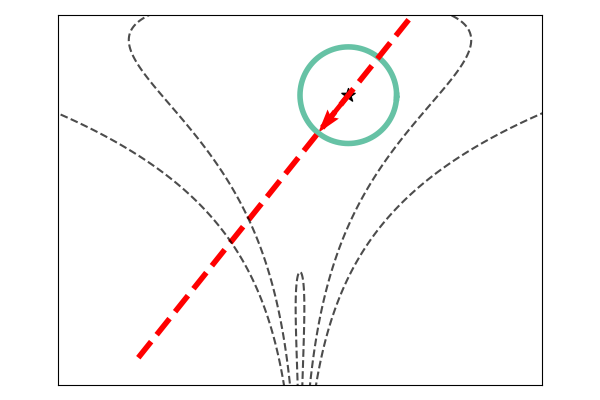
\includegraphics[width=0.49\linewidth]{figs/paper2/hitandrun/geodesic_balls_euclidean_hitandrun.png}
    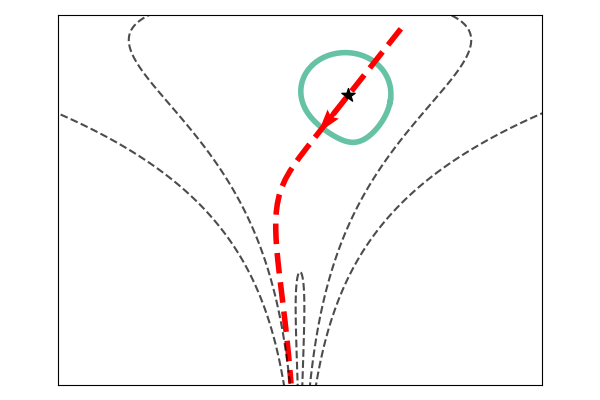
\includegraphics[width=0.49\linewidth]{figs/paper2/hitandrun/geodesic_balls_monge_hitandrun.png}
    \caption{Visualization of the hit-and-run procedure. Left:  A velocity uniformly sampled uniformly on $\mathbb{S}^{D-1}$ (blue) and the resulting straight line (dotted red line). Right:  A velocity sampled uniformly from $\{\boldsymbol{v}: \|\boldsymbol{v}\|^2_{\mathbf{G}(\boldsymbol{x})} =1\}$ and the geodesic captures better the geometry of the target (dotted red line).}
    \label{fig:hitandrun}
\end{figure}

\subsection{Geometric MCMC}
By geometric MCMC we refer to MCMC methods that incorporate a Riemannian tensor in the sampling method.
The main benefit is the adaptation to local curvature, but the introduction of a non-flat geometry results in higher computational cost. 
Recall that 
\begin{equation*}
 \mathbf{G}(\cdot):\mathbb{R}^D\to \mathbb{R}^D\times \mathbb{R}^D,   
\end{equation*}
is the matrix  that holds the components of a metric tensor (see Section~\ref{sec:riemannian_background}). 
Next we describe some geometric MCMC methods and their computational cost.

\paragraph{Riemannian manifold Hamiltonian Monte Carlo (RMHMC) }
The seminal work of \citet{Girolami2011} extended two gradient-based sampling methods,  Metropolis-adjusted Langevin algorithm (MALA) and Hamiltonian Monte Carlo (HMC) from Euclidean space to a Riemannian setting. Here we only describe the HMC extension. Both HMC and RMHMC introduce an auxiliary momentum $\boldsymbol{p}\in\mathbb{R}^D$ and model a system of ordinary differential equations (ODEs). The goal is that the solution to the ODEs generates samples that are further away from the initial state reducing sample correlation. The Hamiltonian equation is
\begin{equation*}
    \mathcal{H}(\boldsymbol{x},\boldsymbol{p})
    =
    \phi(\boldsymbol{x})
    +
    \frac{1}{2}\boldsymbol{p}^{\top}\mathbf{G}(\boldsymbol{x})^{-1}\boldsymbol{p},
\end{equation*}
where $\phi(\boldsymbol{x})=-\ell(\boldsymbol{x})+ \frac{1}{2}\log\det \mathbf{G}(\boldsymbol{x})$. The dynamics are given by the differential equations obtained from differentiation of $\mathcal{H}(\boldsymbol{x},\boldsymbol{p})$
\begin{equation}
    \dot{\boldsymbol{x}} = \mathbf{G}(\boldsymbol{x})^{-1}\boldsymbol{p},
    \quad
    \dot{\boldsymbol{p}} = - \nabla_{\boldsymbol{x}} \mathcal{H}(\boldsymbol{x},\boldsymbol{p}).
    \label{eq:rmhmc}
\end{equation}
The numerical integration of Equation~\ref{eq:rmhmc} relies on fixed point iteration \citep{Girolami2011}. Each step iterates until a specified tolerance is reached to generate a proposal, increasing the runtime. With a full rank metric tensor the resulting computations are of order $\mathcal{O}(D^3)$ at each iteration,  which limits its scalability to high dimensional problems.

\paragraph{Lagrangian dynamical Monte Carlo (LMC) }
\citet{Lan2015} expressed the Hamiltonian equations in terms of velocity instead of momentum through a change of variables  $\boldsymbol{v}=\mathbf{G}(\boldsymbol{x})^{-1}\boldsymbol{p}$, and the system dynamics become
\begin{equation}
    \dot{\boldsymbol{x}} = \boldsymbol{v},
    \quad
    \dot{\boldsymbol{v}} = -\boldsymbol{\eta}(\boldsymbol{x},\boldsymbol{v}) - \mathbf{G}(\boldsymbol{x})^{-1}\nabla_{\boldsymbol{x}}\phi(\boldsymbol{x}),
    \label{eqsLMC}
\end{equation}
where $[\boldsymbol{\eta}(\boldsymbol{x},\boldsymbol{v})]_k=\sum_{i,j}\Gamma^k_{ij}(\boldsymbol{x})\,v_i v_j$, and the Christoffel symbols $\Gamma_{ij}^k$ are defined in Equation~\ref{eq:christoffel_symbols}. 
The authors proposed a numerical integrator that is explicit and does not rely on fixed point iterations, improving the running time over RMHMC. Each step still computes inverses of the metric tensor and is $\mathcal{O}(D^3)$ in complexity which again limits its scalability to higher dimensions. One way of reducing the complexity of the numerical integrators is to use metrics with closed form inverses and determinants \citep{Hartmann2022}. Some metric choices are presented in Chapter~\ref{ch:mcmc}.
Additionally, the numerical integrator introduces two hyperparameters, the step-size and the number of steps, with several strategies available for selecting a value. \citet{williams2024geometric} discuss the choice of metric, numerical integrator, and hyperparameter adaptation in RMHMC and LMC. 

\section{Modeling discrete data} \label{sec:discrete_data}

We study two problems: discrete-data generation and classification. For generative modeling we consider flow matching and Riemannian flow matching, while for classification we use Gaussian processes. 
We first review flow-based models and a Riemannian flow matching approach used for generative modeling of discrete data, and then we review Gaussian process classification. Both approaches model a continuous latent process that produces discrete outputs via an $\arg\max$ operation. In the first case the latent model is flow based, and in the second it is a Gaussian process.  

\subsection{Discrete data generation}


We first discuss two continuous generative models that are building blocks: conditional flow matching which operates in the Euclidean space, then Riemannian flow matching which operates on manifolds. Then we present a method for discrete data generation which operates on the simplex and uses the Fisher geometry. 

\paragraph{Conditional flow matching (CFM)}
Conditional flow matching is a generative model for continuous data in the Euclidean space \citep{Albergo2023,Lipman2023,liu2023flow}. 
For $\boldsymbol{x}\in \mathbb{R}^D$, the model defines a vector field
$\boldsymbol{u}_t:\mathbb{R}^D\times[0,1]\to\mathbb{R}^D$,
which evolves data according to 
\begin{equation}
    \frac{d\boldsymbol{x}_t}{dt}=\boldsymbol{u}_t(\boldsymbol{x}_t), \qquad \boldsymbol{x}_t\sim p_t,
    \label{eq:cfm_ode}
\end{equation}
where the initial condition is a simple base distribution $p_0$ that allows direct generation of samples and density evaluation, and the final condition is the data distribution $p_1=p_{\mathrm{data}}$. The marginal probability path $\{p_t\}_{t\in[0,1]}$ is linked to $\boldsymbol{u}_t$ by the continuity equation, this gives the instantaneous change of variable formula, which is useful for computing log-densities
\begin{equation*}
    \dv[]{\log p_t(x_t)}{t} = - \div(u_t(x_t)).
\end{equation*}
In practice $\boldsymbol{u}_t$ is not available, instead a parametric model (usually a neural network) $\boldsymbol{v}_t^\theta$ is fit to the conditional vector fields $\boldsymbol{u}_t(\boldsymbol{x}_t\mid\boldsymbol{x}_0,\boldsymbol{x}_1)$, the resulting objective is
\begin{equation}
\mathcal{L}_{\mathrm{CFM}}(\theta)
= \mathbb{E}_{\substack{t\sim \mathrm{Unif}(0,1) \\ \boldsymbol{x}_0,\boldsymbol{x}_1\sim\pi(\boldsymbol{x}_0,\boldsymbol{x}_1)}}
  \left\| \boldsymbol{v}^\theta_t\big(\boldsymbol{x}_t\big) - \boldsymbol{u}_t(\boldsymbol{x}_t|\boldsymbol{x}_0,\boldsymbol{x}_1) \right\|_2^2, \label{eq:cfm_loss}
\end{equation}
 where $\pi$ is any coupling with marginals $p_0$ and $p_1$. \citet{Lipman2023} show that this conditional objective equals up to a constant, the objective for estimating $\boldsymbol{u}_t(\boldsymbol{x}_t)$ directly. Therefore, $\boldsymbol{v}^\theta_t\big(\boldsymbol{x}_t\big)$ is used in  Equation~\ref{eq:cfm_ode} to generate new data. The velocity field depends on the interpolation path between $\boldsymbol{x}_0$ and $\boldsymbol{x}_1$.  A common choice is the linear interpolation $\boldsymbol{x}_t=(1-t)\boldsymbol{x}_0+t\boldsymbol{x}_1$
which yields the constant conditional velocity
\[
\boldsymbol{u}_t(\boldsymbol{x}_t\mid\boldsymbol{x}_0,\boldsymbol{x}_1)=\dot{\boldsymbol{x}}_t=\boldsymbol{x}_1-\boldsymbol{x}_0.
\]
Two common options for the joint density of $\boldsymbol{x}_0,\boldsymbol{x}_1$ are the independent coupling $\pi(\boldsymbol{x}_0,\boldsymbol{x}_1)=p_0(\boldsymbol{x}_0)p_1(\boldsymbol{x}_1)$ and optimal-transport coupling.
The optimal transport coupling is approximated with mini-batch optimal transport and typically improves optimization stability while reducing the number of function evaluations needed at sampling time \citep{Tong2024}.


\paragraph{Riemannian conditional flow matching (RCFM)}
Conditional flow matching can be extended from Euclidean space to a Riemannian manifold $(\mathcal{M}, \mathbf{G})$ \citep{Chen2024}. 
Instead of a vector field in the Euclidean space $\mathbb{R}^D$, the vector field is defined on the tangent space of the manifold $\boldsymbol{u}_t(\boldsymbol{x})\in T_{\boldsymbol{x}}\mathcal{M}$. The resulting dynamics on the manifold are
\[
\frac{d\boldsymbol{x}_t}{dt} = \boldsymbol{u}_t(\boldsymbol{x}_t), \qquad \boldsymbol{x}_t\sim p_t,
\]
where the initial condition is a simple base distribution defined over $\mathcal{M}$.
The marginal probability paths are generated from $\boldsymbol{u}_t$ by the Riemannian version of the instantaneous change of variables 
\begin{equation*}
    \dv[]{\log p_t(\boldsymbol{x}_t)}{t} = - \operatorname{div}_{\mathbf{G}}(\boldsymbol{u}_t(\boldsymbol{x}_t)), 
\end{equation*}
where $\operatorname{div}_\mathbf{G}$ is the Riemannian divergence \citep{Lee2018}. Similarly to the Euclidean case, $\boldsymbol{u}_t$ is not available, but we can train the parametric model $\boldsymbol{v}_t^\theta$ using the conditional objective 
\begin{equation*}
\mathbb{E}_{\substack{t\sim \mathrm{Unif}(0,1) \\ \boldsymbol{x}_0,\boldsymbol{x}_1\sim\pi(\boldsymbol{x}_0,\boldsymbol{x}_1)} }
\left\|\boldsymbol{v}_t^\theta(\boldsymbol{x}_t){-}\boldsymbol{u}_t(\boldsymbol{x}_t\mid \boldsymbol{x}_0,\boldsymbol{x}_1)\right\|^2_{\mathbf{G}(\boldsymbol{x}_t)}.
\end{equation*}
Here $\| \boldsymbol{v}  \|_{\mathbf{G}(\boldsymbol{x}_t)} := \sqrt{\boldsymbol{v}^\top \mathbf{G}(\boldsymbol{x}_t)\boldsymbol{v} } $ is the norm induced by the metric $\mathbf{G}$ at $\boldsymbol{x}_t$. The tangent velocity field depends on the interpolation, a standard choice is the geodesic which connects $\boldsymbol{x}_0$ and  $\boldsymbol{x}_1$, defined by  $\boldsymbol{x}_t = \operatorname{Exp}_{\boldsymbol{x}_0}( t \boldsymbol{v})$ and $\boldsymbol{v} = \operatorname{Log}_{\boldsymbol{x}_0}(\boldsymbol{x}_1)$. This choice gives the conditional target velocity
\[
\boldsymbol{u}_t(\boldsymbol{x}_t\mid\boldsymbol{x}_0,\boldsymbol{x}_1)
=\frac{\operatorname{Log}_{\boldsymbol{x}_t}(\boldsymbol{x}_1)}{1-t}, \quad \boldsymbol{x}_t = \operatorname{Exp}_{\boldsymbol{x}_0}( t \operatorname{Log}_{\boldsymbol{x}_0}(\boldsymbol{x}_1)).
\]
When $\mathcal{M}=\mathbb{R}^D$ with the Euclidean metric, these expressions reduce to standard CFM.
If the manifold does not have closed form geodesics and logarithm map, then training and inference rely on approximations of these quantities. As in CFM, $\pi(\boldsymbol{x}_0,\boldsymbol{x}_1)$ can be the independent coupling or the optimal transport coupling. On the manifold, the geodesic distance of two points is the length of the geodesic between them, mini-batch optimal transport computes the transport cost with respect to this distance. 



\paragraph{Discrete data generation with the Fisher geometry}
\citet{Cheng2024} and \citet{Davis2024} introduced Categorical Flow Matching on Statistical Manifolds (SFM), a special case of Riemannian flow matching for discrete data. In this model the manifold is the simplex and the metric is the Fisher information metric. In practice, the flow could be modeled directly on the simplex, but computations become unstable near the boundaries, where discrete observations lie. SFM therefore models  Riemannian flow matching on the sphere instead. We first introduce the simplex geometry with the Fisher metric, then establish the isomorphism with the sphere, and finally specify the training and sampling procedures. 

Let $K$ be the number of categories and $D:=K-1$ the latent dimension. Consider the simplex $\Delta^{D}:=\{\boldsymbol{x}\in\mathbb{R}_{\ge 0}^{K}:\;\sum_{k=1}^{K}x_k=1\}$, and endow the space with the Fisher information metric of the categorical distribution \citep{Miyamoto2024}
\begin{equation*}
 \mathbf{G}_F(\boldsymbol{x}) = \mathrm{diag}\left(\frac{1}{\boldsymbol{x}_{1:D}}\right) + \frac{1}{x_K} \mathbf{1}\mathbf{1}^\top.
\end{equation*}
Under the Fisher metric, the space has the inner product for $\boldsymbol{u},\boldsymbol{v}\in T_{\boldsymbol{x}}\Delta^D$,
\begin{align*}
    \inp{\boldsymbol{u}}{\boldsymbol{v}}_{G_F(\boldsymbol{x})} = \sum_{i=1}^D \frac{u_iv_i}{x_i} + \frac{( \sum_{i=1}^D u_i)( \sum_{i=1}^D v_i)}{x_K}  = \sum_{i=1}^K \frac{u_i v_i}{x_i}.
\end{align*}
The last equality uses the tangent space constraint in the ambient space $T_{\boldsymbol{x}}\Delta^D = \{\boldsymbol{u}\in\mathbb{R}^K: \sum_{i=1}^K u_i = 0\}$ so $u_K = -\sum_{i=1}^D u_i $.
Note that the inner product is only defined on $\mathring{\Delta}^D$, since it is undefined on the boundary. The bijection between the simplex and the positive orthant of the sphere, together with its inverse, is given by
\begin{equation}
\begin{aligned}
\varphi: \Delta^{D} \to \mathbb{S}_+^{D}, \quad
&\boldsymbol{x}\mapsto \boldsymbol{z} = \sqrt{\boldsymbol{x}},\quad \text{and}\\
\varphi^{-1}: \mathbb{S}_+^{D} \to \Delta^{D}, \quad
&\boldsymbol{z} \mapsto \boldsymbol{x} = \boldsymbol{z}^2.
\end{aligned}
\label{eq:bij_sfm}
\end{equation}
$\mathbb{S}_{+}^{D} := \{ \boldsymbol{z} \in \mathbb{R}_{\ge 0}^{K} : \sum_{k=1}^{K} z_k^2 = 1 \}$, and the square root and squaring operations are applied component wise. 
This bijection (illustrated in Figure~\ref{fig:simplex-sphere-map}) is in fact an isomorphism between $(\Delta^D  , \mathbf{G}_F)$ and $(\mathbb{S}_{+}^{D}, \mathbf{G})$, where $\mathbf{G}$ is the canonical metric on the sphere \citep{Miyamoto2024}. The sphere is embedded in $\mathbb{R}^K$, and it inherits the ambient space inner product restricted to the tangent space, for $\boldsymbol{u},\boldsymbol{v}\in T_{\boldsymbol{z}} \mathbb{S}_{+}^{D}$,
\begin{equation*}
    \inp{\boldsymbol{u}}{\boldsymbol{v}}_G = \inp{\boldsymbol{u}}{\boldsymbol{v}}_2 = \sum_{i=1}^K u_i v_i.
\end{equation*} 
The geodesics in the sphere are the outer rings, the exponential and  logarithm map are
\begin{equation}
\begin{aligned}
\operatorname{Exp}_{\boldsymbol{z}}( t \boldsymbol{v}) 
&= \cos\!\bigl(t\|\boldsymbol{v}\|_2\bigr)\boldsymbol{z}
+ \sin\!\bigl(t\|\boldsymbol{v}\|_2\bigr)\frac{\boldsymbol{v}}{\|\boldsymbol{v}\|_2}, \text{ and}\\
\operatorname{Log}_{\boldsymbol{z}}(\boldsymbol{z}')
&= \frac{\theta}{\sin\theta}\Bigl(\boldsymbol{z}' - \cos(\theta)\boldsymbol{z}\Bigr), \text{ where }
\theta = \arccos\!\bigl(\inp{\boldsymbol{z}}{\boldsymbol{z}'}\bigr).
\end{aligned}
\label{eq:geo_sphere}
\end{equation}
\begin{figure}
  \centering
\begin{tikzpicture}
  \def\r{2}

  \begin{scope}
    \coordinate (O)  at (0,0);
    \coordinate (X1) at ({-\r/sqrt(10)}, {-\r/sqrt(10)});
    \coordinate (X2) at ({\r},0);
    \coordinate (X3) at (0,{\r});

    % Straight edges for the simplex
    \draw[line width=1.4pt] (X1) -- (X2);
    \draw[line width=1.4pt] (X1) -- (X3);
    \draw[line width=1.4pt] (X2) -- (X3);

    % Axes
    \draw[->] (O) -- ({-1.15*\r/sqrt(10)}, {-1.15*\r/sqrt(10)}) node[below] {$x_1$};
    \draw[->] (O) -- ({1.15*\r}, 0) node[right] {$x_2$};
    \draw[->] (O) -- (0, {1.15*\r}) node[above] {$x_3$};
    \node[anchor=north west] at (-1.5, 2.5) {\Large $\Delta^2$};

    \node[
      star,
      star points=5,
      star point ratio=2.25,
      fill=green!50!black,
      draw=green!50!black,
      minimum size=9pt,
      inner sep=0pt
    ] at (0.5,0.5) {};
    \node[above right, text=green!50!black] at (0.5,0.5) {$x$};
  \end{scope}

  \draw[<->, line width=2pt] (2.9,1.1) -- (5.3,1.1)
    node[midway, above, font=\Large] {$\varphi$}
    node[midway, below, font=\Large] {$\varphi^{-1}$};

  \begin{scope}[xshift=6.5cm]
    % Axes
    \draw[->] (0,0) -- ({-1.15*\r/sqrt(10)}, {-1.15*\r/sqrt(10)}) node[below] {$z_1$};
    \draw[->] (0,0) -- ({1.15*\r}, 0) node[right] {$z_2$};
    \draw[->] (0,0) -- (0, {1.15*\r}) node[above] {$z_3$};
    \node[anchor=north west] at (-1.5, 2.5) {\Large $\mathbb{S}_+^2$};

    % Arcs for the spherical section
    \draw[line width=1.4pt] (\r, 0) arc [start angle=0, end angle=90, x radius=\r, y radius=\r];
    \draw[line width=1.4pt] (0, \r) arc [start angle=90, end angle=198, x radius=\r/3, y radius=\r];
    \draw[line width=1.4pt] ({-\r/sqrt(10)}, {-\r/sqrt(10)}) arc [start angle=-108, end angle=0, x radius=\r, y radius=\r/3];
    
    \node[
      star,
      star points=5,
      star point ratio=2.25,
      fill=green!50!black,
      draw=green!50!black,
      minimum size=9pt,
      inner sep=0pt
    ] at (0.7,0.7) {};
    \node[above right, text=green!50!black] at (0.7,0.7) {$\varphi(x)$};
  \end{scope}
\end{tikzpicture}
  \caption{Visual illustration of the simplex-to-sphere map.}
  \label{fig:simplex-sphere-map}
\end{figure}


\begin{proposition}[Isometry, \citep{amari2000methods, Miyamoto2024}]
\label{prop:isomorphism_fisher}
The diffeomorphism in Equation~\ref{eq:bij_sfm} is an isomorphism between $(\Delta^D  , \mathbf{G}_F)$  and $(\mathbb{S}_{+}^{D}, \mathbf{G})$ up to a factor of $\frac{1}{4}$.
\end{proposition}
\begin{proof}
    The proof consists of showing
    $
    \frac{1}{4}\inp{\boldsymbol{u}}{\boldsymbol{v}}_{\mathbf{G}_F(\boldsymbol{x})}
    =
    \inp{\mathrm{d}\varphi_{\boldsymbol{x}}(\boldsymbol{u})}{\mathrm{d}\varphi_{\boldsymbol{x}}(\boldsymbol{v})}
    $
    for all $\boldsymbol{x}\in \Delta^D$ and $\boldsymbol{u},\boldsymbol{v}\in T_{\boldsymbol{x}}\Delta^D$, where $\mathrm{d}\varphi_{\boldsymbol{x}}(\boldsymbol{v})$ denotes the differential of $\varphi$ at $\boldsymbol{x}$ applied to the tangent vector $\boldsymbol{v}$. Since $\mathbb{S}_{+}^{D}$ is embedded in $\mathbb{R}^K$, we use the ambient Euclidean inner product
    \begin{align*}
        \inp{\mathrm{d}\varphi_{\boldsymbol{x}}(\boldsymbol{u})}{\mathrm{d}\varphi_{\boldsymbol{x}}(\boldsymbol{v})}
        &=
        \inp{\eval{\dv{}{t}\varphi(\boldsymbol{x}+t\boldsymbol{u})}_{t=0}}
            {\eval{\dv{}{t}\varphi(\boldsymbol{x}+t\boldsymbol{v})}_{t=0}} \\
        &=
        \inp{ \left(
\frac{u_1}{2\sqrt{x_1}},\dots,\frac{u_K}{2\sqrt{x_K}}
\right) }
            {\left(
\frac{v_1}{2\sqrt{x_1}},\dots,\frac{v_K}{2\sqrt{x_K}}
\right)} \\
        &= \frac{1}{4}\sum_{i=1}^K \frac{u_i v_i}{x_i}
        = \frac{1}{4}\inp{\boldsymbol{u}}{\boldsymbol{v}}_{\mathbf{G}_F(\boldsymbol{x})}.
    \end{align*}
\end{proof}
Based on the isomorphism (Proposition~\ref{prop:isomorphism_fisher}), the exponential map in $(\Delta^D  , \mathbf{G}_F)$ is 
\begin{align*}
\operatorname{Exp}_{\boldsymbol{x}}( t \boldsymbol{v})  &= \varphi^{-1}\big(\mathrm{Exp}_{\sqrt{x}}(d\varphi_x(v))\big) \\
& = \left(
\cos\!\left(\frac{t\|\boldsymbol{v}\|_{\mathbf{G}_F(\boldsymbol{x})}}{2}\right)\sqrt{\boldsymbol{x}}
+
\sin\!\left(\frac{t\|\boldsymbol{v}\|_{\mathbf{G}_F(\boldsymbol{x})}}{2}\right)
\frac{\boldsymbol{v}}{\|\boldsymbol{v}\|_{\mathbf{G}_F(\boldsymbol{x})}\sqrt{\boldsymbol{x}}}
\right)^2.
\label{eq:geo_simplex}
\end{align*}
Note that $\|\cdot \|_{\mathbf{G}_F}$ and $\tfrac{1}{\sqrt{\boldsymbol{x}}}$ explode when $\boldsymbol{x}$ approaches $\partial \Delta^D$ which makes it unstable, to address this  \citet{Cheng2024} and \cite{Davis2024} proposed modeling directly in the sphere. The approach first transforms the training data to the sphere with $\varphi$, and then fits the flow's parameters with RCFM on this space (Algorithm~\ref{alg:train_sfm}). New data is sampled by numerical integration of the learned velocity field, and the final point is mapped to the simplex with $\varphi^{-1}$ (Algorithm~\ref{alg:sample_sfm}).

\begin{algorithm}
\caption{Training of SFM.}
\label{alg:train_sfm}
\begin{algorithmic}[1]
\Require Data $\boldsymbol{x}\!\in\!\Delta^{D}$, bijection $\varphi$, base $p_0$ (e.g. $\varphi_\sharp \mathrm{Unif}(\Delta^D)$), 
coupling $\pi$ (indep. or minibatch OT)
\For{each mini-batch}    
  \State $\boldsymbol{z}_1 \gets \varphi({\boldsymbol{x}})$ \Comment{Map to the sphere.}
  \State Sample $\boldsymbol{z}_0 \sim p_0$; pair $(\boldsymbol{z}_0,\boldsymbol{z}_1)$ via $\pi$
  \State Sample $t\sim \mathrm{Unif}(0,1)$
  \State $\boldsymbol{z}_t\!\gets\!\operatorname{Exp}_{\boldsymbol{z}_0}( t \operatorname{Log}_{\boldsymbol{z}_0}(\boldsymbol{z}_1))$, \;
         $\boldsymbol{u}_t\!\gets\!{\operatorname{Log}_{\boldsymbol{z}_t}(\boldsymbol{z}_1)}/({1-t})$
  \State Update $\theta$ by 
  $\min \|\boldsymbol{v}_t^\theta(\boldsymbol{z}_t)-\boldsymbol{u}_t\|_{\mathbf{G}(\boldsymbol{z}_t)}^2$ \; 
\EndFor
\end{algorithmic}
\end{algorithm}

\begin{algorithm}[t]
\caption{Sampling with SFM.}
\label{alg:sample_sfm}
\begin{algorithmic}[1]
\Require Learned $\boldsymbol{v}_\theta$, bijection $\varphi$, base $p_0$
\State Sample $\boldsymbol{z}_0 \sim p_0$ 
\State Solve ODE: 
$\tfrac{d\boldsymbol{z}_t}{dt} = \boldsymbol{v}_\theta(\boldsymbol{z}_t,t), \; t\!\in[0,1], \boldsymbol{z}_t\in \mathbb{S}^D$
\State $\hat{\boldsymbol{x}} \gets \varphi^{-1}(\boldsymbol{z}_1)$
\end{algorithmic}
\end{algorithm}

\subsection{Gaussian processes for classification} \label{sec:gp}

We first briefly introduce Gaussian processes.  We then describe two sparse formulations based on inducing points. Finally we present Dirichlet-based Gaussian process classification, which uses label smoothing and a distributional approximation to turn classification into Gaussian process regression in the latent space. These topics provide together the background for Paper~IV.

\paragraph{Gaussian process}

A Gaussian process (GP) \citep{williams2006gaussian} defines a distribution over functions such that any finite collection of function values is jointly Gaussian. It provides a flexible prior together with uncertainty quantification. Given a finite set of inputs $\boldsymbol{x}_1,\ldots,\boldsymbol{x}_N\in\mathbb{R}^P$ the distribution over values $(f(\boldsymbol{x}_1), .., f(\boldsymbol{x}_N))$ is multivariate Gaussian, where the mean is specified by a mean function $m:\mathbb{R}^P\to\mathbb{R}$ and the covariance between any pair of points by a kernel $K_\theta:\mathbb{R}^P\times\mathbb{R}^P\to\mathbb{R}$ dependent on hyperparameters $\theta$. The GP prior is written  as 
\[
f \sim \mathcal{GP}\!\bigl(m(\cdot),\,K_{\theta}(\cdot,\cdot)\bigr).
\]
Consider a supervised regression problem where the data is denoted $\mathcal{D}:=\{(\boldsymbol{x}_n,\boldsymbol{z}_n)\}_{n=1}^N$ for $\boldsymbol{x}_n\in\mathbb{R}^P$ and $\boldsymbol{z}_n\in\mathbb{R}^D$. 
In practice, the responses are usually centered by subtracting the empirical mean, and the mean function is set to zero. 
The kernel function imposes assumptions on the correlation of the latent functions and on the behavior of the function space. For example, different kernels can model periodic behaviors, or be translation invariant. In this work we consider the radial basis function kernel
\[
K_{\theta}(\boldsymbol{x},\boldsymbol{x}')
=
\sigma_f^2\exp\!\left(-\frac{\|\boldsymbol{x}-\boldsymbol{x}'\|_2^2}{2\ell^2}\right),
\qquad
\theta=(\sigma_f^2,\ell),
\]
where $\sigma_f^2$ controls the variance and $\ell$ is the length scale which controls how fast the dependency between $\boldsymbol{x}$ and $\boldsymbol{x}'$ decays. This kernel gives smooth latent functions. 

Although it is possible to introduce dependency among dimensions \citep{goulard1992linear}, in this thesis, we model $D$ independent GPs (one per dimension) denoted $\mathbf{f} = (f^{(1)}, .., f^{(D)})$, and the same kernel is shared across $D$-dimensions. 
Given a  GP prior assume the noisy Gaussian likelihood
 \[
\boldsymbol z_n\mid \mathbf f(\boldsymbol{x}_n) \sim \mathcal N\!\bigl(\mathbf f(\boldsymbol{x}_n),\,\sigma^2\mathbf I_D\bigr).
\]
Let $\boldsymbol{x}_*\in\mathbb{R}^P$ be a test input and denote the vector of responses $\boldsymbol{z}^{(d)} := \bigl(z_1^{(d)},\ldots,z_N^{(d)}\bigr)^\top \in \mathbb{R}^N$ for $d=1,..,D$. The joint distribution of $\boldsymbol{z}^{(d)}$ and $f^{(d)}(\boldsymbol{x}_*)$ is
\begin{equation*}
\begin{bmatrix}
\boldsymbol{z}^{(d)} \\
f^{(d)}(\boldsymbol{x}_*)
\end{bmatrix}
\sim
\mathcal{N}\!\left(
\boldsymbol{0},
\begin{bmatrix}
\mathbf{K}_N + \sigma^2 \mathbf{I}_N & \mathbf{k}_* \\
\mathbf{k}_*^\top & k_{**}
\end{bmatrix}
\right),
\end{equation*}
where the covariance entries are given by
$[\mathbf{K}_N]_{ij} = k_\theta(\boldsymbol{x}_i,\boldsymbol{x}_j)$, $[\mathbf{k}_*]_i = k_\theta(\boldsymbol{x}_i,\boldsymbol{x}_*)$, and $k_{**} = k_\theta(\boldsymbol{x}_*,\boldsymbol{x}_*)$.
The standard predictive posterior is obtained by conditioning on the observations  \citep{williams2006gaussian}, it is distributed as
$f^{(d)}(\boldsymbol{x}_*) \mid \boldsymbol{z}^{(d)}
\sim
\mathcal{N}\!\bigl(\mu_*^{(d)},\,\sigma_*^2\bigr)$ with mean and covariance
\begin{equation}
\begin{aligned}
\mu_*^{(d)} &:=\mathbf k_*^\top(\mathbf{K}_{N}+\sigma^2\mathbf I_N)^{-1}\boldsymbol z^{(d)}, \text{ and}\\
\sigma_*^2 &:= k_{**}-\mathbf k_*^\top(\mathbf{K}_{N}+\sigma^2\mathbf I_N)^{-1}\mathbf k_*.
\end{aligned}
\label{eq:gp_posterior}
\end{equation}
We can write it compactly in a single expression
\begin{equation*}
 \mathbf f_*\mid\mathcal D\sim\mathcal N(\boldsymbol\mu_*,\boldsymbol\Sigma_*),   
\end{equation*}
with $\boldsymbol\mu_*:=(\mu_*^{(1)},\ldots,\mu_*^{(D)})^\top$ and $\boldsymbol\Sigma_*:=\sigma_*^2\mathbf I_D$. The marginal log-likelihood is used to learn the kernel hyperparameters. Since the likelihood is Gaussian and the output dimensions are assumed independent, it takes the form 
\begin{equation}
\log p\bigl(\boldsymbol{z} \mid \theta\bigr)
= -\tfrac12\sum_{d=1}^D \|\boldsymbol z^{(d)}\|^2_{(\mathbf{K}_{N}+\sigma^2\mathbf I_N)^{-1}}
- \tfrac{D}{2}\log\lvert\mathbf{K}_{N}+\sigma^2\mathbf I_N\rvert, 
\label{eq:mll}
\end{equation}
where the constant terms that do not depend on $\theta$ are dropped.

\paragraph{Sparse Gaussian process}

Exact GP inference scales cubically in complexity with the number of training points, which prohibits its use with data points in the thousands. Sparse GP methods reduce this cost by using a smaller set $M\ll N$ of inducing points  $\mathbf{X}_{\mathrm u}:=\{\boldsymbol{x}^{\mathrm u}_m\}_{m=1}^M$.
Denote the inducing variables for each dimension by
\begin{equation*}
    \mathbf{u}^{(d)} := f^{(d)}(\mathbf{X}_{\mathrm u}) \in \mathbb{R}^M.
\end{equation*}
We first introduce the \emph{uncollapsed} variational formulation \citep{Hensman2013}, and then the \emph{collapsed} formulation \citep{titsias2009variational}. 
These methods use a variational Gaussian distribution 
\begin{equation*}
    q(\mathbf u)=\prod_{d=1}^D q(\mathbf u^{(d)}),
\qquad
q(\mathbf u^{(d)})=\mathcal N\!\bigl(\mathbf u^{(d)} \mid \mathbf m^{(d)}, \mathbf S^{(d)}\bigr),
\end{equation*}
and define the approximation to the process
\begin{equation*}
    q(\mathbf f^{(d)}) = \int p(\mathbf f^{(d)} \mid \mathbf u^{(d)})\,q(\mathbf u^{(d)})\,d\mathbf u^{(d)}.
\end{equation*}
Similar to the derivation of Equation~\ref{eq:elbo}, the approximate process results in the following lower bound 
\begin{equation}
\log p(\boldsymbol{z})
\geq
\sum_{d=1}^D \mathbb E_{q(\mathbf f^{(d)})}\!\left[\log p\bigl(\boldsymbol{z}^{(d)}\mid \mathbf f^{(d)}\bigr)\right]
-\sum_{d=1}^D \mathrm{KL}\bigl[q(\mathbf u^{(d)})\,\|\,p(\mathbf u^{(d)})\bigr].
\label{eq:lower_bound_uncollapsed}
\end{equation}
For the Gaussian approximation, the expected log likelihood factorizes over the data points
\begin{equation*}
 \log p(\boldsymbol z) \geq\sum_{d=1}^D \sum_{n=1}^N \mathbb{E}_{q(f^{(d)}_n)}\!\left[ \log 
 \mathcal{N}(z^{(d)}_n\mid f^{(d)}_n, \sigma^2)\right]
-\sum_{d=1}^D \mathrm{KL}\bigl[q(\mathbf u^{(d)})\,\|\,p(\mathbf u^{(d)})\bigr].   
\end{equation*}
This is the \emph{uncollapsed} bound. Since the first term is additive over the data it is possible to use stochastic optimization giving a complexity of $\mathcal{O}(BM^2 + M^3)$ for a batch size $B$. The variational parameters $\{\mathbf m^{(d)},\mathbf S^{(d)}\}_{d=1}^D$ and the inducing points are optimized together.

The \emph{collapsed} bound is obtained by observing that the variational parameters $\{\mathbf m^{(d)},\mathbf S^{(d)}\}_{d=1}^D$ can be optimized analytically \citep{titsias2009variational}. This leads to a bound that only depends on the inducing point locations and is not additive over the input data
\begin{equation}
\log p(\mathbf z)
\;\ge\;
\sum_{d=1}^D
\log \mathcal N\!\left(
\mathbf z^{(d)} \mid \mathbf 0,\,
\mathbf Q_{N}
+ \sigma^2 \mathbf I_N
\right)
\;-\;
\frac{D}{2\sigma^2}
\operatorname{tr}\!\left(
\mathbf K_{N} - \mathbf Q_{N}
\right),
\label{eq:lower_bound_collapsed}
\end{equation}
where $\mathbf Q_{N} = \mathbf K_{NM}\mathbf K_{M}^{-1}\mathbf K_{MN}$ is the low rank covariance matrix given by the inducing points, and $\mathbf K_{NM}$ denotes the covariance between training and inducing inputs. The first term is the log-likelihood of a Gaussian process with $\mathbf{Q}_N$ replacing $\mathbf{K}_N$, while the second term penalizes the discrepancy between $\mathbf K_{N}$ and $\mathbf Q_{N}$. The complexity of the collapsed method is $\mathcal{O}(NM^2)$. If the inducing points are the training points then $\mathbf{K}_N = \mathbf{Q}_N$ and the objective is exact and coincides with the marginal log-likelihood. 

The predictions over a new data point $\boldsymbol{x}_*$ are obtained by the predictive distribution given by the inducing variables
\begin{equation*}
    q\bigl(f_*^{(d)}\bigr)=\int p\bigl(f_*^{(d)}\mid \mathbf u^{(d)}\bigr)\,q(\mathbf u^{(d)})\,d\mathbf u^{(d)},
\end{equation*}
which has a closed form because $q(\mathbf u^{(d)})$ is Gaussian. In the \emph{uncollapsed} case the parameters of the variational Gaussian are optimized with respect to Equation~\ref{eq:lower_bound_uncollapsed}. In the \emph{collapsed} case the parameters are given analytically as solutions from Equation~\ref{eq:lower_bound_collapsed}. The complexity of the predictions is cubic on $M$.

\paragraph{Dirichlet-based Gaussian process classification}
Gaussian process classification estimates class probabilities from latent Gaussian processes. Let us consider classification with $K$ categories where the data is $\mathcal D=\{(\boldsymbol{x}_n,c_n)\}_{n=1}^N$ for class $c_n\in\{1,\dots,K\}$ and covariate $\boldsymbol{x}_n\in \mathbb{R}^P$. The class probabilities are denoted $\boldsymbol\pi(\boldsymbol{x})\in \Delta^D$. A standard GP classifier introduces $K$ latent Gaussian processes, giving the model 
\begin{equation*}
    f_k(\cdot)\sim \mathcal{GP}\!\bigl(0,\,K_{\theta}(\cdot,\cdot)\bigr),\quad 
    c|\boldsymbol{x}\sim \mathrm{Cat}\left(\mathrm{softmax}\!\bigl(\mathbf f(\boldsymbol{x})\bigr) \right),
\end{equation*}
where $\mathbf f(\boldsymbol{x})= (f^{(1)}(\boldsymbol{x}), .., f^{(K)}(\boldsymbol{x}))^\top$. The categorical likelihood is not conjugate with the Gaussian prior and posterior inference relies on approximations, such as variational inference \citep{Hensman2015}.

Dirichlet-based Gaussian process classification (GPD) \citep{milios2018dirichlet} avoids this non-conjugacy by converting classification to a regression problem in a latent space. Instead of modeling the class probabilities directly with a link function (e.g. softmax), it places a Dirichlet distribution on the probabilities
\begin{equation*}
    \boldsymbol\pi(\boldsymbol{x})\mid \boldsymbol{x} \sim \mathrm{Dir}\!\bigl(\boldsymbol\alpha(\boldsymbol{x})\bigr).
\end{equation*}
The Dirichlet parameters are modeled with GPs. 
Conditional on a label $c=k$, the parameters of the Dirichlet distribution are chosen as 
\[
\alpha_k = \mathbf{1}\{c=k\} + \alpha_{\varepsilon}, \qquad k=1,\ldots,K,
\]
where $\alpha_\varepsilon\geq 0$ is a smoothing parameter such that  as $\alpha_\varepsilon\to 0$ the Dirichlet distribution concentrates on the one-hot vector $\mathbf{e}_k$. The distribution is generated by $K$-independent Gamma random variables distributed $g_j\stackrel{\text{ind}}{\sim}\mathrm{Gamma}(\alpha_j,1)$ and $\boldsymbol{\pi}$ is recovered by normalization
\begin{equation*}
 \pi_k = \frac{g_k}{\sum_{\ell=1}^K g_{\ell}}\iff \boldsymbol{\pi} = \operatorname{softmax}(\log \boldsymbol{g}).
\end{equation*}
To make the model conjugate, GPD approximates each Gamma distribution with a log-normal random variable $\mathrm{Lognormal}(\tilde{y}_j,\tilde{\sigma}_j^2)$, matching the first two moments
\begin{equation}
\begin{aligned}
\tilde{\sigma}_k^2&=\log\!\left(1+\tfrac{1}{\alpha_k}\right),
\qquad
\tilde{y}_k=\log \alpha_k-\tfrac{1}{2}\tilde{\sigma}_k^2.
\end{aligned}
\label{eq:lognorm}
\end{equation}
Under the log-normal approximation the model is conjugate in log space. The method fits $K$-independent GPs to the transformed data  $\tilde{y}_{nj}$ with heteroscedastic noise variance $\tilde{\sigma}_{nj}^2$, where both $\tilde{y}_{nj}$ and $\tilde{\sigma}_{nj}^2$ depend on the class label and the smoothing parameter.
At a test input $\boldsymbol{x}_*$, inference for the latent variable $\mathbf f_*$ is exact, but class probabilities are computed after the softmax map and are estimated with Monte Carlo
\[
\begin{aligned}
\mathbb E[\boldsymbol\pi_* \mid \boldsymbol{x}_*,\mathcal D]
&\approx \frac{1}{S}\sum_{s=1}^S \mathrm{softmax}\bigl(\mathbf f_*^{(s)}\bigr),\\
\mathbf f_*^{(s)} &\sim p(\mathbf f_* \mid \boldsymbol{x}_*,\mathcal D).
\end{aligned}
\]
Note that since GP classification is converted to GP regression on the smoothed labels $\tilde{y}$, it can directly use  sparse Gaussian processes or any other scalable regression machinery.

\chapter{Advances in Geometric Bayesian Inference} \label{ch:mcmc}
In this chapter we propose using the geometry of the log target density in two different inference methods for drawing samples. The first one (Paper I) is a distributional approximation to the target distribution using a generalization of the Laplace approximation. The second one (Paper II) uses MCMC and generalizes the hit-and-run slice-sampler to a particular Riemannian setting in which geodesics are not closed form. 

This chapter starts by introducing common elements between our contributions. These elements rely on the notions of Riemannian geometry presented in Chapter~\ref{ch:background}.
We introduce choices for the metric tensor, the volume, the Hausdorff density, and discuss the numerical computation of the exponential map. Then, we present the Riemannian Laplace approximation with the Fisher metric and the geodesic slice sampler for multimodal distributions with strong curvature. 

\paragraph{Motivation}
Equipping the space with a non Euclidean geometry increases computational complexity (dependent on the metric choice), but can lead to higher quality samples. In particular, it enables exploration of curved regions of the parameter space and better captures multimodal distributions compared to Euclidean methods.

\section{Choice of metric tensor} \label{sec:geometric_tools}

We consider a target density $p(\boldsymbol{x})$ defined over $\mathbb{R}^D$ with respect to the Lebesgue measure. We give the Euclidean space the Riemannian metric $\mathbf{G}(\boldsymbol{x})$. Once the metric is fixed it determines the local geometry of the space and determines the geometric objects used in this chapter such as geodesics, logarithm map and volume elements.

\subsection{Riemannian metrics}
The Riemannian metrics we consider in this chapter depend on the probabilistic model, through the log density $\log p(\boldsymbol{x})$, and each of them leads to a different geometry. Next we introduce the metric choices,  and give the corresponding inverse, determinant and Christoffel symbols needed for geodesic computations.


\paragraph{Euclidean metric}
Let us present Euclidean space using the same tools as more general cases. Euclidean space is equipped with a constant metric, 
\begin{equation*}
 \mathbf{G}(\boldsymbol{x}) = \mathbf{I}_D.
\end{equation*}
The Christoffel symbols vanish $\Gamma_{ij}^k=0$ for all $i,j,k=1,\ldots,D$ and the exponential and logarithm map are, for $\boldsymbol{x},\boldsymbol{y} \in \mathbb{R}^D$ and $\boldsymbol{v} \in T_{\boldsymbol{x}} \mathbb{R}^D \cong \mathbb{R}^D$,
\begin{equation}\label{eq:Euclidean_exp_log}
\begin{aligned}
\operatorname{Exp}_{\boldsymbol{x}}(t\boldsymbol{v}) &= \boldsymbol{x} + t\boldsymbol{v}, \text{ and}\\
\operatorname{Log}_{\boldsymbol{x}}(\boldsymbol{y}) &= \boldsymbol{y} - \boldsymbol{x}.
\end{aligned}
\end{equation}
The volume measure is the usual Lebesgue measure, geodesics are straight lines and all operations are available in closed form. The inverse metric $\mathbf{G}^{-1}$ is again the identity, and the determinant is one. In other words, we obtain the usual properties of the Euclidean metric.

\paragraph{Fisher metric}
Let us consider a probabilistic model such that target density is $p_{\mathcal{Y}|\mathcal{X}}(\boldsymbol{y}\mid\boldsymbol{x})\,p_{\mathcal{X}}(\boldsymbol{x})$.
The Fisher information matrix \citep{fisher1925theory, amari2000methods} is defined as 
\begin{equation}
 \mathbf{G}(\boldsymbol{x}) = \mathbb{E}_{\mathcal{Y}|\mathcal{X}}\left[ \nabla_{\boldsymbol{x}} \log p_{\mathcal{Y}|\mathcal{X}}(\boldsymbol{y}\mid\boldsymbol{x})
 \nabla_{\boldsymbol{x}} \log p_{\mathcal{Y}|\mathcal{X}}(\boldsymbol{y}\mid\boldsymbol{x}) ^\top
 \right]. \label{eq:fisher_information_metric}
\end{equation}
The Fisher information can be motivated by the local approximation to the Kullback-Leibler divergence between two nearby distributions. Consider the models at $\boldsymbol{x}$ and $\boldsymbol{x}+d\boldsymbol{x}$, a second order Taylor expansion gives
\begin{equation*}
\begin{aligned}
\log p_{\mathcal{Y}|\mathcal{X}}(\boldsymbol{y}\mid\boldsymbol{x} + d\boldsymbol{x})
&\approx \log p_{\mathcal{Y}|\mathcal{X}}(\boldsymbol{y}\mid\boldsymbol{x})
+ \inp{ d\boldsymbol{x} }{ \nabla_{\boldsymbol{x}} \log p_{\mathcal{Y}|\mathcal{X}}(\boldsymbol{y}\mid\boldsymbol{x}) } \\
&\quad + \tfrac{1}{2} \|d\boldsymbol{x}\|_{ \nabla^2_{\boldsymbol{x}} \log p_{\mathcal{Y}|\mathcal{X}}(\boldsymbol{y}\mid\boldsymbol{x}) }
+ \mathcal{O}(\| d\boldsymbol{x} \|^3).
\end{aligned}
\end{equation*}
Plugging in the Taylor expansion and using the identities $\int \pi(x) \nabla \log \pi(x) =0$ and 
$\mathbf{G}(\boldsymbol{x}) = \mathbb{E}_{\mathcal{Y}|\mathcal{X}}\left[ -\nabla^2_{\boldsymbol{x}} \log p_{\mathcal{Y}|\mathcal{X}}(\boldsymbol{y}\mid\boldsymbol{x}) \right]$, we get
\begin{equation*}
    \operatorname{KL}(p_{\mathcal{Y}|\mathcal{X}}(\boldsymbol{y}\mid\boldsymbol{x}) \,\|\, p_{\mathcal{Y}|\mathcal{X}}(\boldsymbol{y}\mid\boldsymbol{x} + d\boldsymbol{x}) ) = \frac{1}{2} d\boldsymbol{x}^\top \mathbf{G}(\boldsymbol{x}) d\boldsymbol{x} + \mathcal{O}(\| d\boldsymbol{x}  \| ^3).
\end{equation*}
Hence, the Fisher metric captures the local geometry of the likelihood under the KL-divergence.
A remarkable property of the Fisher information is given by \v{C}encov's theorem \citep{vcencov1982statistical}. It states that the Fisher information metric is the unique Riemannian metric up to a rescaling constant that is invariant under sufficient statistical mappings. 

Some downsides of the Fisher metric are computational. It depends on the probabilistic model and the expectation with respect to $\mathcal{Y}\mid\mathcal{X}$ might be intractable for some models, for example, if the likelihood is a Gaussian mixture. Another difficulty is that the metric is usually full-rank, meaning computation of the inverse $\mathbf{G}^{-1}(\boldsymbol{x})$ and the determinant have cubic complexity on $D$. If the exponential map computation requires numerical integration, then each integration step has cubic complexity because the Christoffel symbols (Equation~\ref{eq:christoffel_symbols}) use the metric's inverse.

The Fisher information metric (Equation~\ref{eq:fisher_information_metric}) is defined in terms of the likelihood. However, in Bayesian inference one is interested in the posterior distribution, which depends on both $p_{\mathcal{Y}|\mathcal{X}}(\boldsymbol{y}\mid\boldsymbol{x})$ and the prior $p_{\mathcal{X}}(\boldsymbol{x})$. In this case, the Fisher information incorporates both terms, by adding the Hessian of the log-prior \citep{Girolami2011},
\begin{equation}
 \mathbf{G}(\boldsymbol{x}) = \mathbb{E}_{\mathcal{Y}|\mathcal{X}}\left[ \nabla_{\boldsymbol{x}} \log p_{\mathcal{Y}|\mathcal{X}}(\boldsymbol{y}\mid\boldsymbol{x})
 \nabla_{\boldsymbol{x}} \log p_{\mathcal{Y}|\mathcal{X}}(\boldsymbol{y}\mid\boldsymbol{x}) ^\top
 \right]  + \nabla^2 \log p_{\mathcal{X}}(\boldsymbol{x}).
 \label{eq:fisher_w_prior}
\end{equation}


\paragraph{Monge metric}
Recall $\ell(\boldsymbol{x}) = \log p(\boldsymbol{x})$ and consider the graph of the tempered log-density
\begin{equation*}
\mathcal{G}_{\alpha}
:=
\left\{
(\boldsymbol{x}, \alpha \ell(\boldsymbol{x}))
\,:\,
\boldsymbol{x}\in \mathbb{R}^D
\right\}
\subset \mathbb{R}^{D+1},
\qquad \alpha \geq 0.    
\end{equation*}
This is a $D$ dimensional manifold embedded in $\mathbb{R}^{D+1}$ (see Section~\ref{sec:riemannian_background}). The Monge metric is the Riemannian tensor on $\mathbb{R}^{D+1}$ given by this embedding \citep{Hartmann2022},
\begin{equation*}
    \mathbf{G}(\boldsymbol{x}) = \mathbf{I}_D + \alpha^2 \nabla \ell(\boldsymbol{x})\nabla \ell(\boldsymbol{x})^\top.
\end{equation*}
This metric is more efficient than the Fisher metric because the inverse, determinant and Christoffel symbols are computable and depend on first and second order derivatives of the log-density which are computed efficiently with automatic differentiation (hessian vector products) and enables the metric to be used in higher dimensional problems such as Bayesian neural networks \citep{Bergamin2024, yu2023scalable}.

The inverse metric and square-root metric are obtained by the Sherman-Morrison lemma
\begin{align*}
    \mathbf{G}^{-1}(\boldsymbol{x}) &= \mathbf{I}_D 
    - \frac{\alpha^2}{1+\alpha^2 \|\nabla \ell(\boldsymbol{x})\|^2} \nabla \ell(\boldsymbol{x}) \nabla \ell(\boldsymbol{x})^\top, \text{ and}\\
    \mathbf{G}^{1/2}(\boldsymbol{x})&= \mathbf{I}_D + \frac{\alpha^2}{\sqrt{1 + \alpha^2\|\nabla\ell(\boldsymbol{x})\|^2} + 1} \nabla\ell(\boldsymbol{x})\nabla\ell(\boldsymbol{x})^\top.
\end{align*}
The determinant is $\det \mathbf{G}(\boldsymbol{x}) = 1 + \alpha^2\|\nabla \ell(\boldsymbol{x})\|^2$ and the Christoffel symbols stacked into $D$ matrices, of shape $D\times D$ are
\begin{equation}
    \Gamma^{k}(\boldsymbol{x}) = \frac{\alpha^2 \partial_k \ell(\boldsymbol{x})}{1+\alpha^2\norm{\nabla\ell(\boldsymbol{x})}^2}\nabla^2\ell(\boldsymbol{x}). 
    \label{eq:christoffel_symbols_monge}
\end{equation}
The Monge metric has the property that it \emph{slows down} geodesics that start from a local mode: the Euclidean distance covered by a geodesic is strictly smaller than the distance covered by a straight line. Observation~\ref{obs:monge} formally states this phenomenon. This contraction is the factor causing the bias in Riemannian Laplace approximation under the Monge metric (see Section~\ref{sec:rla}).

\begin{observation} \label{obs:monge}
Let $\boldsymbol{x}_0$ be the MAP estimate. Let $\boldsymbol{v}_0 \neq \boldsymbol{0}$ and let 
$\boldsymbol{x}_1 = \operatorname{Exp}_{\boldsymbol{x}_0}(\boldsymbol{v}_0)$ denote the exponential
map at time $t=1$ under the Monge metric. Then
\begin{equation*}
    \|\boldsymbol{x}_1 - \boldsymbol{x}_0\|_2 < \|\boldsymbol{v}_0\|_2.
\end{equation*}
\end{observation}

\begin{proof}
Since $\nabla\ell(\boldsymbol{x}_0) = \boldsymbol{0}$, the Monge metric at $\boldsymbol{x}_0$ reduces 
to the identity, and the initial speed satisfies $\|\boldsymbol{v}_0\|_{\mathbf{G}(\boldsymbol{x})}^2 = \|\boldsymbol{v}_0\|_2^2$.
Along any geodesic the metric speed is conserved, so
\begin{equation*}
    \|\boldsymbol{v}_0\|^2_2=\|\dot{\boldsymbol{x}}(t)\|^2_{\mathbf{G}(\boldsymbol{x}(t))}  = \|\dot{\boldsymbol{x}}(t)\|_2^2 + \alpha^2
    \inp{\nabla\ell(\boldsymbol{x}(t))}{\dot{\boldsymbol{x}}(t)}^2    
    , \qquad \forall\, t\in[0,1].
\end{equation*}
and rearranging gives
\begin{equation*}
    \|\dot{\boldsymbol{x}}(t)\|_2^2 
    = \|\boldsymbol{v}_0\|_2^2 - \alpha^2\!\left(\frac{d}{dt}\ell(\boldsymbol{x}(t))\right)^{\!2} 
    \leq \|\boldsymbol{v}_0\|_2^2,
\end{equation*}
with equality only when $\frac{d}{dt}\ell(\boldsymbol{x}(t)) = 0$.
Differentiating $\frac{d}{dt}\ell(\boldsymbol{x}(t))$ w.r.t $t$
and evaluating at $t=0$, and using $\nabla\ell(\boldsymbol{x}_0)=\boldsymbol{0}$ one obtains
\begin{equation*}
    \frac{d}{dt}\Bigl[\nabla\ell(\boldsymbol{x}(t))^\top\dot{\boldsymbol{x}}(t)\Bigr]\bigg|_{t=0}
    = \boldsymbol{v}_0^\top\nabla^2\ell(\boldsymbol{x}_0)\,\boldsymbol{v}_0.
\end{equation*}
Since $\nabla^2\ell(\boldsymbol{x}_0)\prec 0$ and $\boldsymbol{v}_0\neq\boldsymbol{0}$, this 
derivative is strictly negative. By continuity, there exists $\epsilon > 0$ such that
\begin{equation*}
    \frac{d}{dt}\ell(\boldsymbol{x}(t)) \neq 0 
    \quad\Longrightarrow\quad 
    \|\dot{\boldsymbol{x}}(t)\|_2 < \|\boldsymbol{v}_0\|_2, 
    \qquad \forall\, t\in(0,\epsilon).
\end{equation*}
By the triangle inequality
\begin{equation*}
    \|\boldsymbol{x}_1 - \boldsymbol{x}_0\|_2 
    = \left\|\int_0^1 \dot{\boldsymbol{x}}(t)\,dt\right\|_2 
    \leq \int_0^1\|\dot{\boldsymbol{x}}(t)\|_2\,dt 
    < \int_0^1\|\boldsymbol{v}_0\|_2\,dt 
    = \|\boldsymbol{v}_0\|_2,
\end{equation*}
where the strict inequality holds because $\|\dot{\boldsymbol{x}}(t)\|_2 \leq \|\boldsymbol{v}_0\|_2$ 
everywhere with strict inequality on $(0, \epsilon)$, a set of positive measure.
\end{proof}


\paragraph{Generative metric}
The generative metric \citep{Kim2024} rescales the Euclidean geometry according to the inverse target density. This metric makes motion through high density regions cheaper than motion through low density regions. 
As a result, geodesic curves tend to  ``prefer'' areas where the target density is large, see Observation~\ref{obs:generative}. Figure~\ref{fig:metric_visualization} illustrates the Monge and generative metrics capturing the geometry of a curved distribution. Define the generative metric
\begin{figure} 
    \centering
    \begin{subfigure}[b]{0.4\linewidth}
        \centering
        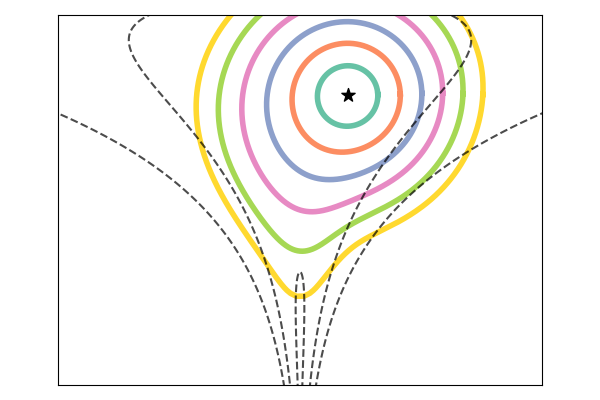
\includegraphics[width=\linewidth]{figs/paper2/geodesic_balls_generative.png}
        \caption{Generative metric.}
    \end{subfigure}
    \begin{subfigure}[b]{0.4\linewidth}
        \centering
        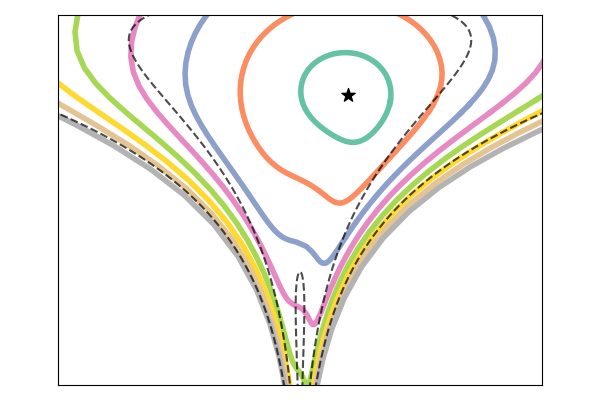
\includegraphics[width=\linewidth]{figs/paper2/geodesic_balls_monge.png}
        \caption{Monge metric.}
    \end{subfigure}
    \begin{subfigure}[b]{0.4\linewidth}
        \centering
        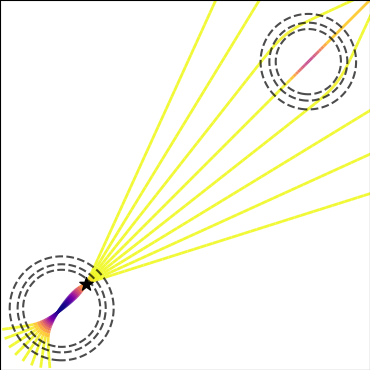
\includegraphics[width=0.8\linewidth]{figs/paper2/geodesic_inverse_generative.png}
        \caption{Inverse generative metric.}
    \end{subfigure}    
    \begin{subfigure}[b]{0.4\linewidth}
        \centering
        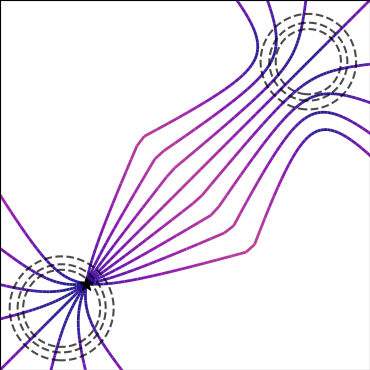
\includegraphics[width=0.8\linewidth]{figs/paper2/geodesic_inverse_monge.png}
        \caption{Inverse Monge metric.}
    \end{subfigure}    
    \caption{Visualization of the generative, inverse generative, Monge and inverse Monge metrics. \textbf{Top:} geodesic balls of varying radii centered at $\star$. \textbf{Bottom:} geodesics originating at $\star$ with different initial velocities (yellow indicates higher speed). The Monge metric deviates more from the Euclidean geometry than the generative metric, while the generative metric accelerates more in low-density regions.
   }
    \label{fig:metric_visualization}
\end{figure}
\begin{equation*}
    \mathbf{G}(\boldsymbol{x}) = \rho(\boldsymbol{x})^2 \mathbf{I}_D,
    \qquad
    \rho(\boldsymbol{x}) := \frac{p_0 + \lambda}{p(\boldsymbol{x}) + \lambda},
\end{equation*}
where $p_0, \lambda>0$ prevent the metric from becoming singular when $p(\boldsymbol{x})$ is small.
Since this metric is the identity matrix scaled, the inverse and determinant are straight to compute. The Christoffel symbols depend only on the gradient of the scalar factor,
\begin{equation*}
\Gamma^k(\boldsymbol{x}) = \nabla \log \rho(\boldsymbol{x}) \,\boldsymbol{e}_k^\top
+ \boldsymbol{e}_k \,\nabla \log \rho(\boldsymbol{x})^\top
- \partial_k \log \rho(\boldsymbol{x}) \,\mathbf{I}_D.
\end{equation*}

\begin{observation}[High-density regions are cheaper under the generative metric] \label{obs:generative}
Let
\begin{equation*}
\mathbf G(\boldsymbol x)=\rho(\boldsymbol x)^2 \mathbf I_D,
\qquad
\rho(\boldsymbol x)=\frac{p_0+\lambda}{p(\boldsymbol x)+\lambda},
\qquad p_0,\lambda>0.    
\end{equation*}
Then the Riemannian length of a piecewise \(C^1\) curve \(\gamma:[0,1]\to\mathbb R^D\) is
\begin{equation*}
L_{\mathbf G}(\gamma)=
\int_0^1
\|\dot \gamma(t)\|_{\mathbf G(\gamma(t))} \,
d t
=
\int_0^1 \left(\frac{p_0+\lambda}{p(\boldsymbol x)+\lambda}\right) \|\dot\gamma(t)\|_2\,dt.    
\end{equation*}
This weighted average results in geodesics that have a tradeoff between higher density values and shorter velocity Euclidean norms.
\end{observation}


\paragraph{The inverse metrics}
We have now introduced the Fisher, Monge and generative metrics. Now, we propose using the inverse metric to sample multimodal distributions. In general, any Riemannian tensor that is positive definite and full rank is mathematically valid. In particular, the inverse of the metrics is also positive definite and defines a valid metric tensor. This motivates defining the inverse metric
\begin{equation}
\boxed{
    \mathbf{G}_{\mathrm{inv}}(\boldsymbol{x}) = \mathbf{G}^{-1}(\boldsymbol{x}).
}
\end{equation}
The determinant is $\det \mathbf{G}_{\mathrm{inv}}(\boldsymbol{x})  = 1/\det \mathbf{G}(\boldsymbol{x})$. The Christoffel symbols are analytic and computable with automatic differentiation for the Monge and generative metrics. 

By Observations~\ref{obs:monge} and~\ref{obs:generative} the Monge and generative metrics induce geodesics that tend to stay within regions of high density. By using the inverse metric we hope to ``revert'' this property. In regions of low density, both the generative and Monge metrics assign larger Euclidean metric values, so their inverses effectively ``speed up'' motion.
As a result, geodesics can cover larger Euclidean distances over the same amount of geodesic time. This behavior is formalized in Observations~{\ref{obs:invmonge}} and~{\ref{obs:invgen}}. Figure~\ref{fig:metric_visualization} illustrates the properties of the inverse generative and inverse Monge metrics on a bimodal distribution. Although this does not guarantee that a geodesic will move from one mode to another in dimensions $D\geq 2$, we empirically observe in Section~\ref{sec:geodesic_slice} that the geodesics under the inverse Monge metric are capable of traversing between modes of multimodal distributions. 

\begin{observation}[Paper II]
\emph{
    Let $p(\boldsymbol{x})$ be a smooth density function. Let $(\boldsymbol{x}_t, \boldsymbol{v}_t)$ be the geodesic flow with initial conditions $(\boldsymbol{x}_0,\boldsymbol{v}_0)$  with respect to the inverse Monge metric, such that $\boldsymbol{x}_0$ is a local maximum.
    Then $\norm{\boldsymbol{v}_t}_{2}\geq \norm{\boldsymbol{v}_0}_{2}$ 
    for all $t\neq 0$.
    } \label{obs:invmonge}
\end{observation}
\begin{observation}[Paper II]
\emph{
    Let $p(\boldsymbol{x})$ be a smooth density function. Let $(\boldsymbol{x}_t, \boldsymbol{v}_t)$ be the geodesic flow with initial conditions $(\boldsymbol{x}_0,\boldsymbol{v}_0)$ such that $p(\boldsymbol{x}_0)>0$ with respect to the inverse generative metric. Then, for $t$ such that $p(\boldsymbol{x}_t) \to 0$ we have $\norm{\boldsymbol{v}_t}_{2}>\norm{\boldsymbol{v}_0}_{2}$.
    } \label{obs:invgen}
\end{observation}


 
\subsection{Volume form and density on the manifold}

\paragraph{Geodesic balls}
In both methods considered later,  we need to sample tangent vectors at a unit geodesic distance of a fixed point. 
For $\boldsymbol{x}\in\mathbb{R}^D$ the tangent space sphere of radius $r$ is
\begin{equation*}
\mathbb{S}^{D-1}_{\mathbf{G},r}(\boldsymbol{x})
:=
\left\{
\boldsymbol{v}\in T_{\boldsymbol{x}}\mathbb{R}^D :
\|\boldsymbol{v}\|_{\mathbf{G}(\boldsymbol{x})}= r
\right\}.
\end{equation*}
In practice we need to sample uniformly from the tangent space unit sphere which can be done as follows:
\begin{enumerate}
    \item Sample $\boldsymbol{v} \sim \mathcal{N}(\boldsymbol{0}, \mathbf{G}^{-1}(\boldsymbol{x}))$.
    \item Normalize $\boldsymbol{v} \leftarrow {\boldsymbol{v}}/{\|\boldsymbol{v}\|_{\mathbf{G}(\boldsymbol{x})}}$.
\end{enumerate}
Note that sampling $\boldsymbol{v} \sim \mathcal{N}(\boldsymbol{0}, \mathbf{G}^{-1}(\boldsymbol{x}))$ requires computing the inverse square root matrix $\mathbf{G}^{-1/2}$ which requires generally Cholesky decomposition, but for the Monge, generative, inverse Monge and inverse generative metrics it admits an analytic form. 

\paragraph{Hausdorff density}
The original target density $p(\boldsymbol{x})$ is defined with respect to Lebesgue measure in $\mathbb{R}^D$. Once a Riemannian metric is introduced, the natural reference measure becomes the Riemannian volume element \citep{Lee2018}, which is
\begin{equation*}
    d\mathrm{vol}_{\mathbf{G}}(\boldsymbol{x}) = \sqrt{\det \mathbf{G}(\boldsymbol{x})}\,d\boldsymbol{x}.
\end{equation*}
If we want to represent the density with respect to the volume element instead of Lebesgue measure, it must be rescaled by the corresponding factor.  We refer to this density as the Hausdorff density and write
\begin{equation} 
  p_{\mathcal{H}}(\boldsymbol{x}) := \frac{p(\boldsymbol{x})}{\sqrt{\det \mathbf{G}(\boldsymbol{x})}}. \label{eq:hausdensity}
\end{equation}
This is consistent with change of variables formula. Consider the  diffeomorphism  $\boldsymbol{z} = \varphi(\boldsymbol{x})$, change of variables gives
\begin{equation*}
    p_{\mathcal{Z}}(\boldsymbol{z}) = p(\varphi^{-1}(\boldsymbol{z})) \left|\det \mathbf{J}_{\varphi^{-1}}(\boldsymbol{x})\right|.
\end{equation*}
If $\mathbf{G}$ is the push-forward of the Euclidean metric under $\varphi$, then $\mathbf{G}(\boldsymbol{z})  = \mathbf{J}_{\varphi^{-1}}(\boldsymbol{z})^\top
    \mathbf{J}_{\varphi^{-1}}(\boldsymbol{z})$, and hence $\sqrt{\det \mathbf{G}(\boldsymbol{z})} = \left|\det \mathbf{J}_{\varphi^{-1}}(\boldsymbol{z})\right|$, and the change of variables formula can be written as
\begin{equation*}
    p_{\mathcal{Z}}(\boldsymbol{z}) = p(\varphi^{-1}(\boldsymbol{z}))  \sqrt{\det \mathbf{G}(\boldsymbol{z})}.
\end{equation*}
The density with respect to the Riemannian volume measure is
\begin{equation*}
    p_{\mathcal H}(\boldsymbol{z})
    =
    \frac{p_{\mathcal{Z}}(\boldsymbol{z})}{\sqrt{\det \mathbf{G}(\boldsymbol{z})}}. 
\end{equation*}
That is, the Hausdorff density removes the Jacobian volume factor and gets the density expressed with respect to the geometry induced by the metric.



\subsection{Numerical computation of geodesics}
For the Euclidean metric we can easily compute the exponential and logarithmic maps as in Equation~\ref{eq:Euclidean_exp_log}, but for the other metric choices we solve the geodesic equations numerically. Let $\boldsymbol{x}(t)$ denote the geodesic trajectory and $\boldsymbol{v}(t)=\boldsymbol{\dot x}(t)$ its velocity. Equation~\ref{eq:geodesic_equations} is rewritten as
\begin{align}
      \boldsymbol{ \dot x}(t)  &= \boldsymbol{v}(t), \nonumber \\
    \dot v_k(t) &= - \boldsymbol{v}(t)^\top\Gamma^k(\boldsymbol{x}(t))  \boldsymbol{v}(t), \quad  k = 1, \ldots, D, \label{eq:geoeqs}
\end{align}
where $\Gamma^k(\boldsymbol{x})\in\mathbb{R}^{D\times D}$ is the matrix with the Christoffel symbols (Equation~\ref{eq:christoffel_symbols}). 
The main computational bottleneck comes from the Christoffel symbols, since they involve the inverse metric and derivatives of the metric. The Fisher metric in general has $\mathcal{O}(D^3)$ complexity, the Monge and inverse Monge metrics have the complexity of Hessian-vector products, and the generative and inverse generative metrics have the complexity of gradient computations.

The choice of numerical solver affects accuracy and runtime \citep{kidger2022neural}. Fixed step-size, adaptive and higher order solvers introduce tradeoffs between stability, numerical error and computational cost. We conduct empirical studies on the choice of numerical solver for different metric choices in Section~\ref{sec:geodesic_slice}.



\begin{table}[t]
\centering
\footnotesize
\setlength{\tabcolsep}{4pt}
\begin{adjustbox}{max width=\linewidth}
\begin{tabular}{@{}lccc@{}}
\toprule
 & \textbf{Funnel} & \textbf{Rosenbrock} & \textbf{Squiggle} \\
\midrule
$\varphi(\boldsymbol{z})$
&
$\left[
\begin{array}{c}
e^{\sigma z_D /2} \boldsymbol{z}_{1:D-1}\\
\sigma z_D
\end{array}
\right]$
&
$\left[
\begin{array}{c}
a + \tfrac{1}{\sqrt{2}}z_1 \\
\left(a + \tfrac{1}{\sqrt{2}}z_1\right)^2 + \tfrac{1}{\sqrt{2b}}z_2
\end{array}
\right]$
&
$\left[
\begin{array}{c}
z_1 \\
\boldsymbol{z}_{2:D} - \sin(a z_1)
\end{array}
\right]$
\\
\midrule
$p(\boldsymbol{x})$
&
$\begin{aligned}
&\mathcal{N}(x_D \mid 0,\sigma^2)\\
&\times\mathcal{N}(\boldsymbol{x}_{1:D-1} \mid \boldsymbol{0}, e^{x_D}\mathbf{I}_{D-1})
\end{aligned}$
&
$\begin{aligned}
&\mathcal{N}(x_1 \mid a, \tfrac{1}{2})\\
&\times\mathcal{N}(x_2 \mid x_1^2, \tfrac{1}{2b})
\end{aligned}$
&
$\begin{aligned}
&\mathcal{N}\!\bigl(\varphi^{-1}(\boldsymbol{x}) \mid \boldsymbol{\mu}, \mathbf{\Sigma}\bigr)\\
&\times\left|\det \mathbf{J}_{\varphi^{-1}}(\boldsymbol{x})\right|
\end{aligned}$
\\
\midrule
&
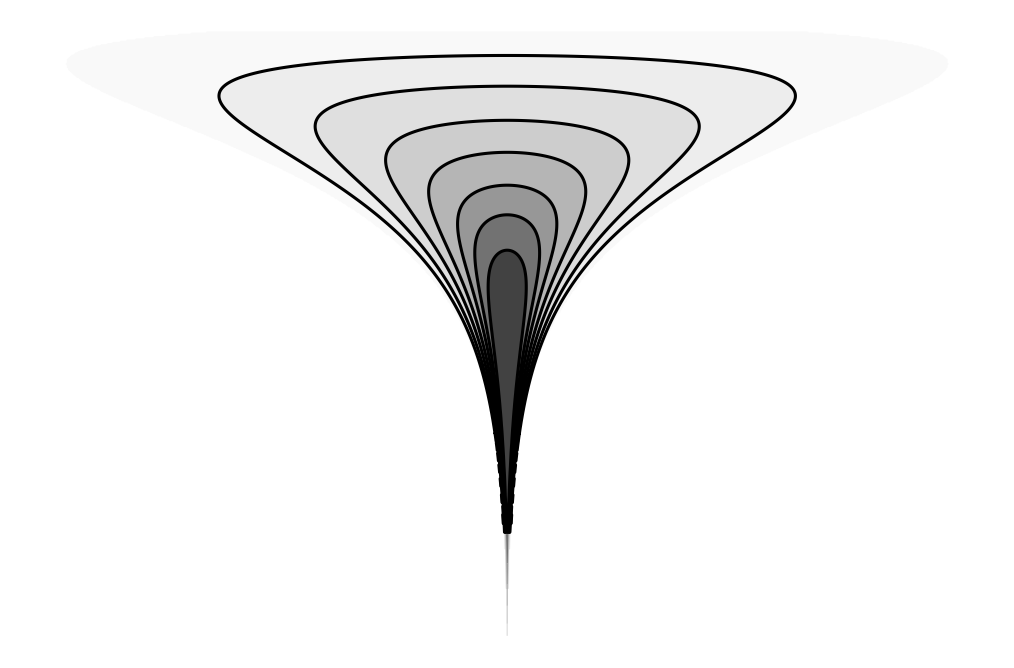
\includegraphics[width=0.32\linewidth]{figs/extra/funnel_contour.png}
&
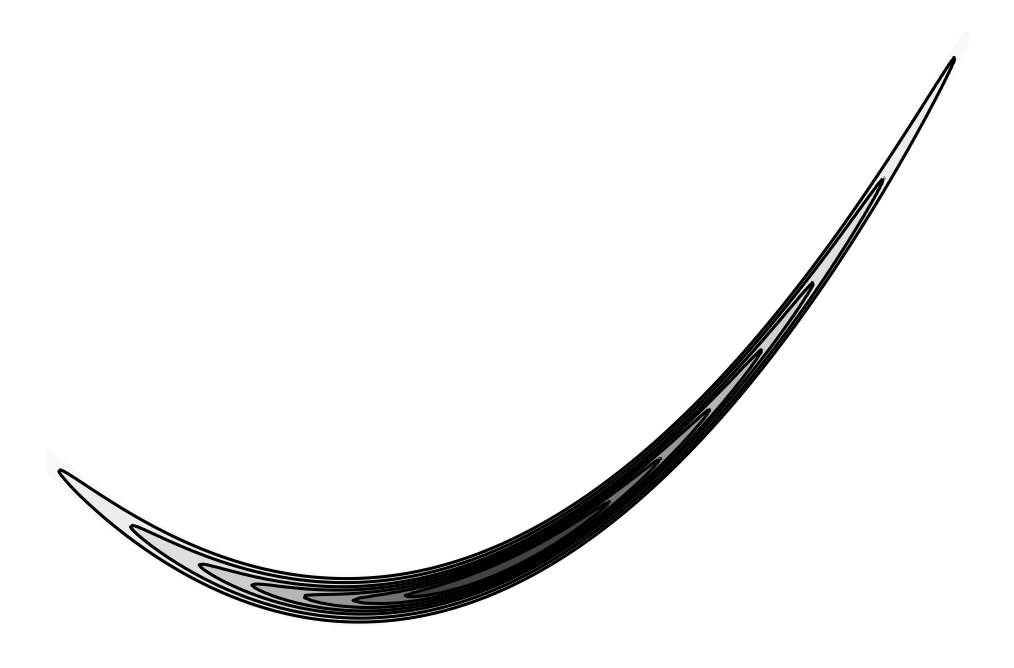
\includegraphics[width=0.32\linewidth]{figs/extra/rosenbrock_contour.png}
&
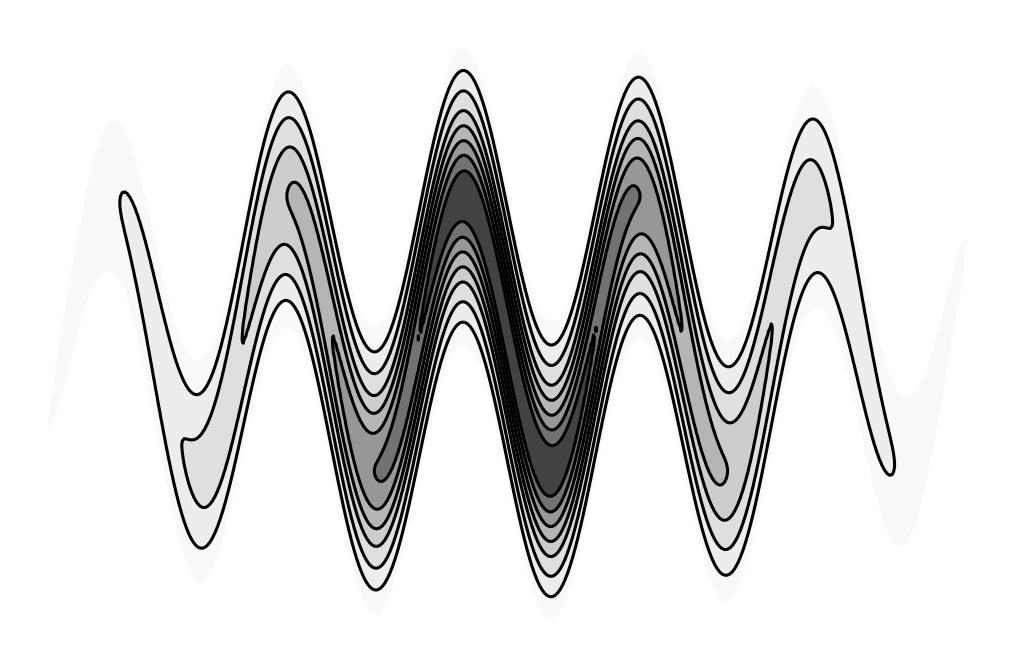
\includegraphics[width=0.32\linewidth]{figs/extra/squiggle_contour.png} \\
% \bottomrule 
\end{tabular}
\end{adjustbox}
\caption{Three benchmark distributions with strong curvature used in the experiments.}
\label{tab:curved_distributions}
\end{table}

\subsection{Target distributions with strong curvature} \label{sec:curved}
The need for a non-Euclidean metric is most pronounced in regions of the parameter space that are narrow along certain directions but still carry significant probability mass. For evaluation of these methods we hence consider three distributions with strong curvature that are constructed from a diffeomorphism of a standard Gaussian. They are the Funnel, Hybrid Rosenbrock and Squiggle distributions. Here we present a simpler version of the Hybrid Rosenbrock, the $D$-dimensional version is given in \citet{Pagani2022}. Table~\ref{tab:curved_distributions} shows the distributions, summarizes the transformations and the corresponding target densities.

The latent value is distributed  $\boldsymbol{z}\sim \mathcal{N}(\boldsymbol{\mu},\mathbf{\Sigma})$ and $\boldsymbol{x}=\varphi(\boldsymbol{z})$.
The bijection $\varphi$ allows the generation of samples for benchmarking. The pullback metric follows from the transformation rule of Riemannian tensors,
\begin{equation}
\mathbf{G}(\boldsymbol{x})
=
\mathbf{J}_{\varphi^{-1}}(\boldsymbol{x})^\top
\mathbf{\Sigma}^{-1}
\mathbf{J}_{\varphi^{-1}}(\boldsymbol{x}).
\label{eq:pullback_metric_curved}
\end{equation}

\section{Case study I: Riemannian Laplace approximation} \label{sec:rla}

We apply the geometric tools we have described above in the construction of Riemannian Laplace approximation (RLA) \citep{Bergamin2024}. We first use a second order Taylor approximation to motivate placing a Gaussian distribution in the tangent space at the mode. Sampling is then done by drawing Gaussian velocities in this tangent space, and pushing them forward with the exponential map. RLA can be viewed as an exponential wrapped Gaussian approximation where the geometry is determined by the chosen metric tensor (see Figure~\ref{fig:rla}).
\begin{figure}
    \centering
    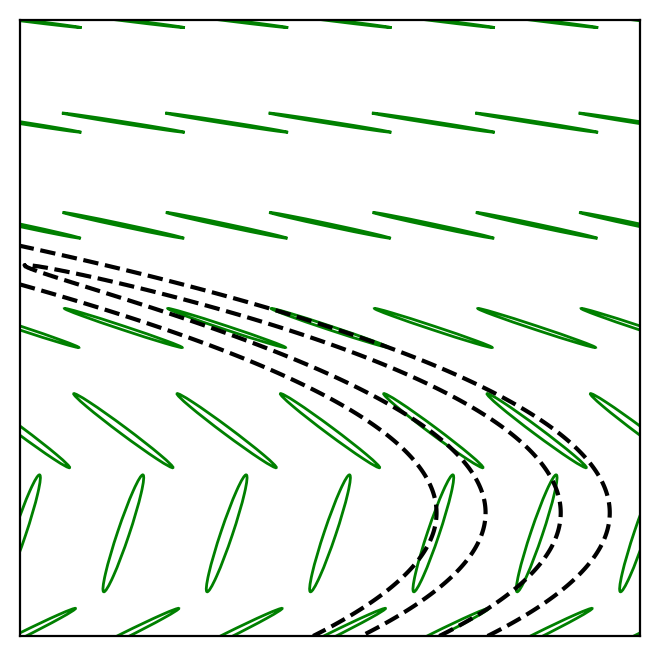
\includegraphics[width=0.3\linewidth]{figs/paper1/metrics.png}
    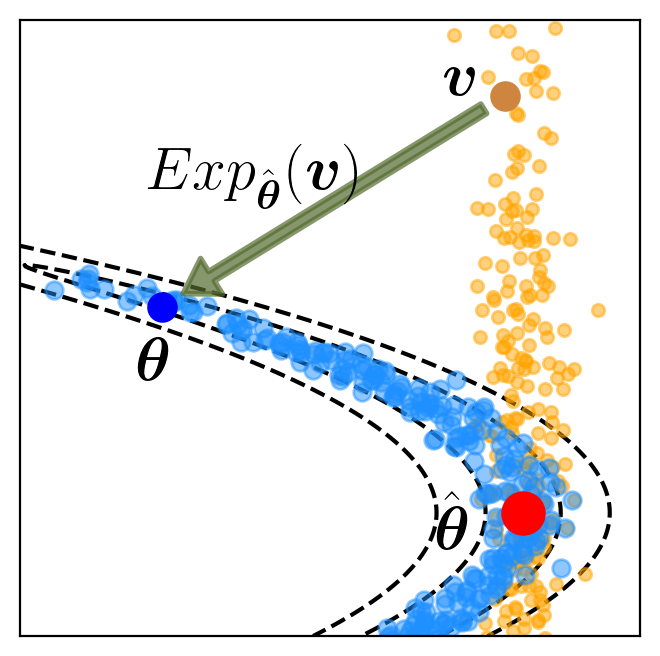
\includegraphics[width=0.3\linewidth]{figs/paper1/geodesics.png}
    \caption{Visualization of Riemannian Laplace approximation. The Fisher metric (green) captures the local curvature. Right: Samples from a Gaussian distribution (orange) are deterministically mapped using the Fisher metric to provide a flexible approximation (blue).}
    \label{fig:rla}
\end{figure}

Let $f$ be a scalar output function defined on the manifold and $c(t)$ a curve on the manifold such that $c(0)= \boldsymbol{x}$. As given in Section~5.9, Equation~5.26, of \citet{Boumal2023}, the second-order Taylor approximation is
\begin{equation} \label{eq:taylor_mfd}
    \begin{aligned}
    f(c(t)) = f(\boldsymbol{x})
&+ t \left\langle \nabla_{\mathbf{G}} f(\boldsymbol{x}), \boldsymbol{v} \right\rangle_{\mathbf{G}(\boldsymbol{x})}
+ \frac{t^2}{2} \left\langle \operatorname{Hess}_{\mathbf{G}} f(\boldsymbol{x})[\boldsymbol{v}], \boldsymbol{v} \right\rangle_{\mathbf{G}(\boldsymbol{x})} \\
&+ \frac{t^2}{2} \left\langle \nabla_{\mathbf{G}} f(\boldsymbol{x}), \ddot{c}(0) \right\rangle_{\mathbf{G}(\boldsymbol{x})}
+ \mathcal{O}(t^3).        
    \end{aligned}
\end{equation}
Let $\ell$ be the target logdensity (Euclidean or Hausdorff) and $\hat{\boldsymbol{x}}$ a local maximum of $\ell$. 
At the mode $\hat{\boldsymbol{x}}$, both Euclidean and Riemannian gradients vanish, and a second order Taylor expansion of $\ell$ along geodesics (Equation~\ref{eq:taylor_mfd})  simplifies to
\begin{equation}\label{eq:riemlap}
\ell\big(\operatorname{Exp}_{\hat{\boldsymbol{x}}}(\boldsymbol{v})\big)
\approx \ell(\hat{\boldsymbol{x}})
+ \tfrac{1}{2}\, 
\left\langle
\operatorname{Hess}_{\mathbf{G}}\,\ell(\hat{\boldsymbol{x}})[\boldsymbol{v}],
\boldsymbol{v}
\right\rangle_{\mathbf{G}(\boldsymbol{\hat{x}})},
\end{equation}
where $t$ is absorbed into $\boldsymbol{v}\gets t \boldsymbol{v}$. 
Furthermore, the Riemannian Hessian components (Equation~\ref{eq:riem_hessian}) simplify to
\begin{equation*}
 \mathrm{Hess}_{\mathbf{G}} \ell(\boldsymbol{\hat{x}}) [\boldsymbol{v}] = \mathbf{G}^{-1}(\boldsymbol{\hat{x}})\nabla^2\ell ({\boldsymbol{\hat{x}}}) \boldsymbol{v},
\end{equation*}
since $\nabla \ell(\hat{\boldsymbol{x}}) = \boldsymbol{0}$ \footnote{personal communication with Marcelo Hartmann}.
Thus, the quadratic term in Equation~\ref{eq:riemlap} is 
$\boldsymbol{v}^{\top}\nabla^2\ell(\hat{\boldsymbol{x}})\boldsymbol{v}$
, which motivates a tangent space Gaussian density
\begin{equation*}
 h_{\mathbf{\Sigma}}(\boldsymbol{v})=\mathcal{N}(\boldsymbol{v}\mid\boldsymbol{0}, \mathbf\Sigma), \quad   \mathbf\Sigma = \left(-\nabla^2\ell(\hat{\boldsymbol{x}})\right)^{-1}. 
\end{equation*} 
Samples that approximate the target are generated by mapping the exponential map on the tangent velocities (see Algorithm~\ref{alg:rla}), this is the core principle of the method
\begin{equation}
\boxed{
    \boldsymbol{x}=\operatorname{Exp}_{\hat{\boldsymbol{x}}}(\boldsymbol{v}), \quad \boldsymbol{v}\sim \mathcal{N}(\boldsymbol{0}, \mathbf\Sigma).
    }
\end{equation}
We can compute the RLA logdensity associated to the samples in the tangent space radius where the exponential map is injective  \citep{chevallier2022exponential}.
The push-forward density of the tangent Gaussian
with respect to the Riemannian volume is given by the exponential-wrapped change of variables
\begin{equation*}
\log q_{\mathcal H}(\boldsymbol{x})
=
\log h_{\mathbf{\Sigma}}(\boldsymbol{v})
-
\log \left|\det J_{\hat{\boldsymbol{x}}}(\boldsymbol{v}) \right|,
\end{equation*}
where $\boldsymbol{x}=\operatorname{Exp}_{\hat{\boldsymbol{x}}}(\boldsymbol{v})$ and  $\mathbf{J}_{\hat{\boldsymbol{x}}}(\boldsymbol{v})= \mathrm{d}_{\boldsymbol{v}}
\operatorname{Exp}_{\hat{\boldsymbol{x}}}(\boldsymbol{v})$. In general RLA settings the differential of the exponential map may need to be computed numerically. On affine locally symmetric spaces, however, it admits an explicit curvature-based series expansion, which yields tractable Jacobian formulas \citep{chevallier2022exponential}.
 

\begin{algorithm}[t]
	    \caption{RLA, producing $N$ samples $\boldsymbol{x}^{(n)}$.}    
	    \begin{algorithmic}[1]        
	    \Require Metric $\mathbf{G}$ and covariance $\mathbf{\Sigma}$
	        \State Obtain the MAP estimate $\hat{\boldsymbol{x}}$.        
	        \For{$n \leftarrow 1\dots N$}            
	            \State Obtain $\boldsymbol{v}^{(n)}\sim \mathcal{N}(\boldsymbol{0}, \mathbf{\Sigma})$
	            \State Push-forward $\boldsymbol{x}^{(n)} \gets \operatorname{Exp}_{\hat{\boldsymbol{x}}}(\boldsymbol{v}^{(n)})$
	        \EndFor
	\end{algorithmic}
	\label{alg:rla}
\end{algorithm}

\citet{Bergamin2024} proposed using the Monge metric in the RLA approximation, which we denote RLA-B. Although the Monge metric has lower complexity than Fisher metric, this approximation is biased for Gaussian targets as a consequence of  Observation~\ref{obs:monge}. The Monge geodesics contract Euclidean distances near a mode and samples generated by the geodesics under this metric are too close to the mode, while the Euclidean Laplace is exact. 

Paper I proposes two improvements that correct this behavior:
\begin{itemize}
    \item Apply a logarithm map to correct the magnitude of the velocities. Namely, replace Step~3 in Algorithm~\ref{alg:rla} with 
    \begin{align*}
	\tilde{\boldsymbol{x}}^{(n)} &\sim \mathcal{N}\!\left(\hat{\boldsymbol{x}}, (-\nabla^2 \ell(\hat{\boldsymbol{x}}))^{-1}\right), \text{ and} \\
	\boldsymbol{v}^{(n)} &= \operatorname{Log}_{\mathcal{P},\hat{\boldsymbol{x}}}(\tilde{\boldsymbol{x}}^{(n)}),
	\end{align*}    
    where $\operatorname{Log}_{\mathcal{P},\hat{\boldsymbol{x}}}$ is computed with respect to the Monge metric induced by the density $\mathcal{N}\!\left(\hat{\boldsymbol{x}}, (-\nabla^2 \ell(\hat{\boldsymbol{x}}))^{-1}\right)$, we refer to this variant as RLA-BLog.
    \item Use the Fisher information metric in Riemannian Laplace approximation, denoted RLA-F.
\end{itemize}

Additionally, Paper~I studies practical choices: whether the approximation should be centered at the Euclidean MAP or at the Hausdorff MAP and whether $\mathbf{\Sigma}=(-\nabla^2\ell(\boldsymbol{\hat{x}}))^{-1}$ or $\mathbf{\Sigma}=\mathbf{G}^{-1}(\boldsymbol{\hat{x}})$ should be used.
Paper~I also provides theoretical advantages for the Fisher metric. It is exact for Gaussian targets, asymptotically for targets that are Gaussian in the limit of infinite data, and it is  exact for targets that are diffeomorphic to a Gaussian. Theorem~\ref{thm:invariant-exact} states the exactness of RLA-F for Gaussian diffeomorphism. 

\begin{theorem}[\textbf{Paper I - Theorem 3}]
    With an invariant prior, e.g. Jeffreys prior, 
    RLA-F with Hausdorff MAP is exact for probabilistic models whose target distributions are diffeomorphic with Gaussians, for which the negative Hessian at the Hausdorff MAP coincides with the Fisher metric.
\label{thm:invariant-exact}
\end{theorem}


\subsection*{Empirical evaluation}
The empirical study compares Euclidean Laplace approximation (ELA), the Monge-based approximation (RLA-B), the logarithm-map corrected Monge variant (RLA-BLog), and the Fisher variant (RLA-F).
Here we include two of the experiments from Paper~I, the objective of the first experiment is to visually illustrate each of the methods and the effect of the Hausdorff MAP. The second experiment shows that even though RLA-F is more expensive than Monge due to the cubic complexity, it can be more efficient in the number of steps needed by an adaptive numerical integrator which makes the RLA-F the recommended choice for problems where the Fisher is computable and with tens to low hundreds of dimensions. Since all Riemannian variants require solving geodesic equations numerically, in all experiments we use the same Dopri5 adaptive integrator \citep{kidger2022neural}.

\paragraph{Visual illustration of Riemannian Laplace}
The first experiment is a visual comparison on the Banana distribution. Figure~\ref{fig:banana} shows the approximations obtained from both the Euclidean target density (first column) and the corresponding Hausdorff density (second column).
The takeaway message is that Euclidean Laplace approximation does not capture the curvature, and among the geometry-aware methods the Fisher information produces the best fit to the target distribution, note how RLA-B samples do not properly spread out  without the Log-corrector.

\begin{figure}
    \centering    
    \begin{tabular}{@{}rcc@{}} 
        & Euclidean MAP & Hausdorff MAP \\
        ELA &
        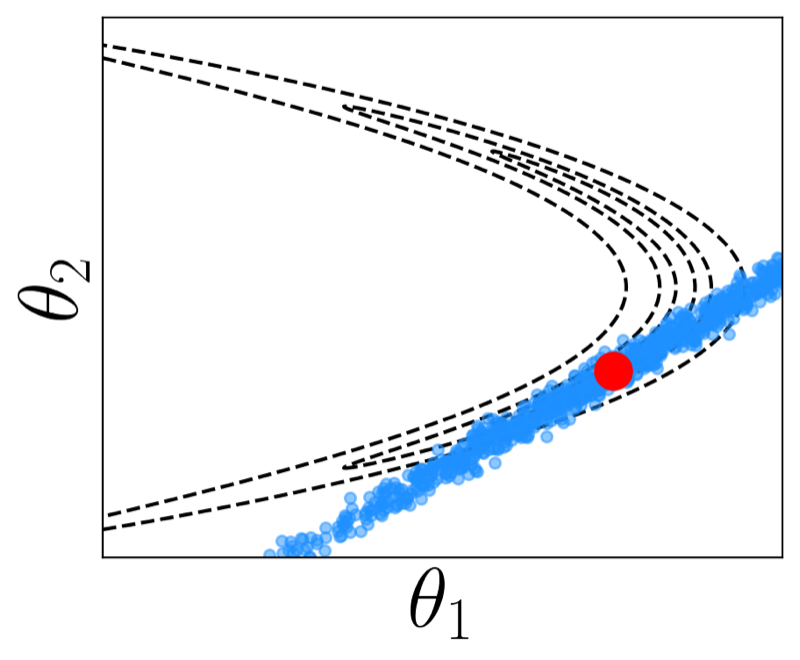
\includegraphics[width=0.38\textwidth, valign=m]{figs/paper1/h_banana_euclidean.png} & 
        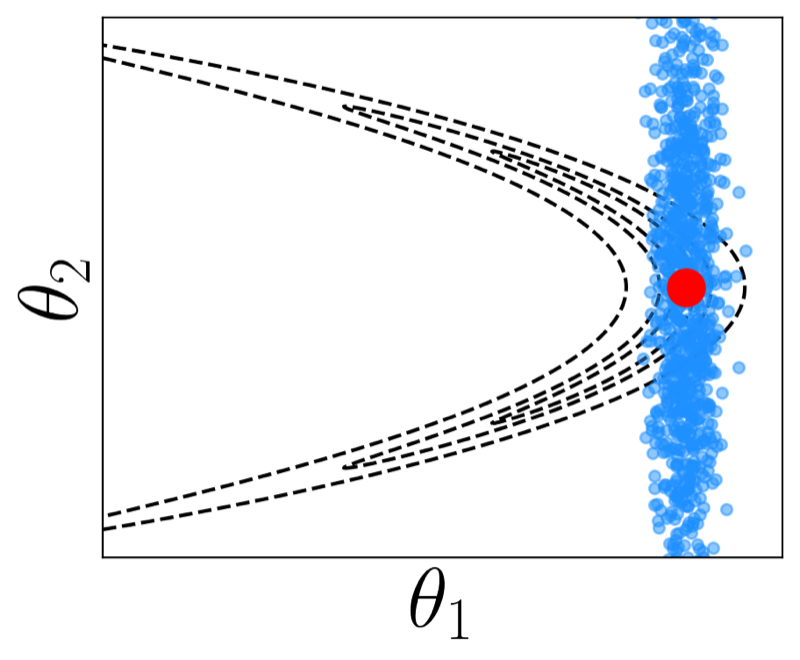
\includegraphics[width=0.38\textwidth, valign=m]{figs/paper1/f_banana_hausdorff_euclidean.png} \\
        RLA-B &
        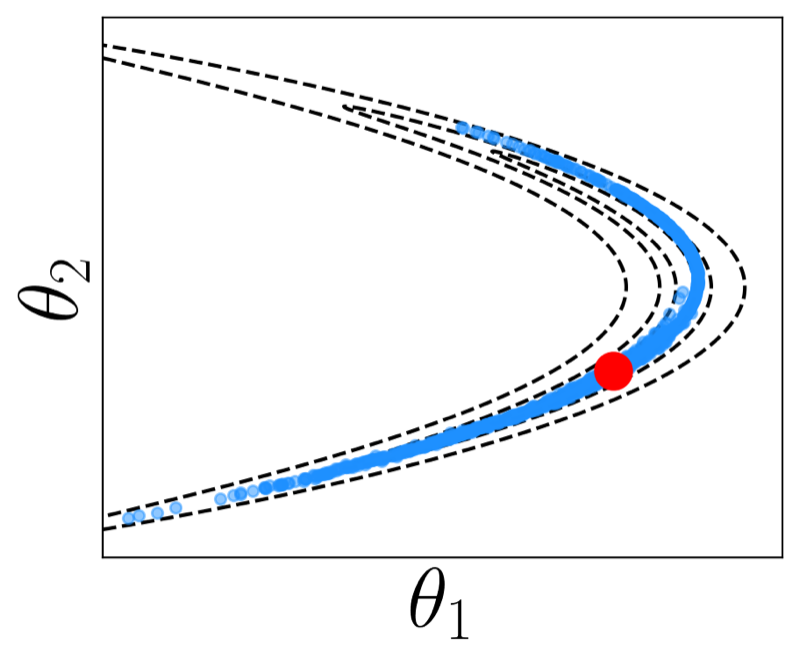
\includegraphics[width=0.38\textwidth, valign=m]{figs/paper1/h_banana_bergamin.png} & 
        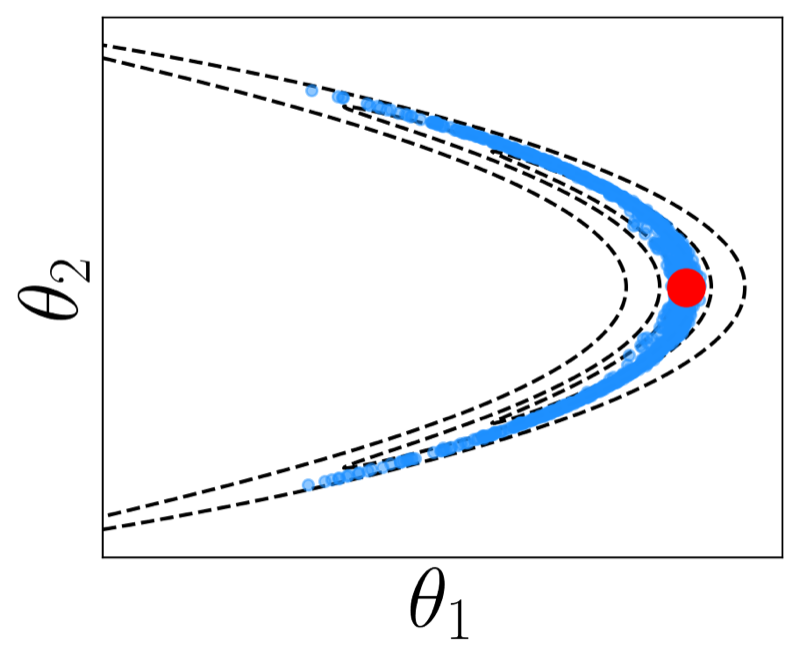
\includegraphics[width=0.38\textwidth, valign=m]{figs/paper1/f_banana_hausdorff_bergamin.png} \\
        RLA-BLog &
        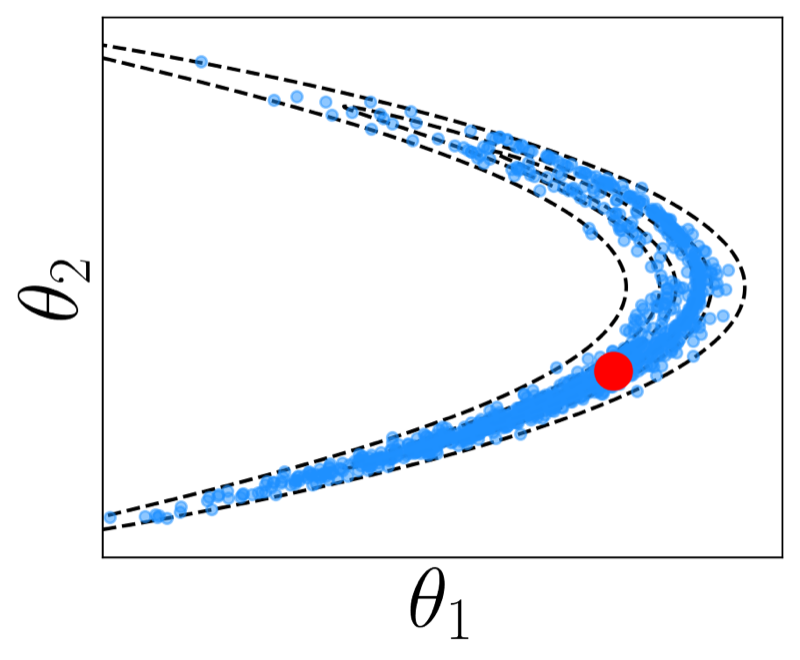
\includegraphics[width=0.38\textwidth, valign=m]{figs/paper1/h_banana_monge.png} & 
        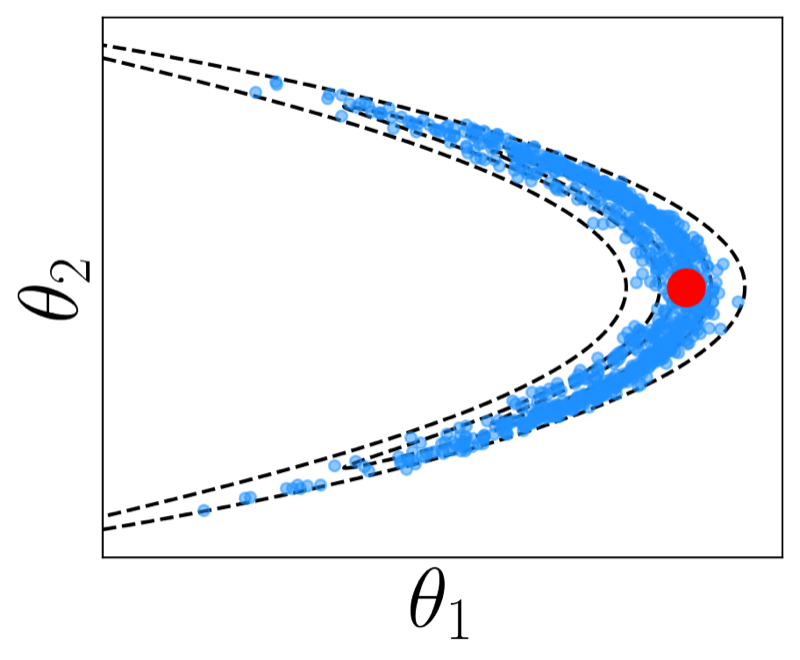
\includegraphics[width=0.38\textwidth, valign=m]{figs/paper1/f_banana_hausdorff_monge.png} \\
        RLA-F &
        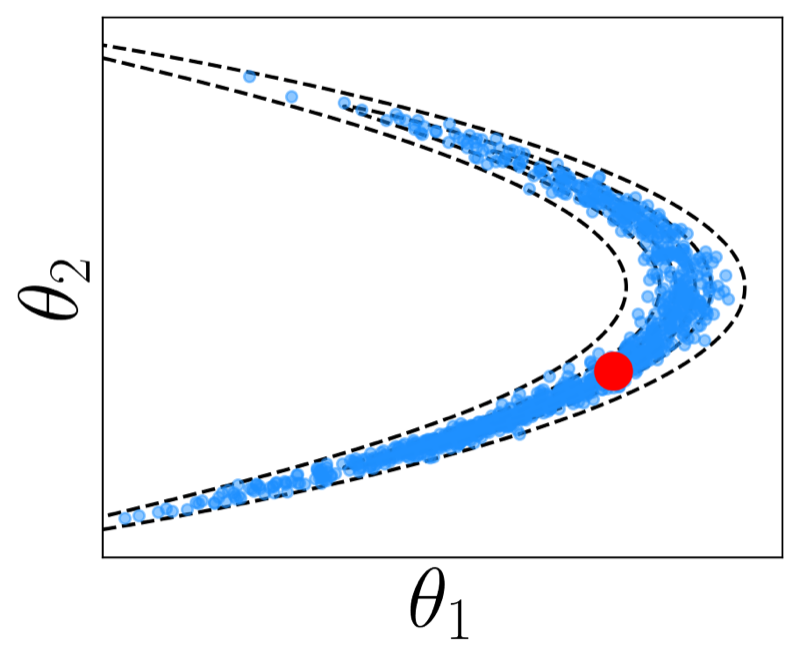
\includegraphics[width=0.38\textwidth, valign=m]{figs/paper1/h_banana_fisher.png} & 
        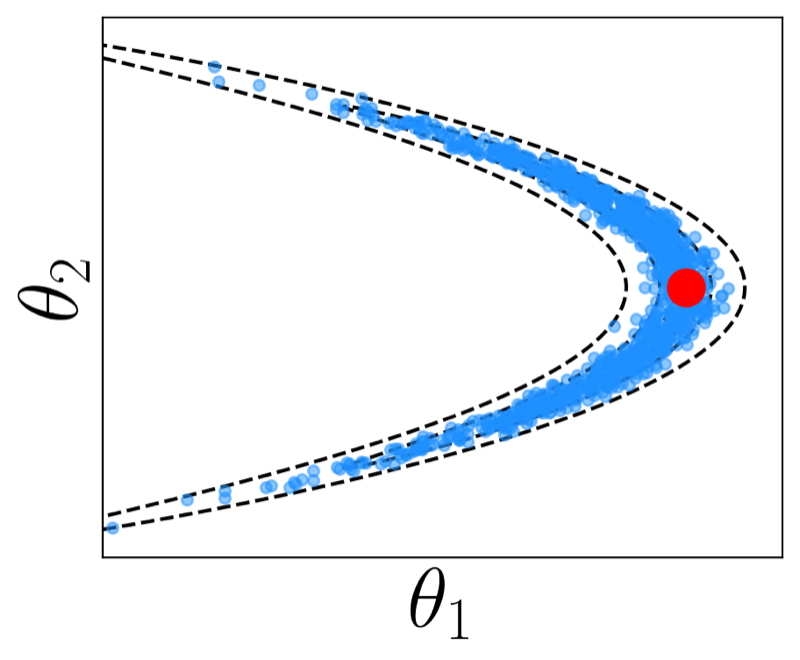
\includegraphics[width=0.38\textwidth, valign=m]{figs/paper1/f_banana_hausdorff_fisher.png}         
    \end{tabular}
    \caption{Comparison of Euclidean and Hausdorff MAP estimates. The red points are the Euclidean or Hausdorff MAP, and samples are scatter points in blue. The Euclidean metric (ELA) does not capture the geometry. The Monge metric is narrow without the logarithm map adjustment (RLA-B). The Fisher metric(RLA-F) is the most accurate with Hausdorff MAP. }
    \label{fig:banana}
\end{figure}


\paragraph{Efficiency of the approximation}
The second experiment considers Bayesian logistic regression on several benchmark data sets, both with standardized inputs and with raw inputs. The Fisher metric includes the Hessian of the prior as in Equation~\ref{eq:fisher_w_prior}. Table~\ref{tbl:lr} reports the Wasserstein distance to reference samples obtained with NUTS and the average number of log-density evaluations per sample.  The main takeaway is that 
RLA-F is more efficient in integration steps (geodesics are easier to integrate) and is more accurate than the Euclidean and Monge metric variants. 
\begin{table*}
	\centering
        \resizebox{\textwidth}{!}{
		\begin{tabular}{|l|l|l|l|l|l|l|l|l|}
			\hline
			 & & \multicolumn{1}{|c|}{ELA} & \multicolumn{2}{|c|}{RLA-B} & \multicolumn{2}{|c|}{RLA-BLog} & \multicolumn{2}{|c|}{RLA-F} \\
			\hline
			 & data & $\mathcal{W}$ & $\mathcal{W} \downarrow$ & $T$ & $\mathcal{W} \downarrow$ & $T$ & $\mathcal{W} \downarrow$ & $T$ \\
			\hline
			\multirow{5}{1em}{\centering\rotatebox[origin=c]{90}{stand.}}&Ripl & $0.106 \pm 0.004$ & $0.236 \pm 0.001$ & 29.7 & $0.16 \pm 0.065$ & 45.2 & $\textbf{0.064} \pm 0.002$ & \textbf{12.2} \\
			\cline{2-9}
			&Pima & $0.149 \pm 0.0$ & $0.274 \pm 0.0$ & 41.7 & $0.21 \pm 0.007$ & 78.5 & $\textbf{0.147} \pm 0.0$ & \textbf{12.2} \\
			\cline{2-9}
			&Hear & $0.529 \pm 0.001$ & $0.649 \pm 0.0$ & 40.2 & $1.154 \pm 0.189$ & 71.6 & $\textbf{0.514} \pm 0.0$ & \textbf{13.2} \\
			\cline{2-9}
			&Aust & $0.441 \pm 0.001$ & $0.522 \pm 0.001$ & 51.5 & $0.745 \pm 0.203$ & 79.1 & $\textbf{0.417} \pm 0.001$ & \textbf{18.0} \\
			\cline{2-9}
			&Germ & $0.388 \pm 0.001$ & $0.431 \pm 0.0$ & 58.4 & $0.676 \pm 0.1$ & 104.0 & $\textbf{0.387} \pm 0.0$ & \textbf{14.2} \\
			\hline
			\multirow{5}{1em}{\centering\rotatebox[origin=c]{90}{raw}}&Ripl & $0.437 \pm 0.017$ & $0.489 \pm 0.012$ & 30.2 & $0.554 \pm 0.253$ & 45.0 & $\textbf{0.247} \pm 0.012$ & \textbf{12.7} \\
			\cline{2-9}
			&Pima & $0.21 \pm 0.01$ & $0.294 \pm 0.004$ & 5632.9 & $0.216 \pm 0.014$ & 1690.4 & $\textbf{0.112} \pm 0.008$ & \textbf{15.4} \\
			\cline{2-9}
			&Hear & $0.842 \pm 0.026$ & $0.96 \pm 0.012$ & \textit{7868.2} & $0.898 \pm 0.029$ & \textit{3161.1} & $\textbf{0.644} \pm 0.012$ & \textbf{17.9} \\
			\cline{2-9}
			&Aust & $0.454 \pm 0.004$ & $0.455 \pm 0.01$ & \textit{18513.8} & $0.467 \pm 0.005$ & \textit{12298.6} & $\textbf{0.378} \pm 0.005$ & \textbf{18.0} \\
			\cline{2-9}
			&Germ & $0.846 \pm 0.002$ & $0.92 \pm 0.003$ & 3545.9 & $0.898 \pm 0.003$ & 2985.5 & $\textbf{0.823} \pm 0.001$ & \textbf{17.8} \\
			\hline
		\end{tabular}
        }	
	\caption{Logistic regression results as $\text{mean} \pm \text{std}$. Bold font indicates the best method. Italic font indicates the integrator reached maximum number of steps in at least one run. $\mathcal{W}$ indicates the 1-Wasserstein distance to NUTS samples while $T$ indicates the average number of function evaluations for one sample. For all evaluation metrics smaller is better.}
	\label{tbl:lr}
\end{table*}





\section{Case study II: geodesic slice sampling} \label{sec:geodesic_slice}
This case study uses the geometric tools from Section~\ref{sec:geometric_tools} in an MCMC sampling method.  In Section~\ref{sec:slice_sampling} we introduced  hit-and-run slice sampling that does slice sampling along Euclidean straight lines,  geodesic slice sampling from Paper~II keeps the same logic but replaces the straight lines by the geodesics induced by a metric choice. This change allows for MCMC sampling of distributions with strong curvature, multimodality or both.  

\paragraph{Geodesic slice sampling}
Our method builds on \citet{durmus2026geodesic}, who introduced geodesic slice sampling  over manifolds with closed form geodesics (e.g the sphere, torus, hyperbolic space,...). Paper~II extends this method to distributions defined on $\mathbb{R}^D$ with generic metric tensors $\mathbf{G}(\boldsymbol{x})$. Our method is metric-agnostic geodesic slice sampling (MAGSS).

In Euclidean hit-and-run slice sampling one first samples a random velocity $\boldsymbol{v}$ and performs univariate slice sampling on the straight line passing through the current state $\boldsymbol{x}$. Our method replaces the straight line 
$\boldsymbol{x} + t \boldsymbol{v}$ with the geodesic generated by the exponential map $\operatorname{Exp}_{\boldsymbol{x}}(t\boldsymbol{v})$, the target density $p(\boldsymbol{x})$ with the Hausdorff density $p_{\mathcal{H}}(\boldsymbol{x})$ and the Euclidean sphere $\mathbb{S}^{D-1}$ with the Riemannian sphere $\mathbb{S}^{D-1}_{\mathbf{G}}$  (see Table~\ref{tab:slice_compare}). Denote by  $\hat{\gamma}_{\boldsymbol{x},\boldsymbol{v}}(t)$ the numerical solution of the geodesic equations with initial conditions $\boldsymbol{x},\boldsymbol{v}$ for time $t$. Algorithm~\ref{alg:gss} shows the Geodesic Slice Sampling procedure.

\paragraph{Choice of metric}
Similar to Riemannian Laplace, the main modeling decision is the choice of Riemannian metric. For targets with strong local curvature, the Fisher, Monge and generative metrics can make geodesics better aligned with the shape of the density, with tradeoffs in the computational speed.

For multimodal targets, the inverse Monge and inverse generative metrics play a different role: they increase Euclidean speed in low-density regions and might be able to bridge between different modes, as discussed in Observations~\ref{obs:invmonge} and~\ref{obs:invgen}. In this sense, the same sampler can be adapted either to local geometry or to global mode exploration by changing only the metric tensor (as shown in Figure~\ref{fig:metric_visualization}). 
The Monge and generative metrics depend on hyperparameters. 
A limitation of our method is that there is no default value for these metric-parameters, some problems might allow for computation of a validation statistic for selection but no general value is optimal.


\paragraph{Meta-sampler} Paper II also considers a simple meta-sampler that alternates between geodesic slice sampling moves and local MCMC updates (e.g. MALA). The purpose of this combination is to use MAGSS with the inverse metrics for global transitions and the local Markov chain for exploration within each mode. This is particularly useful when the target is both multimodal and locally has high curvature. This is denoted by Meta-MAGSS. 



\begin{table}[t]
\centering
\small
\begin{tabular}{lll}
\toprule
 & Euclidean & Riemannian \\
\midrule
Slice level 
& $s \sim \mathrm{Unif}\!\bigl(0, p(\boldsymbol{x}^{(n)})\bigr)$
& $s \sim \mathrm{Unif}\!\bigl(0, \textcolor{mycolor}{p_{\mathcal{H}}}(\boldsymbol{x}^{(n)})\bigr)$ \\

Velocity 
& $\boldsymbol{v}^{(n)} \sim \mathrm{Unif}\!\bigl(\mathbb{S}^{D-1}(\boldsymbol{x}^{(n)})\bigr)$
& $\boldsymbol{v}^{(n)} \sim \mathrm{Unif}\!\bigl(\textcolor{mycolor}{\mathbb{S}^{D-1}_{\mathbf{G}}}(\boldsymbol{x}^{(n)})\bigr)$ \\

Slice sampling on 
& $\gamma_{\boldsymbol{x}^{(n)},\boldsymbol{v}^{(n)}}(t) = \boldsymbol{x}^{(n)} + t\boldsymbol{v}^{(n)}$
& $\textcolor{mycolor}{{\gamma}}_{\boldsymbol{x}^{(n)},\boldsymbol{v}^{(n)}}(t) 
= \textcolor{mycolor}{\operatorname{Exp}_{\boldsymbol{x}^{(n)}}}(t\boldsymbol{v}^{(n)})$ \\

\bottomrule
\end{tabular}
\caption{Comparison of Euclidean and Riemannian slice sampling components. Red highlights indicate the Riemannian modifications.}
\label{tab:slice_compare}
\end{table}



\begin{algorithm}[t]
    \caption{Geodesic slice sampling, producing $N$ samples $\boldsymbol{x}^{(n)}$.}    
	    \begin{algorithmic}[1]        
	    \Require Initial $\boldsymbol{x^{(0)}}$, metric $\mathbf{G}$ and parameters $m\in \mathbb{N}$, $w\ge 0$	        
	        \For{$n \leftarrow 0\dots N-1$}     
                \State Sample $s \sim \mathrm{Unif}(0, p_{\mathcal{H}}(\boldsymbol{x}^{(n)}))$ and $\boldsymbol{v}^{(n)} \sim \textrm{Unif}(\mathbb{S}_{\mathbf{G}}^{D-1}(\boldsymbol{x}^{(n)}))$
	            \State Obtain $(\ell, r) = \text{Step-out}_{w,m}(s, \hat{\gamma}_{\boldsymbol{x}^{(n)}, \boldsymbol{v}^{(n)}})$
	            \State Sample $t^* = \text{Shrink}_{\ell,r}(s, \hat{\gamma}_{\boldsymbol{x}^{(n)}, \boldsymbol{v}^{(n)}} )$
                \State Push-forward $\boldsymbol{x}^{(n+1)} \gets \hat{\gamma}_{\boldsymbol{x}^{(n)}, \boldsymbol{v}^{(n)}} (t^*)
                $
	        \EndFor
	\end{algorithmic}
	\label{alg:gss}
\end{algorithm}



\subsection*{Empirical evaluation}
The empirical evaluation compares parallel tempering (PT; \citealp{Latuszynski2025}), the diffusion Gibbs sampler (DiGS; \citealp{Chen2024}), and metric-agnostic geodesic slice sampling (MAGSS). We highlight some of the experiments from Paper~II. The objective of the experiments is to study our method on curved distributions and multimodal distributions, comparing the accuracy and running time against the alternatives. 

The first experiment shows MAGSS performance on curved target distributions. The second experiment compares the mode exploration of the methods on a highly multimodal target distribution modeling the Allen-Cahn field system. The third experiment studies the effect of the numerical integrator on our method. Paper~II gives the full description of the experimental setup and further analysis. 


\paragraph{Curved target distributions}
We consider the  Funnel, Rosenbrock and Squiggle target distributions with strong curvature from Section~\ref{sec:curved}. Figure~\ref{fig:toydistdims} shows the empirical 1-Wasserstein distance to reference samples from the distributions for dimensions $2,4,..2^8$. The Fisher metric produces the highest quality samples, but becomes computationally too expensive as can be seen by the cut-off in the lines, the Monge metric produces good results on Rosenbrock and Squiggle distributions. DiGS, PT and NUTS struggle exploring the curved regions of the space and are less accurate, note that DiGS uses the local MCMC  Metropolis-adjusted Langevin algorithm (MALA), a Riemannian version could be used instead to enhance exploration of the curved regions as an improvement to the method. The values of the hyperparameters of the Monge and generative metrics are $\alpha^2, \lambda=1$. 
We use the step-size value $w = 3$ and max iterations $m = 8$ in MAGSS.
DiGS uses a single noise scale of $1$ and NUTS and MALA (inside DiGS) use a stepsize of $0.1$. 

\begin{figure}[t]
    \centering
    \begin{minipage}{0.32\textwidth}
        \centering
        {Funnel}\\
        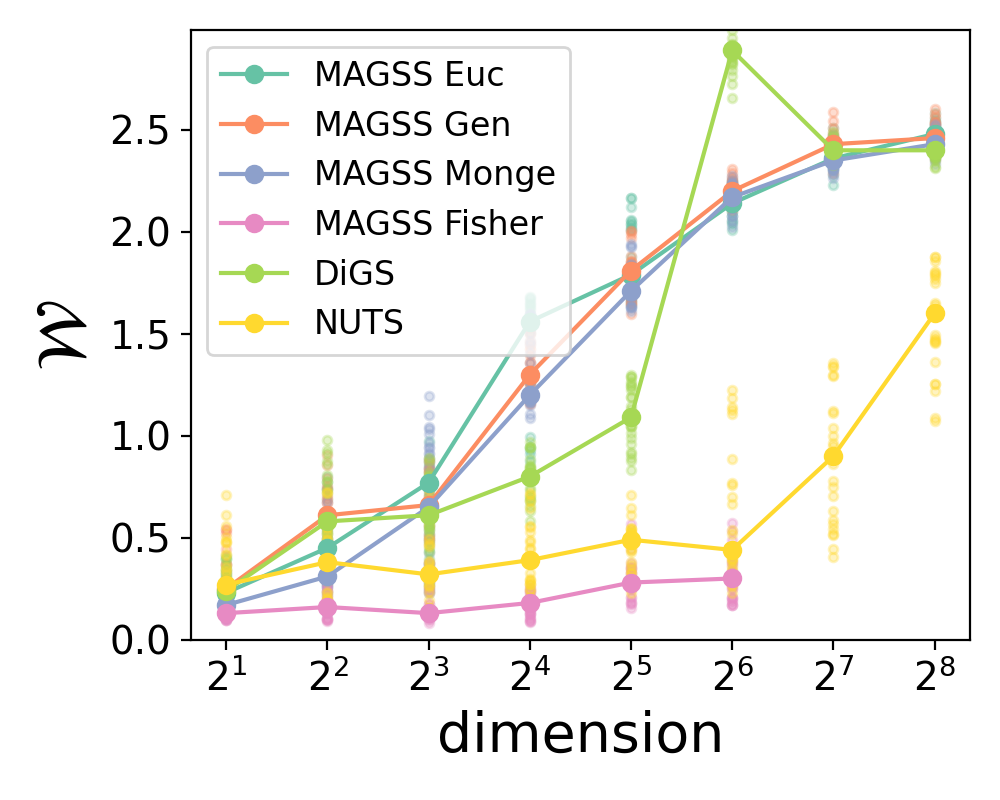
\includegraphics[width=\textwidth]{figs/paper2/rebutal/funnel_dims.png}
    \end{minipage}
    \hfill
    \begin{minipage}{0.32\textwidth}
        \centering
        {Rosenbrock}\\
        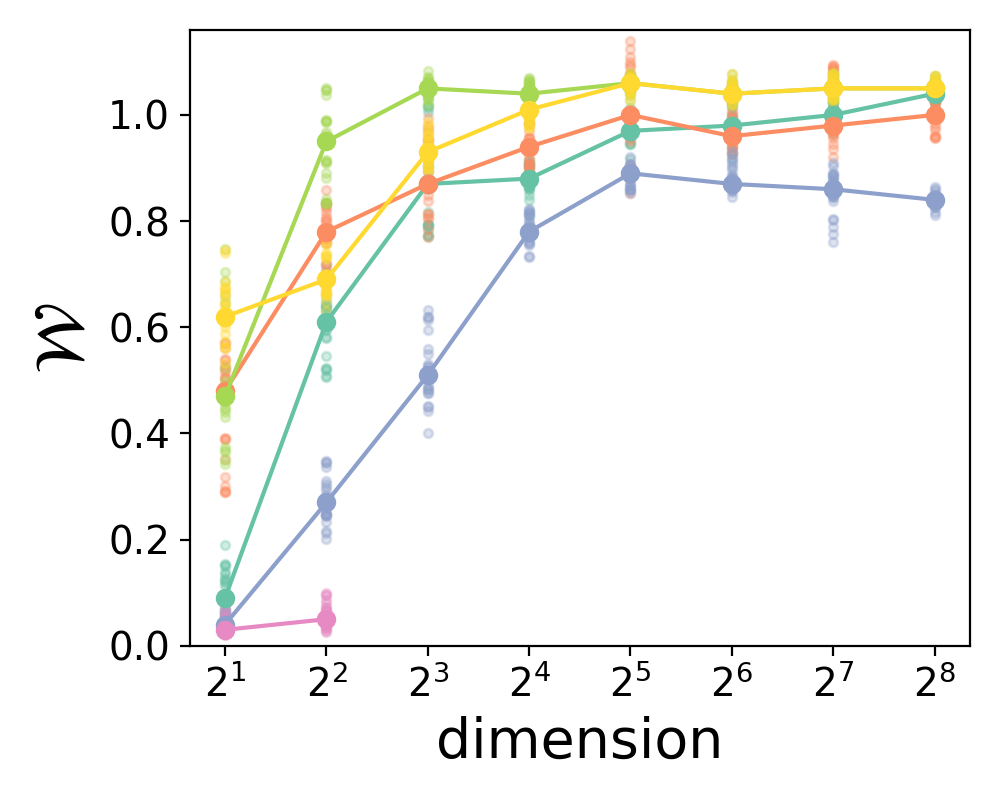
\includegraphics[width=\textwidth]{figs/paper2/rebutal/rosenbrock_dims.png}
    \end{minipage}
    \hfill
    \begin{minipage}{0.32\textwidth}
        \centering
        {Squiggle}\\
        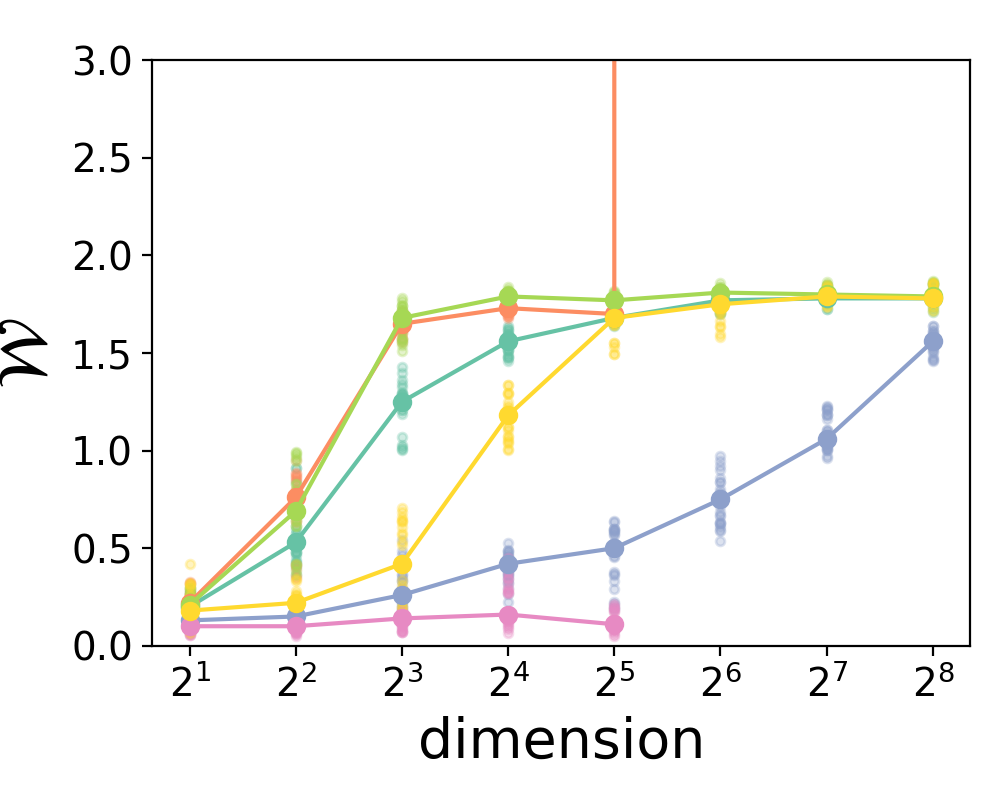
\includegraphics[width=\textwidth]{figs/paper2/rebutal/squiggle_dims.png}
    \end{minipage}
    \caption{Univariate sampling accuracy on different choice of Riemannian metric (1-Wasserstein distance, lower is better) for targets of varying dimensionality. The medians over 5 runs are connected with a line.}
    \label{fig:toydistdims}
\end{figure}

\paragraph{Highly multimodal target}
We consider the Allen-Cahn field system which has $2^D$ modes with $D=16$. This model has two global modes at $\boldsymbol{x} = \pm\boldsymbol{1}$, and multiple local modes at values $\boldsymbol{x} = (\pm 1,.., \pm 1)$. Table~\ref{tab:phifour} shows the results of the different sampling methods. 
Since there is no access to reference samples, we compute the Kernel Stein Discrepancy, but it is not trustworthy since it does not account for multimodality, the table also reports the percentage of samples such that $x_8\geq 0$ to see if the method was stuck on a single mode and the running time in seconds. MAGSS and DiGS are one order of magnitude slower than PT since they both rely on numerical integration.
Figure~\ref{fig:fieldsystem} shows that MAGSS explores the global and local modes, jumping the most frequently in between, while PT explores only the global modes and DiGS collapses to a single mode. A log-10 grid of parameters $\alpha^2, \lambda$ was tried, selecting the value based on the jump percentage. The inner sampler MALA stepsize was tuned to obtain an acceptance rate of approximately $60\%$. DiGS used $1000$ interpolation levels, ranging from $10^{-5}$ to $1-10^{-5}$. 
PT used $200$ temperatures on a geometric scale, with the smallest inverse temperature set to $10^{-5}$.

\begin{table}[t]
    \centering
    \caption{Allen-Cahn system model.}
\begin{tabular}{lllll}
\toprule
sampler &  KSD V-stat & $x_8>0$ & t(s) \\
\midrule
PT &   $0.13\pm0.04$ & $0.35$ & 6 \\
DiGS &   $0.13\pm0.05$ & $0.0$ & 157 \\
Meta-MAGSS  & $2.98\pm0.7$ & $0.33$ & 32 \\
\bottomrule
\end{tabular}    
    \label{tab:phifour}
\end{table}

\begin{figure}[t]
    \centering
    \begin{minipage}{0.32\linewidth}
        \centering
        {DiGS}\\
        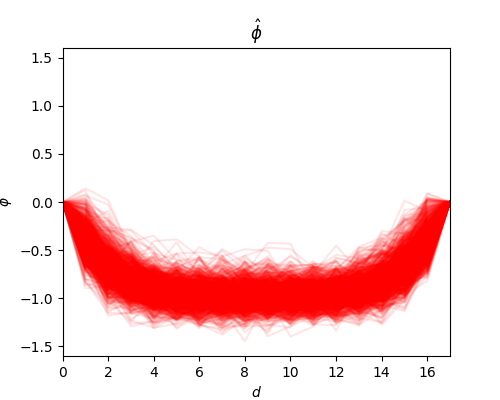
\includegraphics[width=\linewidth]{figs/paper2/rebutal/field_digs.png}
    \end{minipage}
    \hfill
    \begin{minipage}{0.32\linewidth}
        \centering
        {PT}\\
        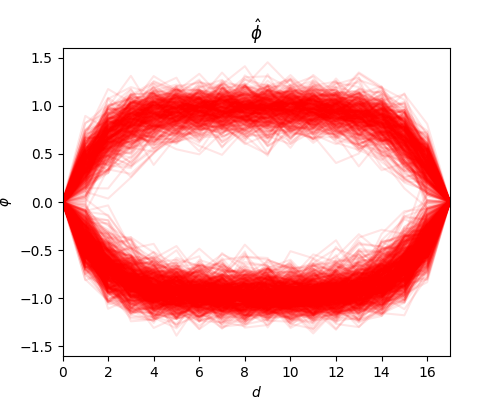
\includegraphics[width=\linewidth]{figs/paper2/rebutal/field_pt.png}
    \end{minipage}
    \hfill
    \begin{minipage}{0.32\linewidth}
        \centering
        {MAGSS}\\
        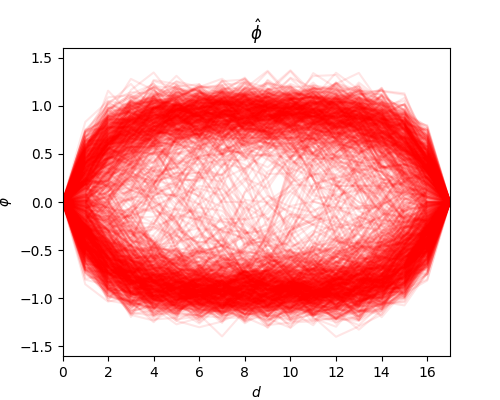
\includegraphics[width=\linewidth]{figs/paper2/rebutal/field_meta.png}
    \end{minipage}
    \caption{Samples from Allen-Cahn field system model with $2^{16}$ modes that zig-zag between $-1$ and $1$ on the y-axis over the $D=16$ values at the x-axis. Euclidean DiGS gets stuck in one mode, PT only explores two dominant modes with constant value over the x-axis, whereas Meta-MAGSS (inverse generative with $\lambda=10^{-6}$) explores also the modes that switch between the extremes.}
    \label{fig:fieldsystem}
\end{figure}


\paragraph{Sensitivity to the numerical integrator}
Here we study the effect of the choice of numerical integrator on a two dimensional 40-mode Gaussian  multimodal target for different values of $\alpha^2$ and $\lambda$ on a log-10 scale. We test integrators that are adaptive or fixed step-size and integrators with different order accurate solutions (see Figure~\ref{fig:gmm40}). 
The general trend is that as the inverse Monge and inverse generative metrics diverge from the Euclidean metric ($\alpha^2$ grows, $\lambda$ decreases), the system becomes stiffer and takes longer to integrate numerically. For the inverse Monge metric higher order and adaptive integrators work better, in practice we used Dopri5 in the other experiments because it has a good balance between the two. 
\begin{figure}[t]
    \centering
    \begin{minipage}{0.45\linewidth}
        \centering
        {Inverse generative metric}\\[0.5ex]
        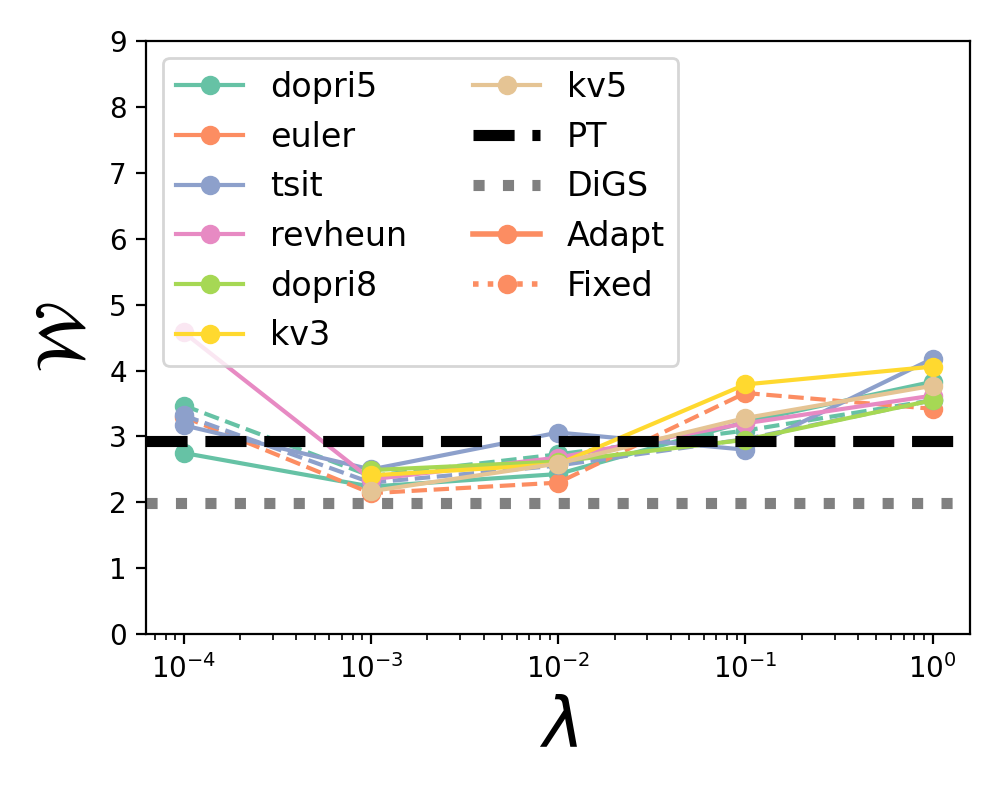
\includegraphics[width=\linewidth]{figs/paper2/gmm40/invGen_distances_mean_integrators.png}\\
        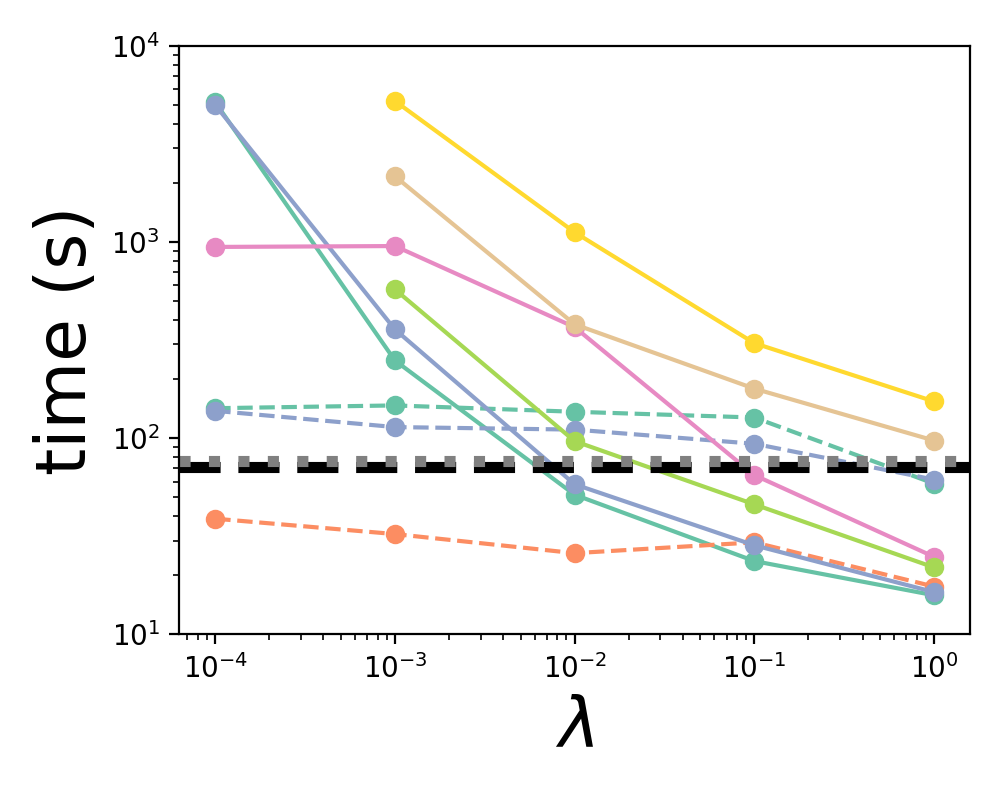
\includegraphics[width=\linewidth]{figs/paper2/gmm40/invGen_time_integrators.png}
    \end{minipage}
    \hfill
    \begin{minipage}{0.45\linewidth}
        \centering
        {Inverse Monge metric}\\[0.5ex]
        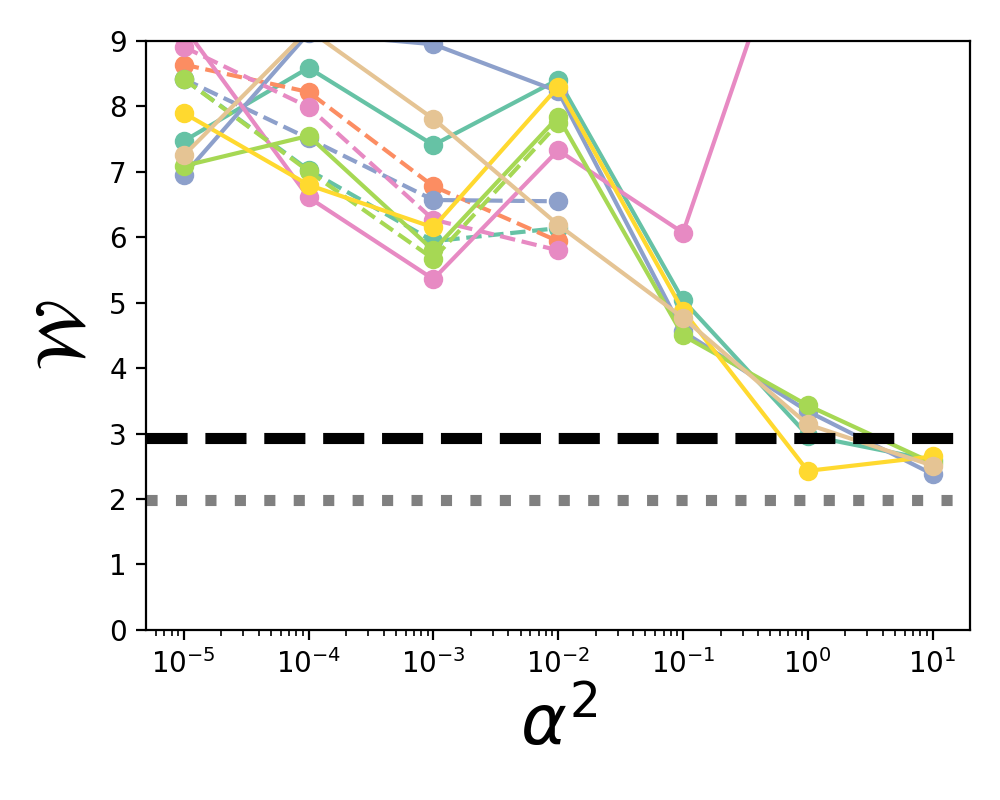
\includegraphics[width=\linewidth]{figs/paper2/gmm40/invMon_distances_mean_integrators.png}\\
        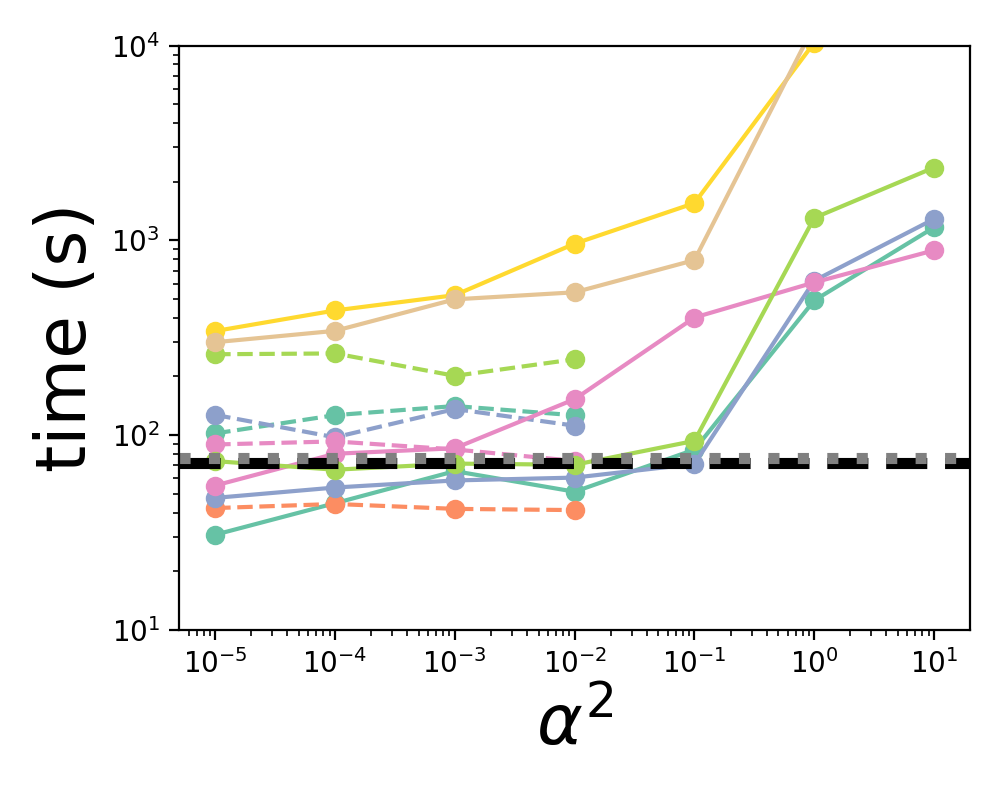
\includegraphics[width=\linewidth]{figs/paper2/gmm40/invMon_time_integrators.png}
    \end{minipage}
    \caption{Different numerical integrators for the 40 mode Gaussian mixture model. 
    The black dotted lines are PT and DiGS. Interpretation: the more the metric diverges from Euclidean (larger $\alpha^2$ and smaller $\lambda$) the more stiff the system is and the longer it takes to integrate. Generally, stiff systems benefit from adaptive integrators and produce more accurate samples.}
    \label{fig:gmm40}
\end{figure}

\chapter{Geometric Modeling of Discrete Data} \label{ch:simplex}

In this chapter we propose using the Aitchison geometry of the simplex space for modeling discrete data. The main idea is to represent simplex-valued distributions in Euclidean coordinates in a way that respects their natural geometry. We consider two applications of this idea: generative modeling of discrete data (Paper~III) and Gaussian process classification (Paper~IV).

We first introduce the Aitchison geometry and the simplex-to-Euclidean bijections that are used through the chapter. We then present stochastic interpolations that move discrete data from the boundary of the simplex to the interior, and provide theoretical guarantees for the recovery of the original discrete values. In the interior of the space we can use the bijections for modeling continuously in Euclidean coordinates, making the modeling compatible with Euclidean continuous methods. These ingredients are combined in two case studies: Simplex-to-Euclidean Flow Matching for generation of discrete data and Isometric Logratio Gaussian Processes for multiclass classification.


\paragraph{Motivation} We find that the Aitchison geometry provides for the  simplex, a geometry-aware representation that, combined with the stochastic interpolations, connects discrete modeling to known Euclidean methods. This makes existing Euclidean methods applicable to these tasks (generation and classification), providing a unified modeling framework that is exact and compatible with state-of-the-art Euclidean models while respecting the geometry of log proportions.

\section{Simplex-to-Euclidean Bijections}

We presented in Section~\ref{sec:discrete_data} the Fisher information geometry in the simplex, which is isomorphic to the positive orthant of the sphere. In this section and through the chapter, we instead use the Aitchison geometry of the simplex, because it provides a direct connection between the open simplex and Euclidean coordinates. We now introduce compositional data analysis which provides the building blocks for the Simplex-to-Euclidean bijections.

\subsection{Compositional Data Analysis}

\citet{Aitchison1981, Aitchison1982} introduced a geometry for the simplex that is not the Fisher information metric. This geometry is defined only on the interior of the simplex and the central idea is that information is carried by  the log-ratios of the components. Similarly to how the sigmoid function is a link function from binary classification to $\mathbb{R}$, the Aitchison geometry gives different choices of link functions from the open simplex to $\mathbb{R}^D$. The bijections make Euclidean modeling compatible with the simplex.

\paragraph{The geometry of the simplex}
Consider $K$-class categorical data $c\in\{1,\dots,K\}$, let $D:=K-1$.
The simplex and the open simplex are defined as
\begin{equation*}
    \Delta^{D}:=\{\boldsymbol{x}\in\mathbb{R}_{\ge 0}^{K}:\;\sum_{k=1}^{K}x_k=1\}, \quad 
    \mathring{\Delta}^{D}:=\{\boldsymbol{x}\in\mathbb{R}_{> 0}^{K}:\;\sum_{k=1}^{K}x_k=1\},
\end{equation*}
where only $D=K-1$ components are free, since one arbitrary component (for example the last one) is determined by the others as $x_K = 1-\sum_{d=1}^D x_d$.
The usual Euclidean operators are not closed on the simplex, for example the Euclidean sum of two vectors may fall outside the space. For this reason, \cite{Aitchison1986} defines perturbation (vector addition) and powering (scalar multiplication) that make the simplex a vector space. Define the normalization operation $\mathcal{C}(\boldsymbol{x}) := \boldsymbol{x}/\sum_{k=1}^{K} x_k$. For $\boldsymbol{x}, \boldsymbol{y}\in\mathring\Delta^D$ and $\lambda\in \mathbb{R}$, define
\begin{align*}
\textbf{perturbation} \quad
&\boldsymbol{x} \oplus \boldsymbol{y}
:= \mathcal{C}(x_1 y_1,\ldots, x_K y_K), \text{ and} \\
\textbf{powering} \quad
&\lambda \odot \boldsymbol{x}
:= \mathcal{C}(x_1^\lambda,\ldots, x_K^\lambda).
\end{align*}
Under these operations, $(\mathring\Delta^D, \oplus, \odot)$ is a vector space and the neutral element  is $\tfrac{1}{K}\boldsymbol{1}$ since $\boldsymbol x \oplus (\tfrac{1}{K}\boldsymbol{1}) = \boldsymbol x$. The vector space is an inner product space when given the Aitchison inner product defined as
\begin{equation*}
\langle \boldsymbol{x}, \boldsymbol{y} \rangle_A := \frac{1}{2K} \sum_{i,j=1}^{K} 
\log\frac{x_i}{x_j}\log\frac{y_i}{y_j}.
\end{equation*}
The norm of a vector is $\|\boldsymbol{x}\|_A = \sqrt{\langle \boldsymbol{x}, \boldsymbol{x} \rangle_A}$. The distance between two compositions is 
\begin{equation*}
    d_A(\boldsymbol x,\boldsymbol y) = 
    \|\boldsymbol{x} \ominus \boldsymbol{y}\|_A
= \sqrt{\frac{1}{2K}\sum_{i,j=1}^K
\left(\log\frac{x_i}{x_j}-\log\frac{y_i}{y_j}\right)^2 },
\end{equation*}
where $\boldsymbol{x} \ominus \boldsymbol{y} :=  \boldsymbol{x} \oplus  (-1 \odot\boldsymbol{y})$.

\paragraph{The simplex as embedded  Riemannian manifold}
The simplex can be viewed as an embedded manifold in $\mathbb{R}^K$. It is the intersection of the hyperplane $\sum_{k=1}^K x_k=1$ and the positive orthant. Because the hyperplane is flat, all tangent spaces are parallel and identified with the zero-sum linear space
\begin{equation*}
\mathbb{H}^{D}=\left\{\boldsymbol{z}\in\mathbb{R}^K:\sum_{i=1}^K z_i=0\right\}.
\end{equation*}
To give the open simplex a geometry, we use the center logratio map (CLR), which is a bijection between  $\mathring \Delta^D$ and the zero-sum hyperplane $\mathbb{H}^D$
\begin{equation*}
\begin{aligned}
    \operatorname{clr}: \mathring\Delta^D &\to \mathbb{H}^D, \quad
    \boldsymbol{x} \mapsto \boldsymbol{z}
    = \log \boldsymbol{x} - \frac{1}{K}\sum_{k=1}^{K} \log x_k \,\boldsymbol{1}, \text{ and} \\
    \operatorname{clr}^{-1}: \mathbb{H}^D &\to \mathring\Delta^D, \quad
    \boldsymbol{z} \mapsto \boldsymbol{x}
    = \mathcal{C} (\exp\boldsymbol{z}).
\end{aligned}
\end{equation*}
The image of the map lies in $\mathbb{H}^{D}$ because the components of $\operatorname{clr}(\boldsymbol{x})$ sum to zero, and the inverse map is usually known as the \emph{softmax}. In addition, the center logratio map is an isometry between $(\mathring\Delta^{D},\langle\cdot,\cdot\rangle_A)$ and $(\mathbb{H}^{D},\langle\cdot,\cdot\rangle_2)$, since the Aitchison norm and inner products are (after some algebraic manipulations)
\begin{align*}
\langle \boldsymbol{x}, \boldsymbol{y} \rangle_A &= 
\langle \operatorname{clr}(\boldsymbol{x}), \operatorname{clr}(\boldsymbol{y}) \rangle_2 
=\frac{1}{2K} \sum_{i,j=1}^{K} 
\log\frac{x_i}{x_j}\log\frac{y_i}{y_j}, \text{ and} \\
d(x,y)_A &= 
\| \operatorname{clr}(\boldsymbol{x})- \operatorname{clr}(\boldsymbol{y}) \|_2 
 = \sqrt{\frac{1}{2K}\sum_{i,j=1}^K
\left(\log\frac{x_i}{x_j}-\log\frac{y_i}{y_j}\right)^2 }.
\end{align*}
This means that the Aitchison geometry of the simplex is inherited from $\mathbb{H}^{D}$ via the center logratio map, thus the Riemannian metric is the pullback metric:
\begin{equation*}
    \mathbf{G}(\boldsymbol{x}) = \mathbf{J}_{\mathrm{clr}}(\boldsymbol{x})^\top\mathbf{J}_{\mathrm{clr}}(\boldsymbol{x}),
\end{equation*}
for $\mathbf{J}_{\mathrm{clr}}(\boldsymbol{x}) = \pdv{\operatorname{clr}(\boldsymbol{x})}{\boldsymbol{x}_{1:D}}$ where the Jacobian is computed with respect to the first $D$ coordinates because of the extra degree of freedom and $x_K =1- \sum_{d=1}^Dx_d$. The geodesics are computed by pulling back straight lines in $\mathbb{H}^D$
\begin{equation*}
    \gamma(t) = \operatorname{clr}^{-1}\bigl((1-t)\operatorname{clr}(\boldsymbol{x}) + t\operatorname{clr}(\boldsymbol{y})\bigr) = 
    \bigl((1-t)\odot \boldsymbol{x}\bigr) \oplus \bigl(t\odot \boldsymbol{y}\bigr).
\end{equation*}


\paragraph{Isometric Logratio}
The CLR map gives the simplex the Aitchison geometry, but the image of the map still lands in the constrained hyperplane $\mathbb{H}^D$. For practical modeling it is more convenient to work in ordinary Euclidean coordinates. The isometric logratio (ILR) map of \citet{Egozcue2003} achieves this by expressing CLR coordinates in an orthonormal basis of $\mathbb{H}^D$. This basis is given by the Helmert matrix $\mathbf{H}\in \mathbb{R}^{D\times K}$ \citep{Lancaster1965}, and the resulting bijection is
\begin{equation*}
    \varphi(\boldsymbol{x}) = \mathbf{H} \, \operatorname{clr}(\boldsymbol{x}).
\end{equation*}
The Helmert matrix has the property that $\mathbf{H}\boldsymbol{1} = \boldsymbol{0}$, then 
\begin{equation*}
\mathbf{H} \, \operatorname{clr}(\boldsymbol{x})
=
\mathbf{H} \log \boldsymbol{x}
-
\frac{1}{K}\sum_{k=1}^{K} \log x_k \,
\underbrace{\mathbf{H}\boldsymbol{1}}_{=\boldsymbol{0}}
=
\mathbf{H} \log \boldsymbol{x}.
\end{equation*}
The ILR map and its inverse are therefore
\begin{equation} \label{eq:ilr}
    \begin{aligned}
    \varphi: \mathring\Delta^{D} \to \mathbb{R}^{D},\quad  &\boldsymbol{x}\mapsto \boldsymbol{z}= \mathbf{H} \log \boldsymbol{x}, \text{ and} \\
    \varphi^{-1}:  \mathbb{R}^{D} \to \mathring\Delta^{D}, \quad &\boldsymbol{z}\mapsto \boldsymbol{x} = \mathcal{C}\left(\exp (\mathbf{H}^\top \boldsymbol{z} )\right).
    \end{aligned}
\end{equation}
This bijection is simpler because we can use the standard basis of the Euclidean space $\mathbb{R}^D$ along with the Euclidean inner product to model in the latent space while preserving the Aitchison geometry. The isometry is stated in Theorem~\ref{thm:isometry}, and the proof is omitted here. A visualization of the Aitchison geometry is in Figure~\ref{fig:fig1}, which shows the latent distribution and geodesic balls on both spaces.
\begin{figure}
    \centering
    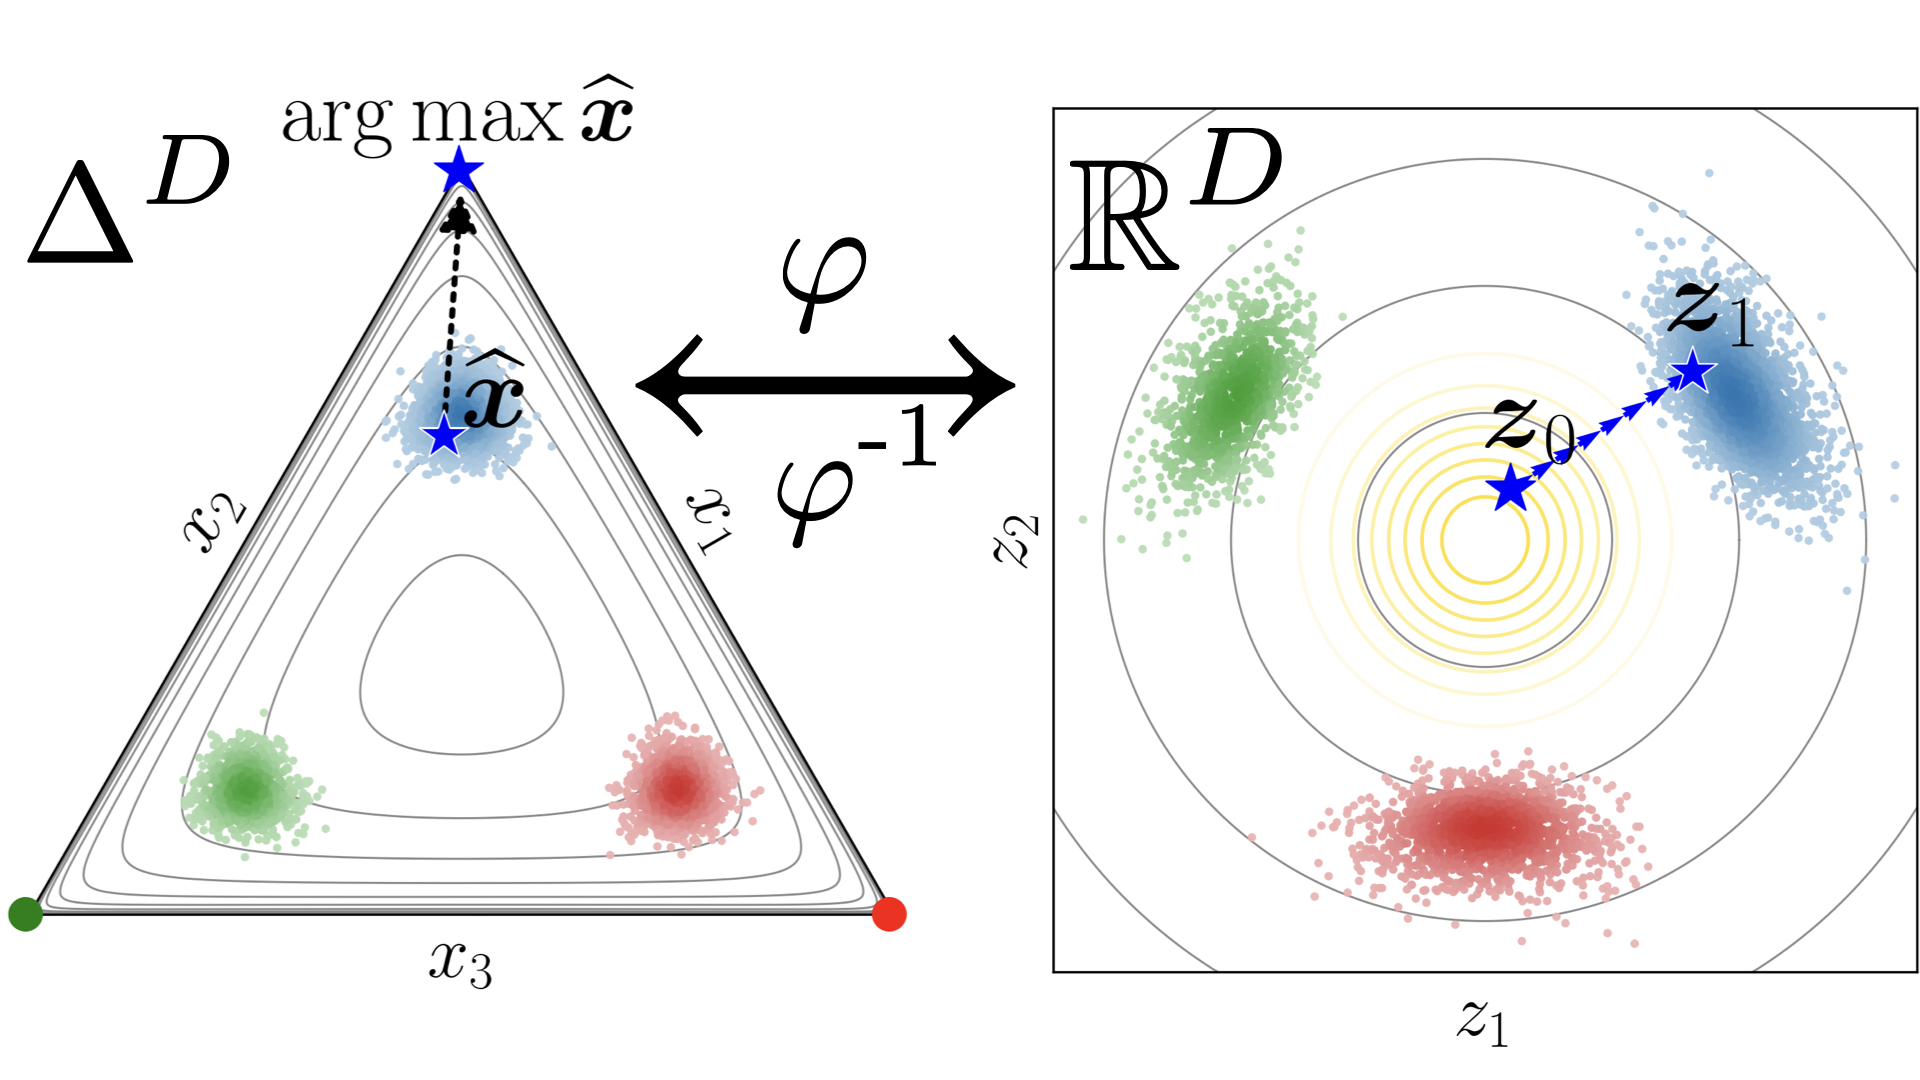
\includegraphics[width=0.8\linewidth]{figs/paper3/fig1.001.jpeg}
    \caption{Visual representation of the Aitchison geometry and Simplex-to-Euclidean Flow Matching.}
    \label{fig:fig1}
\end{figure}

\begin{theorem}[Isometry, \citep{Egozcue2003}]\label{thm:isometry}
Let $\langle\cdot,\cdot\rangle_A$ denote the Aitchison inner product on $\mathring \Delta^{D}$ and $\langle\cdot,\cdot\rangle_2$ the standard inner product on $\mathbb{R}^{D}$. For a Helmert matrix $\mathbf{H} \in\mathbb{R}^{D\times K}$, the ILR map satisfies
\begin{equation*}
    \langle \boldsymbol{x}, \boldsymbol{y} \rangle_A \,=\, \langle \varphi(\boldsymbol{x}), \varphi(\boldsymbol{y}) \rangle_2 \quad \forall \boldsymbol{x},\boldsymbol{y}\in \mathring\Delta^D,
\end{equation*}
and, in particular, the ILR map is an isometry between $(\mathring\Delta^{D},\langle\cdot,\cdot\rangle_A)$ and $(\mathbb{R}^{D},\langle\cdot,\cdot\rangle_2)$. 
\end{theorem}

The Riemannian metric in the tangent space of the open simplex is naturally defined by the pullback of the transformation
\begin{equation*}
    \mathbf{G}(\boldsymbol{x}) = \mathbf{J}_{\varphi}(\boldsymbol{x})^\top\mathbf{J}_{\varphi}(\boldsymbol{x}),
\end{equation*}
with $\mathbf{J}_{\varphi}(\boldsymbol{x}) = \pdv{\varphi(\boldsymbol{x})}{\boldsymbol{x}_{1:D}}$ is computed with respect to the standard Euclidean basis. 
The Aitchison geodesic between $\boldsymbol{x}$ and $\boldsymbol{y}$ is computed through the pullback
\begin{equation*}
    \gamma(t) = \varphi^{-1}\bigl((1-t)\varphi(\boldsymbol{x}) + t\varphi(\boldsymbol{y})\bigr) = 
    \bigl((1-t)\odot \boldsymbol{x}\bigr) \oplus \bigl(t\odot \boldsymbol{y}\bigr).
\end{equation*}

\paragraph{Other simplex-to-Euclidean bijections}
\citet{Aitchison1980} and \citet{Aitchison1982} also introduced other logratio maps from the open simplex to Euclidean space. Two classical bijections are the additive logratio (ALR) and the multiplicative log ratio (MLR), defined as
\begin{align}
    \mathrm{alr}(\boldsymbol{x})_k &:=  \log\tfrac{x_k}{x_{K}}, \quad &\mathrm{alr}^{-1}(\boldsymbol{z}) =  \mathrm{softmax}([\boldsymbol{z},0]),\\
    \mathrm{mlr}(\boldsymbol{x})_k &:=  \log\tfrac{x_k}{1 - \sum_{i=1}^{k} x_{i}}, \quad
    &\mathrm{mlr}^{-1}(\boldsymbol{z})_k =  \frac{e^{z_k}}{\prod_{i=1}^k \big(1+e^{z_i}\big)}.
    \label{eq:alr}
\end{align}
Note that these maps, unlike ILR, depend on the order of the input and are not isometric to Euclidean space. They produce a different map for permutations of the entries.
Nevertheless, these maps are useful for reparametrization, for example the logistic-normal distribution \citep{Aitchison1980} is the push-forward distribution of a Gaussian over the additive logratio map.

\paragraph{Stick-breaking transform}
A simple centering adjustment improves MLR. MLR is not centered at the vector $\tfrac{1}{K}\boldsymbol{1} \in \Delta^D$, so it does not map the zero vector in $\mathbb{R}^D$ to $\tfrac{1}{K}\boldsymbol{1}$.
The stick-breaking (SB) fixes this by shifting the MLR map
\begin{equation}\label{eq:sb}
\begin{aligned}
\varphi : \mathring{\Delta}^{D} &\to \mathbb{R}^{D}, \quad
\boldsymbol{x} \mapsto \boldsymbol{z}, \quad
z_k = \mathrm{mlr}(\boldsymbol{x})_k - \log\!\left(\frac{1}{K - k}\right), 
\text{ and}
\\
\varphi^{-1} : \mathbb{R}^{D} &\to \mathring{\Delta}^{D}, \quad
\boldsymbol{z} \mapsto \boldsymbol{x}, \quad
\boldsymbol{x} = \mathrm{mlr}^{-1}(\boldsymbol{y}), \quad
y_k = z_k + \log\!\left(\frac{1}{K - k}\right).
\end{aligned}
\end{equation}
Unlike ILR, stick-breaking remains order-dependent and is not an isometry, but it is simple, numerically stable, and widely used in probabilistic modeling \citep{Carpenter2017}.

\subsection{Simplex stochastic interpolations}
The Aitchison geometry is defined  on the open simplex, but discrete observations lie on the boundary of the space. We therefore construct stochastic interpolations that move discrete labels into the interior during modeling while still allowing us to recover the original categories afterwards. Dirichlet based Gaussian process classification presented in Section~\ref{sec:gp}, use a deterministic interpolation in the simplex on the parameters of the Dirichlet distribution of the form $\lambda \boldsymbol{e}_k + (1-\lambda) \tfrac{1}{K}\boldsymbol 1$, for $\lambda\in (0,1)$. 

\paragraph{Dirichlet interpolation}
We first construct stochastic interpolations where the noise process is distributed in the simplex itself. Define the distinct $\arg\max$ regions
\begin{equation}    
    \mathcal{R}_k := \{ \boldsymbol{x}\in \mathring \Delta^{D} : x_k > x_j\ \forall j\neq k\}.
    \label{eq:interpolation}
\end{equation}
These regions partition the interior of the simplex up to zero measure ties ($x_k=x_j$ for $j\neq k$).
If the interpolated sample remains on the region $\mathcal{R}_k$ then the $\arg \max$ returns the original category before interpolation. For class label $c=k$ with one-hot representation $\boldsymbol{e}_k$ we define the stochastic interpolation
\begin{equation}
\boxed{
    {\boldsymbol{x}} = \lambda \boldsymbol{e}_k + (1-\lambda) \boldsymbol{\varepsilon}.
}
\end{equation}
The parameter $\lambda$ controls how far the sample is moved away from the boundary. 
Proposition~\ref{prop:interpolation} states that for $\lambda\geq 1/2$ the original category remains in $\mathcal{R}_k$ and is recovered via $c = \arg\max \boldsymbol{x}$ almost surely (see Figure~\ref{fig:lambda}).

The noise process can be any distribution over the simplex, we choose the symmetric Dirichlet noise distribution $\mathrm{Dir}(\alpha\boldsymbol{1})$ because it has a simple covariance structure in ILR coordinates. The latent ILR covariance is the same independent of the number of categories $K$. Let $\boldsymbol{z} = \varphi(\boldsymbol{x})$ under the ILR map, then
\begin{equation*}
\operatorname{Cov}(\boldsymbol{z})=\psi'(\alpha)\,\mathbf{I}_{D},
\end{equation*}
where $\psi'$ is the trigamma function \citep{Aitchison1986}. This is convenient and justifies using the same value of $\alpha$ for any number of categories. In practice we use $\alpha>1$, which concentrates the interpolation's mass near the mean of the distribution and away from the boundary of the simplex.

\begin{proposition}[Proposition 1, Paper III] \label{prop:interpolation}
\textbf{Dirichlet Interpolation:}
Let $\boldsymbol{c} = \boldsymbol{e}_k$ for some $k\in\{1,..,K\}$. Let ${\boldsymbol{x}} := \lambda \boldsymbol{c} + (1-\lambda) \boldsymbol{\varepsilon}$
where $\boldsymbol{\varepsilon} \sim \mathrm{Dir}(\boldsymbol{\alpha})$ with $\alpha_i > 0$.
If $\lambda > \tfrac{1}{2}$, then $\arg\max {\boldsymbol{x}} = \boldsymbol{c}$. For $\lambda = \tfrac{1}{2}$, this holds almost surely under the distribution of $\boldsymbol{\varepsilon}$.
\end{proposition}


\begin{figure}
    \centering    
    \begin{subfigure}{0.3\linewidth}
        \centering
        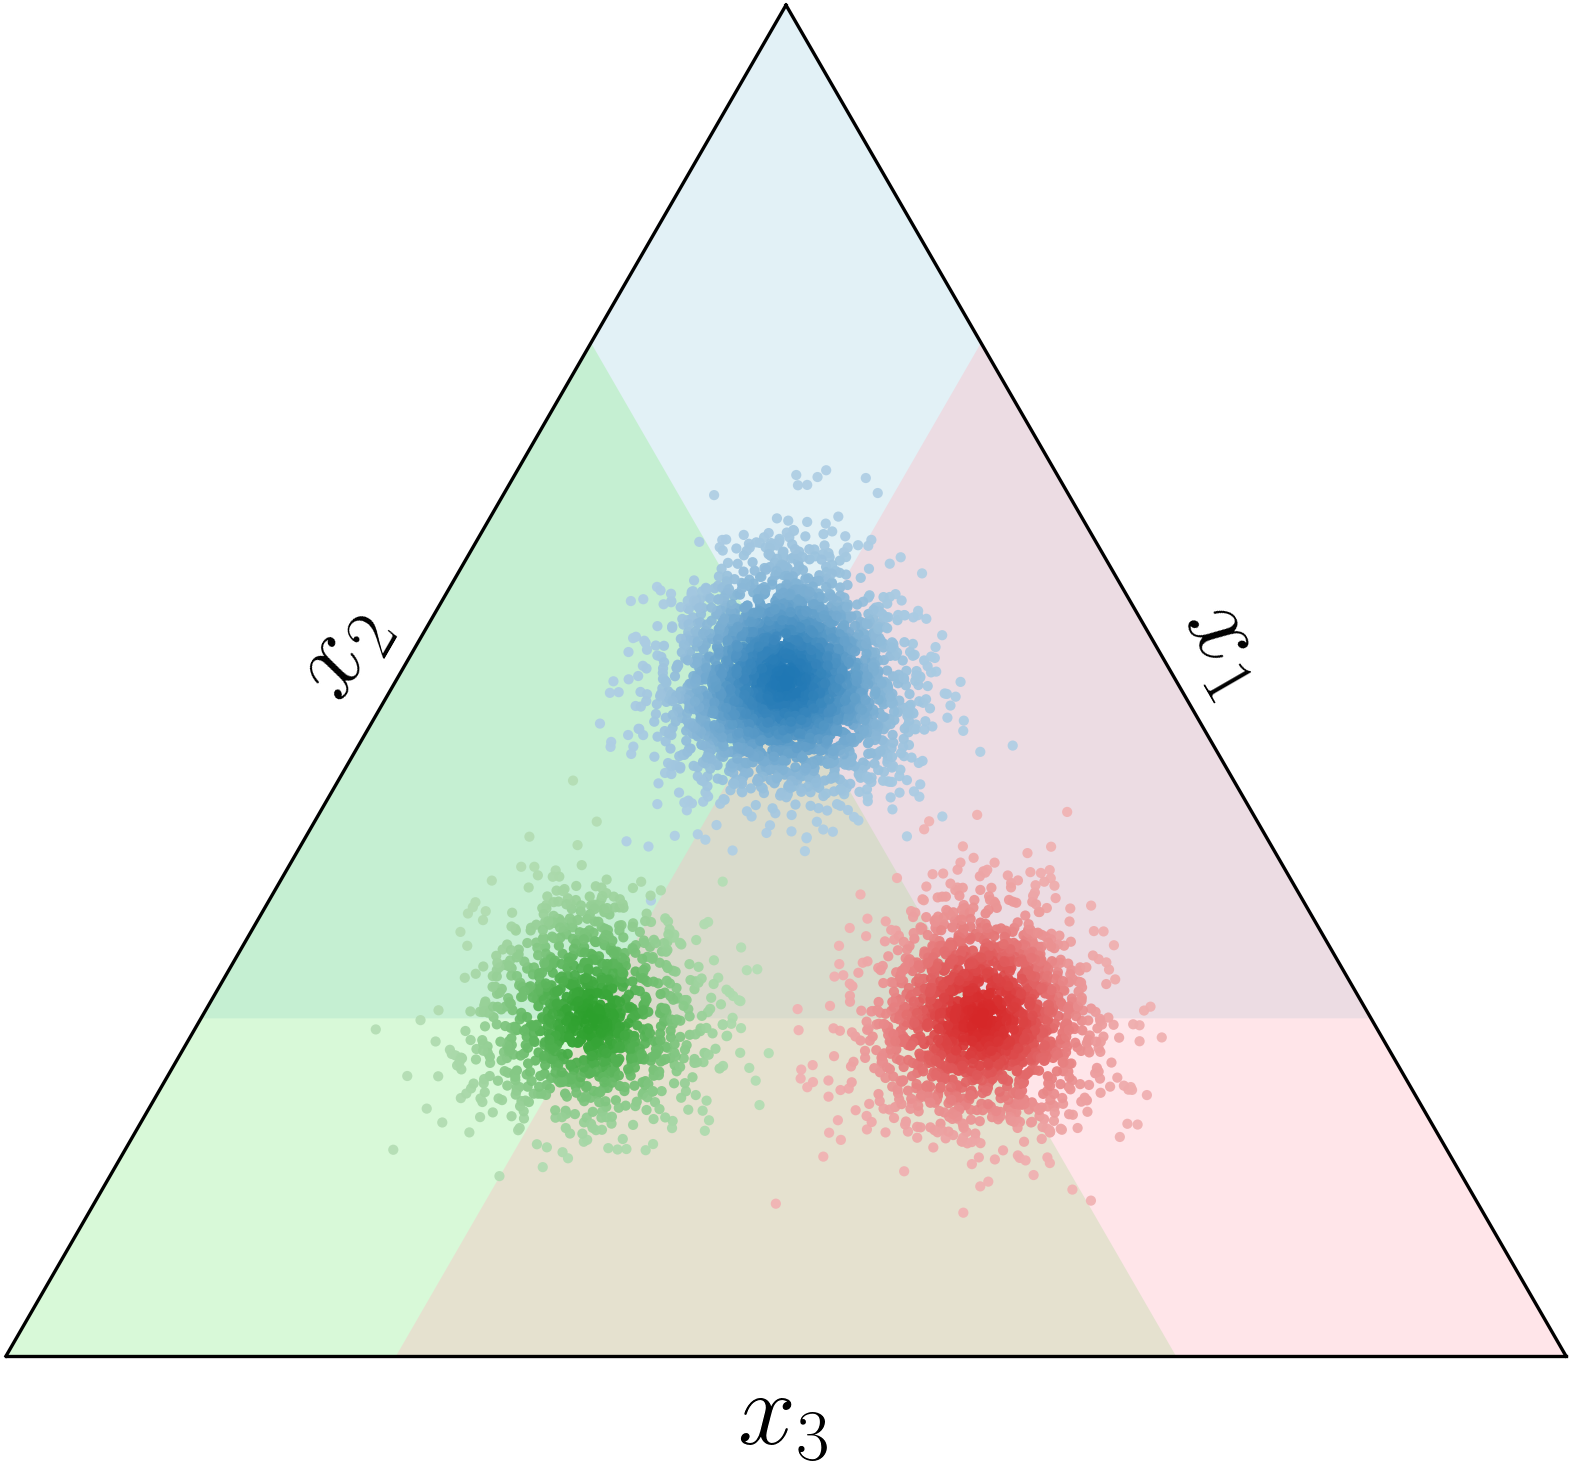
\includegraphics[width=\linewidth]{figs/paper3/lambd_0.25.png}
        \caption*{$\lambda=\tfrac{1}{4}$}
    \end{subfigure}
    \begin{subfigure}{0.3\linewidth}
        \centering
        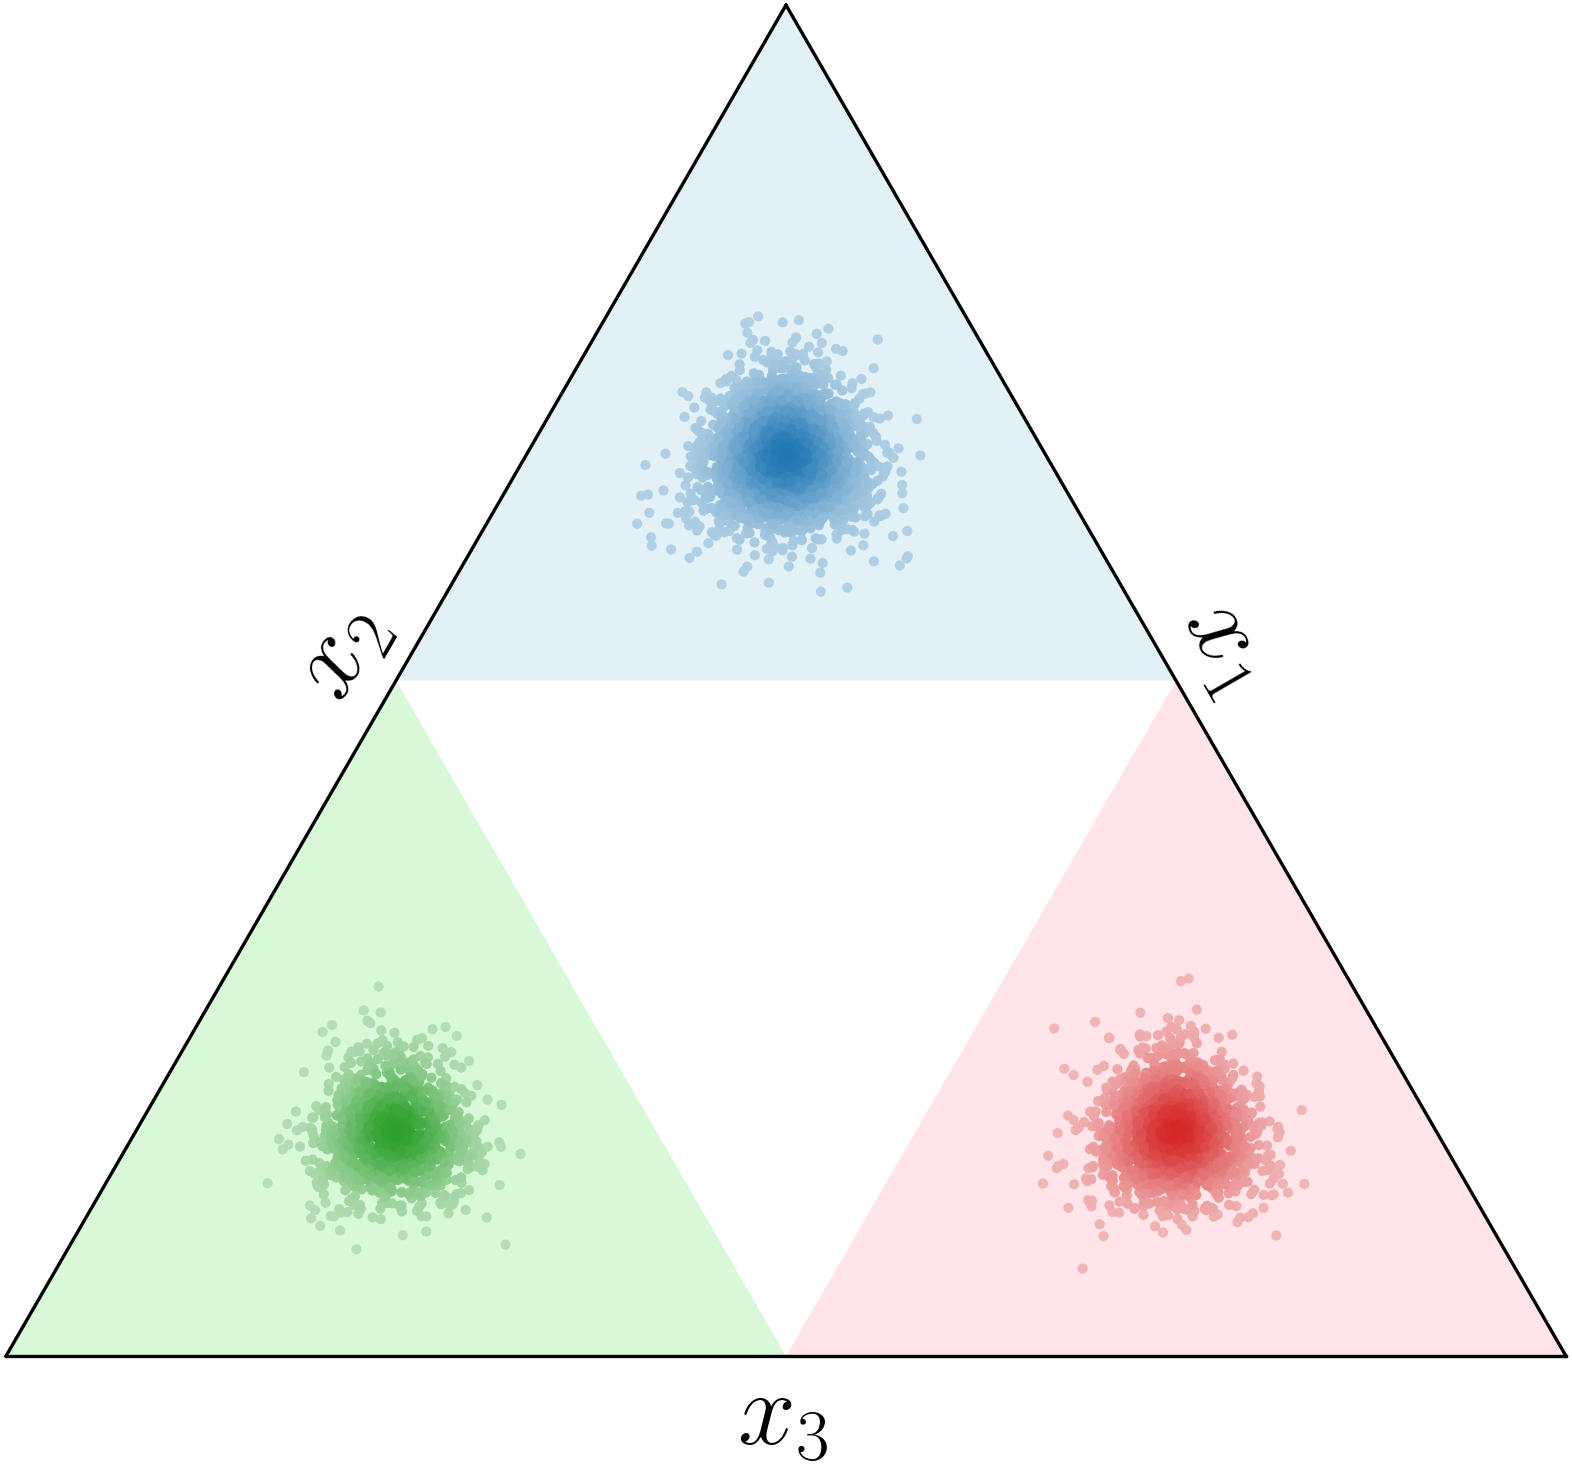
\includegraphics[width=\linewidth]{figs/paper3/lambd_0.5.png}
        \caption*{$\lambda=\tfrac{1}{2}$}
    \end{subfigure}
    \begin{subfigure}{0.3\linewidth}
        \centering
        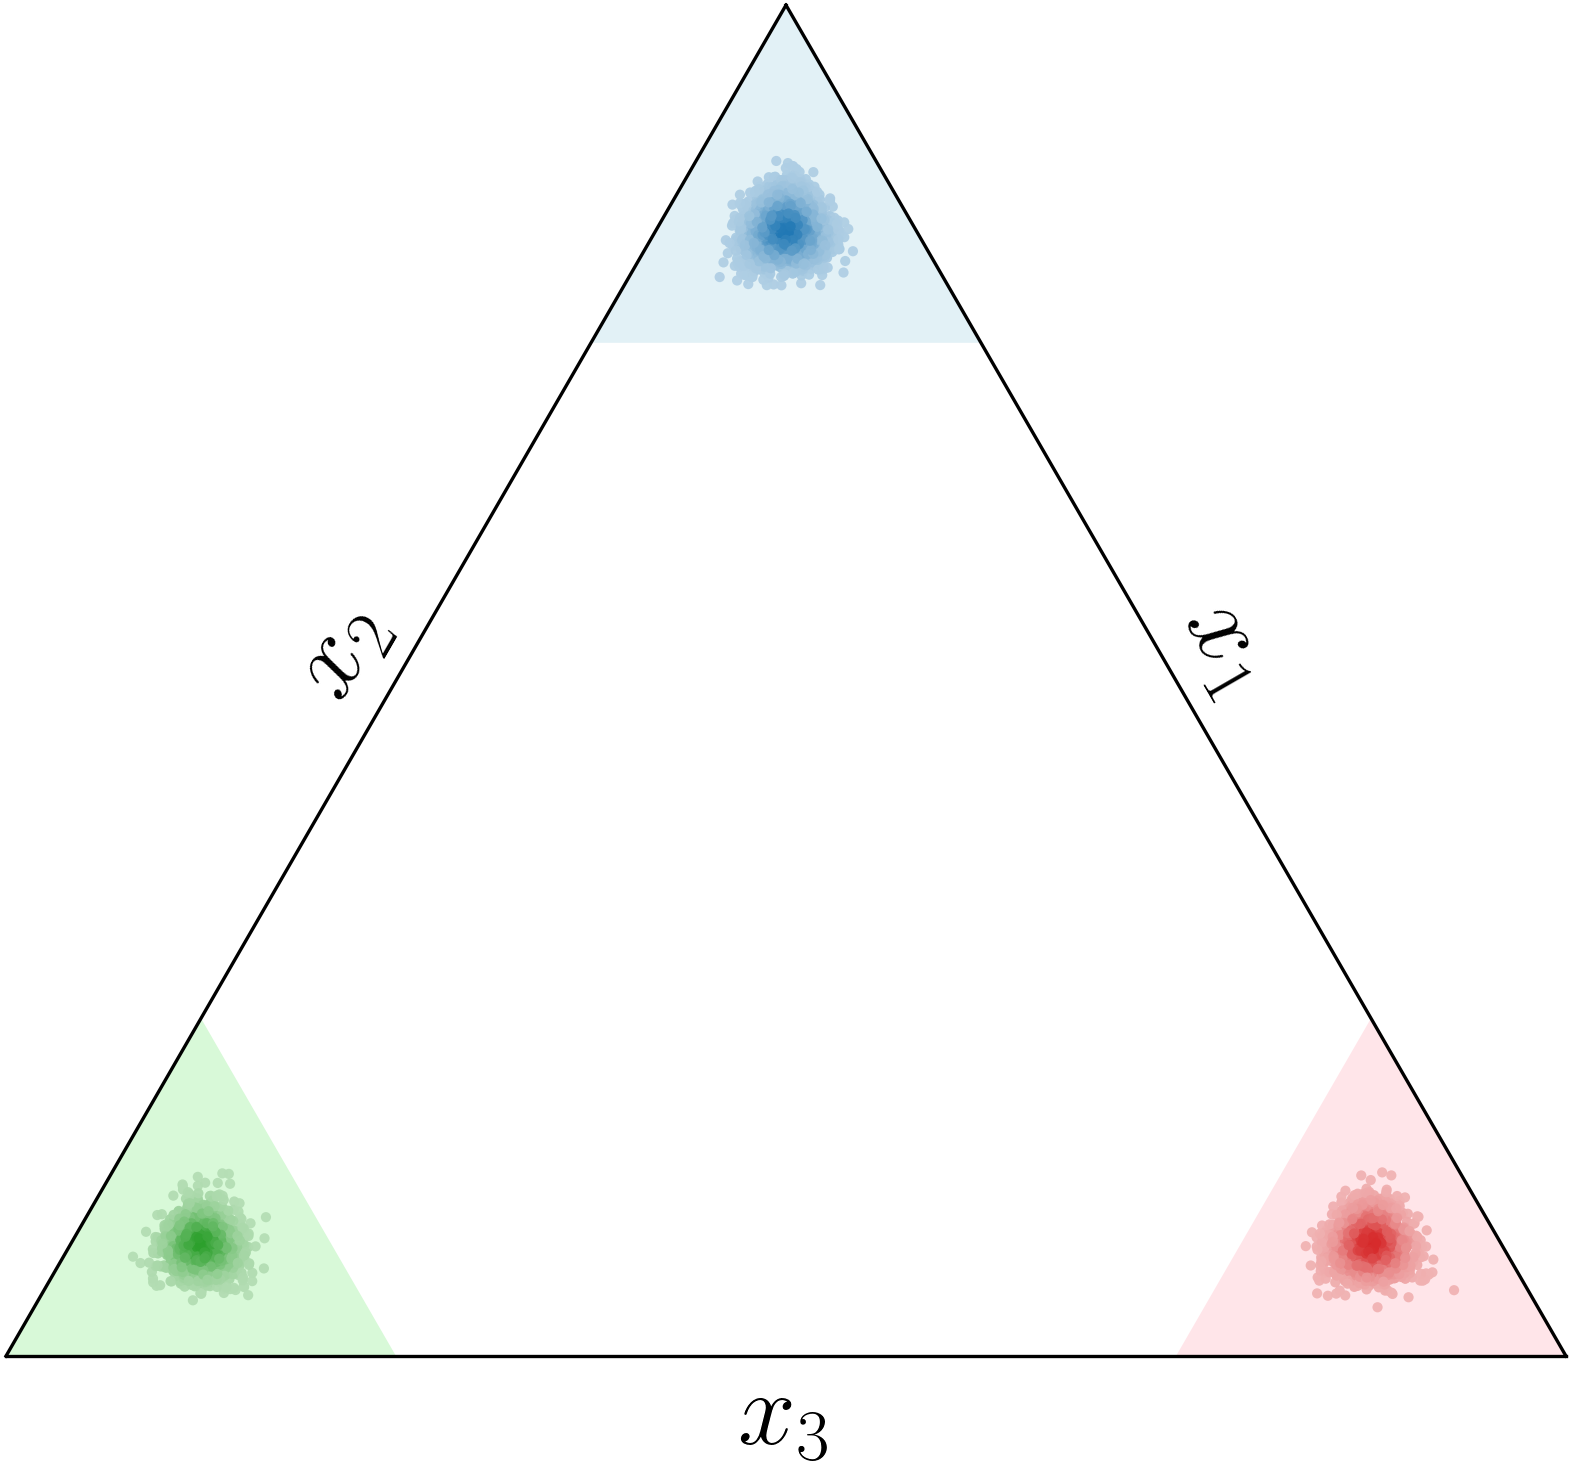
\includegraphics[width=\linewidth]{figs/paper3/lambd_0.75.png}
        \caption*{$\lambda=\tfrac{3}{4}$}
    \end{subfigure}
    \caption{Dirichlet interpolation. The $\lambda$ parameter controls the mixture distribution. For $\lambda \ge \tfrac{1}{2}$ the supports do not overlap and we can recover the categories almost surely. Large $\lambda$ unnecessarily concentrates the mass around the simplex borders we want to avoid.  $\lambda=\tfrac{1}{2}$ illustrates  the $\arg\max$ regions by  the different color blocks.
}
    \label{fig:lambda}
\end{figure}


\paragraph{Latent Gaussian interpolation}
In some cases it is more convenient to place the distribution of the noise process directly on Euclidean latent space. We do this by first interpolating in the simplex space, mapping to Euclidean space with the bijection and adding noise there. For each class $k$, define the interpolated point
\begin{equation}
    \boldsymbol\mu^{(k)} := \lambda\,\boldsymbol e_k + (1-\lambda)\,\tfrac{1}{K}\boldsymbol 1 \in \mathring\Delta^{D},
\qquad \lambda\in(0,1),
\end{equation}
and map it to the latent mean vector $\boldsymbol{m}^{(k)} = \varphi(\boldsymbol\mu^{(k)})$. We then define the latent Gaussian interpolation
\begin{equation}
\boxed{
\boldsymbol z\mid c=k
\sim
\mathcal N\!\bigl( \boldsymbol{m}^{(k)},\,\sigma^2\mathbf I_D\bigr).
}
\label{eq:lik}
\end{equation}

The discrete labels are distributed as $c\sim\mathrm{Cat}(\pi_1,\dots,\pi_K)$, where the class-probability vector $\boldsymbol{\pi}\in\Delta^D$ is unknown.
The distribution in latent space is a Gaussian mixture (see Figure~\ref{fig:likelihood}) centered at $\boldsymbol m^{(k)}$. This can be seen by marginalizing over the classes,
\begin{equation*}
\begin{aligned}
p(\boldsymbol z) = \sum_{k=1}^K p(c=k)\, p(\boldsymbol z\mid c=k) = \sum_{k=1}^K \pi_k\,\mathcal N\!\bigl(\boldsymbol z\mid \boldsymbol m^{(k)},\,\sigma^2\mathbf I_D\bigr).
\end{aligned}
\end{equation*}
\begin{figure}
    \centering
    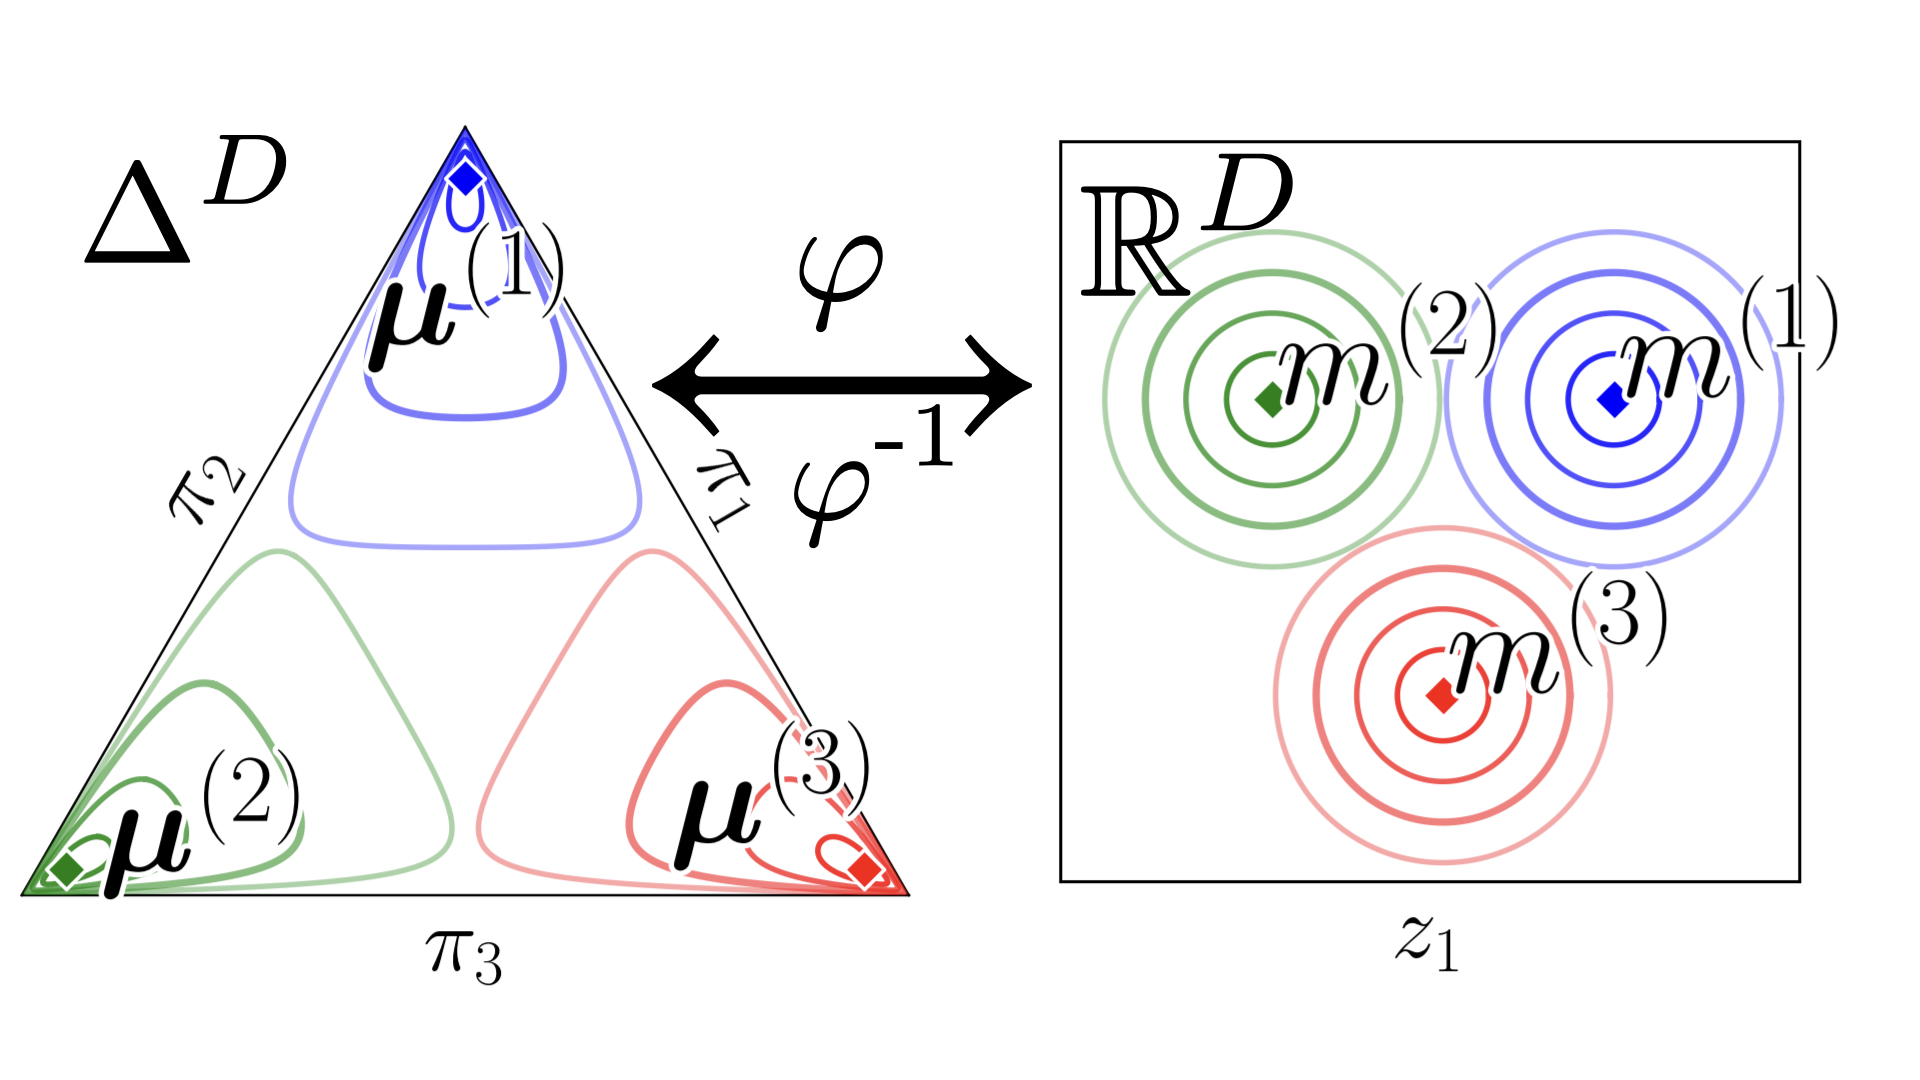
\includegraphics[width=0.8\linewidth]{figs/paper4/lik.001.jpeg}
    \caption{The likelihood of observing classes $1$, $2$, or $3$ is a Gaussian mixture with  modes at $\boldsymbol m^{(k)}=\varphi(\boldsymbol\mu^{(k)})$ in Euclidean space (right), which induces a pushforward likelihood on the simplex (left). The figure shows the likelihood for class probabilities $\boldsymbol{\pi} = (1/3,1/3,1/3)$.}
    \label{fig:likelihood}
\end{figure}

The design choice is the value $\sigma^2$. This parameter controls the overlap between the components, and we can relate this overlap to the probability of the stochastic interpolation being in the incorrect $\arg\max$ region. The key insight is the isometry: distances in the latent space equal distances in the open simplex
\[
\delta := d_A\!\bigl(\boldsymbol\mu^{(k)},\boldsymbol\mu^{(\ell)}\bigr) = \|\boldsymbol m^{(k)}-\boldsymbol m^{(\ell)}\|_2,\qquad k\neq \ell,
\]
and the probability of misclassification is the probability of being closer in Euclidean distance to $\boldsymbol m^{(j)}$ than to the correct mode $\boldsymbol m^{(k)}$.
Proposition~\ref{prop:sigma_bound} gives a sufficient condition on $\sigma$ to make the probability of leaving the correct region (misclassification) smaller than a prescribed tolerance $\varepsilon$.


\begin{proposition}[Proposition 1, Paper IV]\label{prop:sigma_bound}
Let $K\ge 2$.  Define, for each class $k\in\{1,\dots,K\}$,
\[
 \boldsymbol m^{(k)} := \varphi\!\bigl(\boldsymbol\mu^{(k)}\bigr)\in\mathbb R^{D}, \quad \delta := \|\boldsymbol m^{(k)}-\boldsymbol m^{(\ell)}\|_2, \quad k\neq \ell,
\]
where $\delta$ is the Aitchison distance between the class centers on the simplex by the ILR isometry.
Let $\mathcal V_k:=\{\boldsymbol z\in\mathbb R^{D}:\|\boldsymbol z-\boldsymbol m^{(k)}\|_2\le \|\boldsymbol z-\boldsymbol m^{(\ell)}\|_2\ \forall \ell\}$.
For any $\varepsilon\in(0,1)$, if
\begin{equation}\label{eq:sigma_bound}
\sigma \;\le\; \frac{\delta}{2\; z_{1-\varepsilon/D}},
\qquad z_{q}:=\Phi^{-1}(q),
\end{equation}
where $\Phi$ is the standard normal CDF,
then for every $\boldsymbol{x}\in \mathring\Delta^D$ and every $k\in\{1,..,K\}$, the probability of miss-classification is bounded by $\varepsilon$,
\[
\mathbb P\!\big(\boldsymbol Z\notin \mathcal V_k \,\big|\, C=k,\boldsymbol{x}\big)\;\le\;\varepsilon,
\]
where $C$ denotes the class label and $\boldsymbol Z\sim\mathcal N(\boldsymbol m^{(k)},\sigma^2\mathbf I_D)$.
\end{proposition}





\section{Case Study III: Categorical Flow Matching}
This case study combines Flow Matching introduced in Section~\ref{sec:discrete_data} with the simplex-to-Euclidean bijections and the stochastic interpolations developed in this chapter. The proposed method is Simplex-to-Euclidean Flow Matching, where the generative model is trained on Euclidean coordinates but produces samples on the simplex.

Unlike Statistical Flow Matching \citep{Cheng2024, Davis2024}, which uses the Fisher geometry of the simplex and performs Riemannian flow matching on the sphere, our method does not learn the flow on a curved manifold. Instead, we map the problem to $\mathbb{R}^D$, where Euclidean conditional flow matching is applied. This removes the need for Riemannian operations such as the exponential and logarithm maps during training and sampling.

\paragraph{Simplex-to-Euclidean Flow Matching (FM-$\mathring\Delta$)}
Algorithm~\ref{alg:train} details the training procedure of our method. If the data is in the interior of the simplex then the bijection is enough, but if the data is discrete on the boundary, we first use the stochastic interpolation to move the data to the interior and then apply the bijection $\varphi$ and train the Euclidean flow. During sampling the $\arg\max$ converts the continuous process to discrete predictions.
Sampling is done with the procedure specified in Algorithm~\ref{alg:sample_sfm} with an additional $\arg\max$ operator if the generated data is discrete. Any of the simplex-to-Euclidean bijections can be used within the method, and the accuracy is affected by this choice. These include additive logratio, multiplicative log ratio, stick-breaking, and isometric logratio.
Note that using conditional flow matching is a design choice, the procedure is valid for any continuous Euclidean generative model, for example diffusion models \citep{song2021score, Karras2024}.

\begin{algorithm}
\caption{Training of Simplex-to-Euclidean Flow Matching.}
\label{alg:train}
\begin{algorithmic}[1]
\Require Data $\boldsymbol{c}\!\in\!\Delta^{D}$, weight $\lambda\!\in\!(0,1)$, 
Dirichlet $\alpha>0$, bijection $\varphi$, base $p_0$ (e.g. $\mathcal{N}(\boldsymbol{0},\boldsymbol{I})$), 
coupling $\pi$ (indep. or minibatch OT), isDiscrete
\For{each mini-batch}
  \For{each $\boldsymbol{c}$ in batch}
    \If{isDiscrete}
      \State Sample $\boldsymbol{\varepsilon}\!\sim\!\mathrm{Dir}(\alpha,..,\alpha)$
      \State ${\boldsymbol{x}} \gets \lambda \boldsymbol{c}+(1-\lambda)\boldsymbol{\varepsilon}$
    \Else
      \State ${\boldsymbol{x}} \gets \boldsymbol{c}$
    \EndIf
  \EndFor
  \State $\boldsymbol{z}_1 \gets \varphi({\boldsymbol{x}})$ \Comment{Map to Euclidean space.}
  \State Sample $\boldsymbol{z}_0 \sim p_0$; pair $(\boldsymbol{z}_0,\boldsymbol{z}_1)$ via $\pi$
  \State Sample $t\sim \mathrm{Unif}(0,1)$
  \State $\boldsymbol{z}_t\!\gets\!(1-t)\boldsymbol{z}_0+t \boldsymbol{z}_1$, \;
         $\boldsymbol{u}_t\!\gets\!\boldsymbol{z}_1-\boldsymbol{z}_0$
  \State Update $\theta$ by 
  $\min \|\boldsymbol{v}_\theta(\boldsymbol{z}_t,t)-\boldsymbol{u}_t\|^2$ \; (Equation~\ref{eq:cfm_loss})
\EndFor
\end{algorithmic}
\end{algorithm}

Proposition~\ref{prop:cat_prob_tv} justifies the correctness of FM-$\mathring\Delta$ for categorical data, it states that if the learned flow model matches the distribution of the interpolated data with the stochastic interpolation, then the true unknown probabilities are recovered by the model's $\arg\max$ estimations. 


\begin{proposition}[Proposition 1, Paper III] \label{prop:cat_prob_tv}
\textbf{Categorical probabilities bound:}
Let $\lambda \ge \tfrac{1}{2}$ so that the Dirichlet-interpolated mixture
$q_\lambda(\boldsymbol{x})=\sum_{k=1}^{K} \pi_k\, q_\lambda(\boldsymbol{x}\mid \boldsymbol{e}_k)$ 
has a.s. disjoint component supports contained in the strict $\arg\max$ regions
$\mathcal{R}_k := \{ \boldsymbol{x}\in \mathring \Delta^{D} : x_k > x_j\ \forall j\neq k\}.$
For any density $\tilde q$ on $\mathring \Delta^D$ define the induced (generated) categorical probabilities
$\hat \pi_k := \int_{\mathcal{R}_k} \tilde q(\boldsymbol{x})\,d\boldsymbol{x}.$
Then the total variation between the true and generated categorical laws is bounded by the $L^1$ distance between the distributions:
\begin{equation*}
\mathrm{TV}(\boldsymbol{\pi},\hat{ \boldsymbol{\pi}})= \tfrac{1}{2}\sum_{k=1}^{K} | \hat \pi_k - \pi_k |
\;\le\; \tfrac{1}{2}\,\|\tilde q - q_\lambda\|_{1}.
    \end{equation*}
In particular, $\|\tilde q - q_\lambda\|_{1}\to 0$ implies $\hat{\boldsymbol{\pi}} \to \boldsymbol{\pi}$ in total variation, and the $\arg\max$ discretization of $\tilde q$ recovers exactly the true categorical distribution.
\end{proposition}






\subsection*{Empirical evaluation}
We highlight two experiments from Paper~III that illustrate the two parts of the construction. The first considers a density supported on the open simplex, where the role of the bijection and geometry can be seen directly. The second is a language-generation task on discrete data, where the full pipeline including stochastic interpolation is needed. The main comparison methods are LinearFM which uses Euclidean geometry on the simplex itself and Statistical Flow Matching (SFM) \citep{Cheng2024, Davis2024}.

\paragraph{Density on the open simplex}
This experiment considers checkerboard data projected to the open simplex. The data is continuous in $\mathring\Delta^2$, so no interpolation is needed in this comparison. The experiment studies the effect of the geometric representation (simplex, simplex-to-sphere, or simplex-to-Euclidean) and two different choices of bijection (SB or ILR). Figure~\ref{fig:checkboard} shows that our method produces samples that align more closely with the target density than both LinearFM and SFM. In particular, the Euclidean baseline on the simplex and the Fisher-sphere construction produce many more invalid samples near the corners, whereas the simplex-to-Euclidean approach better preserves the structure of the target. Both the isometric logratio and stick-breaking bijections work well, with stick-breaking performing slightly better in this example.
\begin{figure}
    \centering
    \begin{subfigure}[b]{0.4\linewidth}
        \centering
        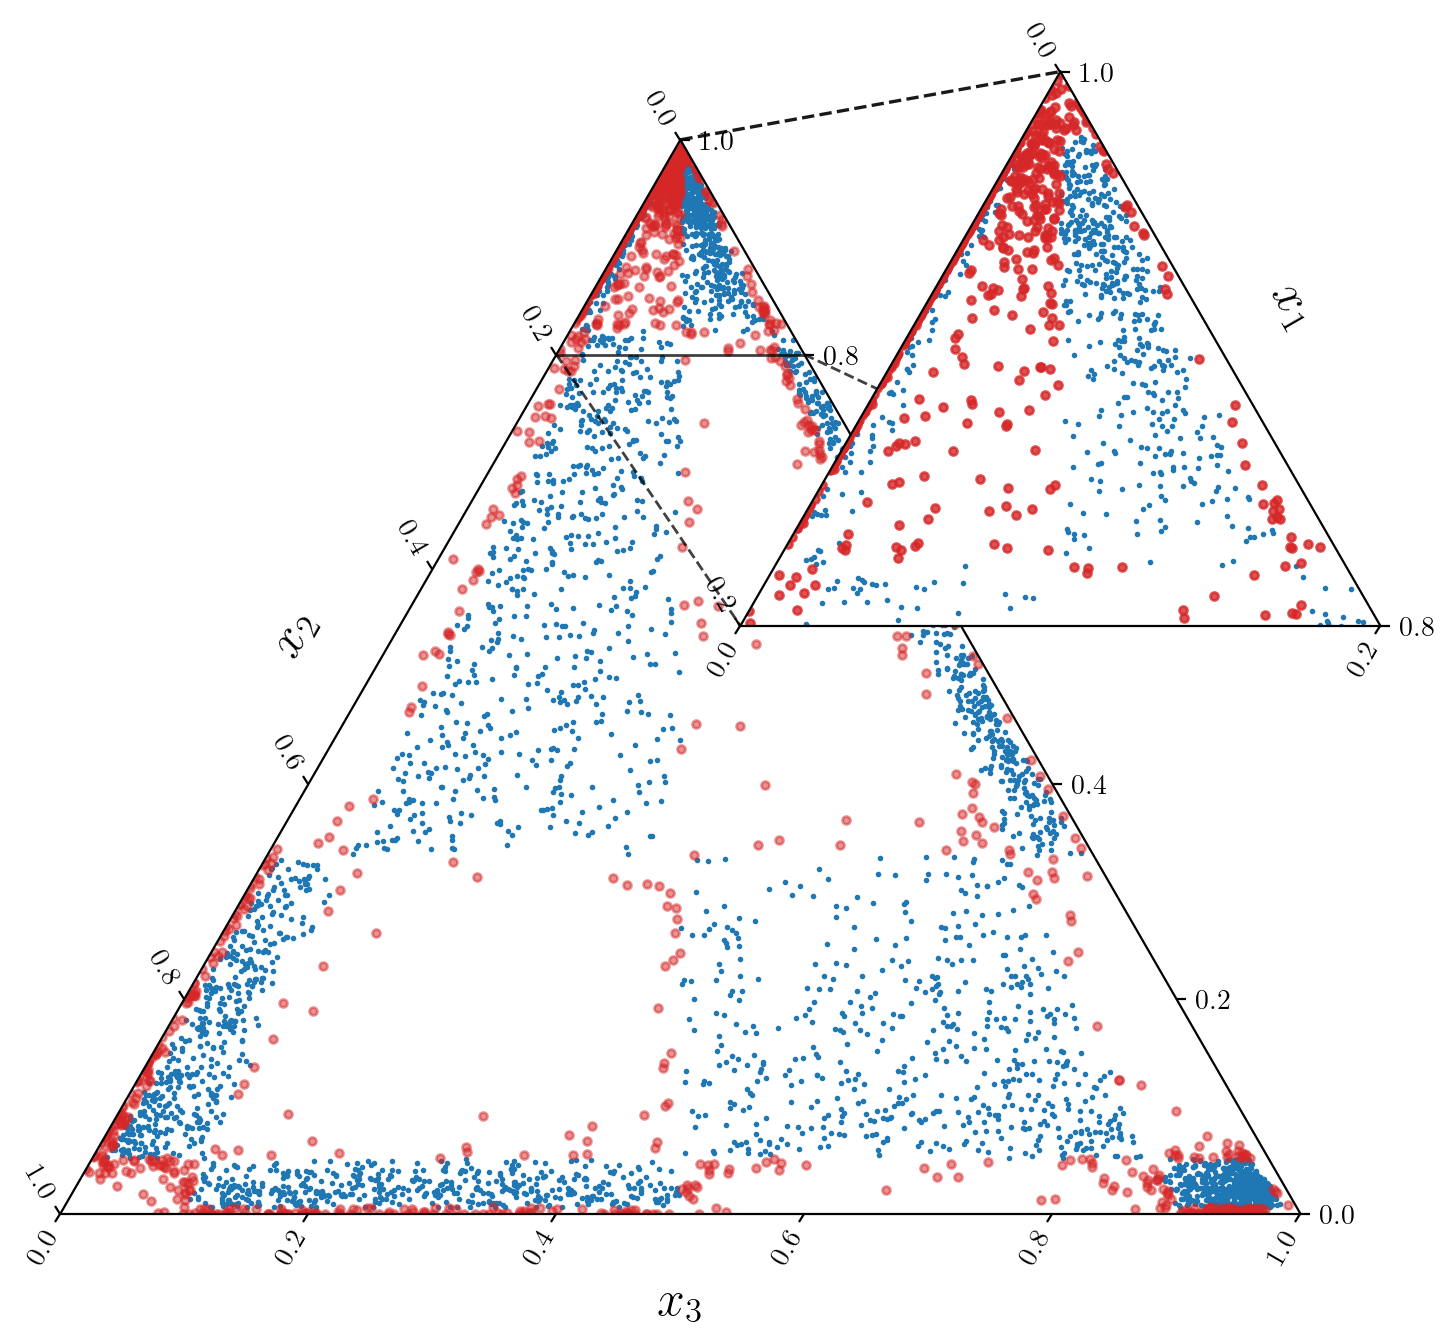
\includegraphics[width=\linewidth]{figs/paper3/checkerboard/linear.png}
        \caption{\footnotesize LinearFM\\ $25.9\%$}
    \end{subfigure}
    \begin{subfigure}[b]{0.4\linewidth}
        \centering
        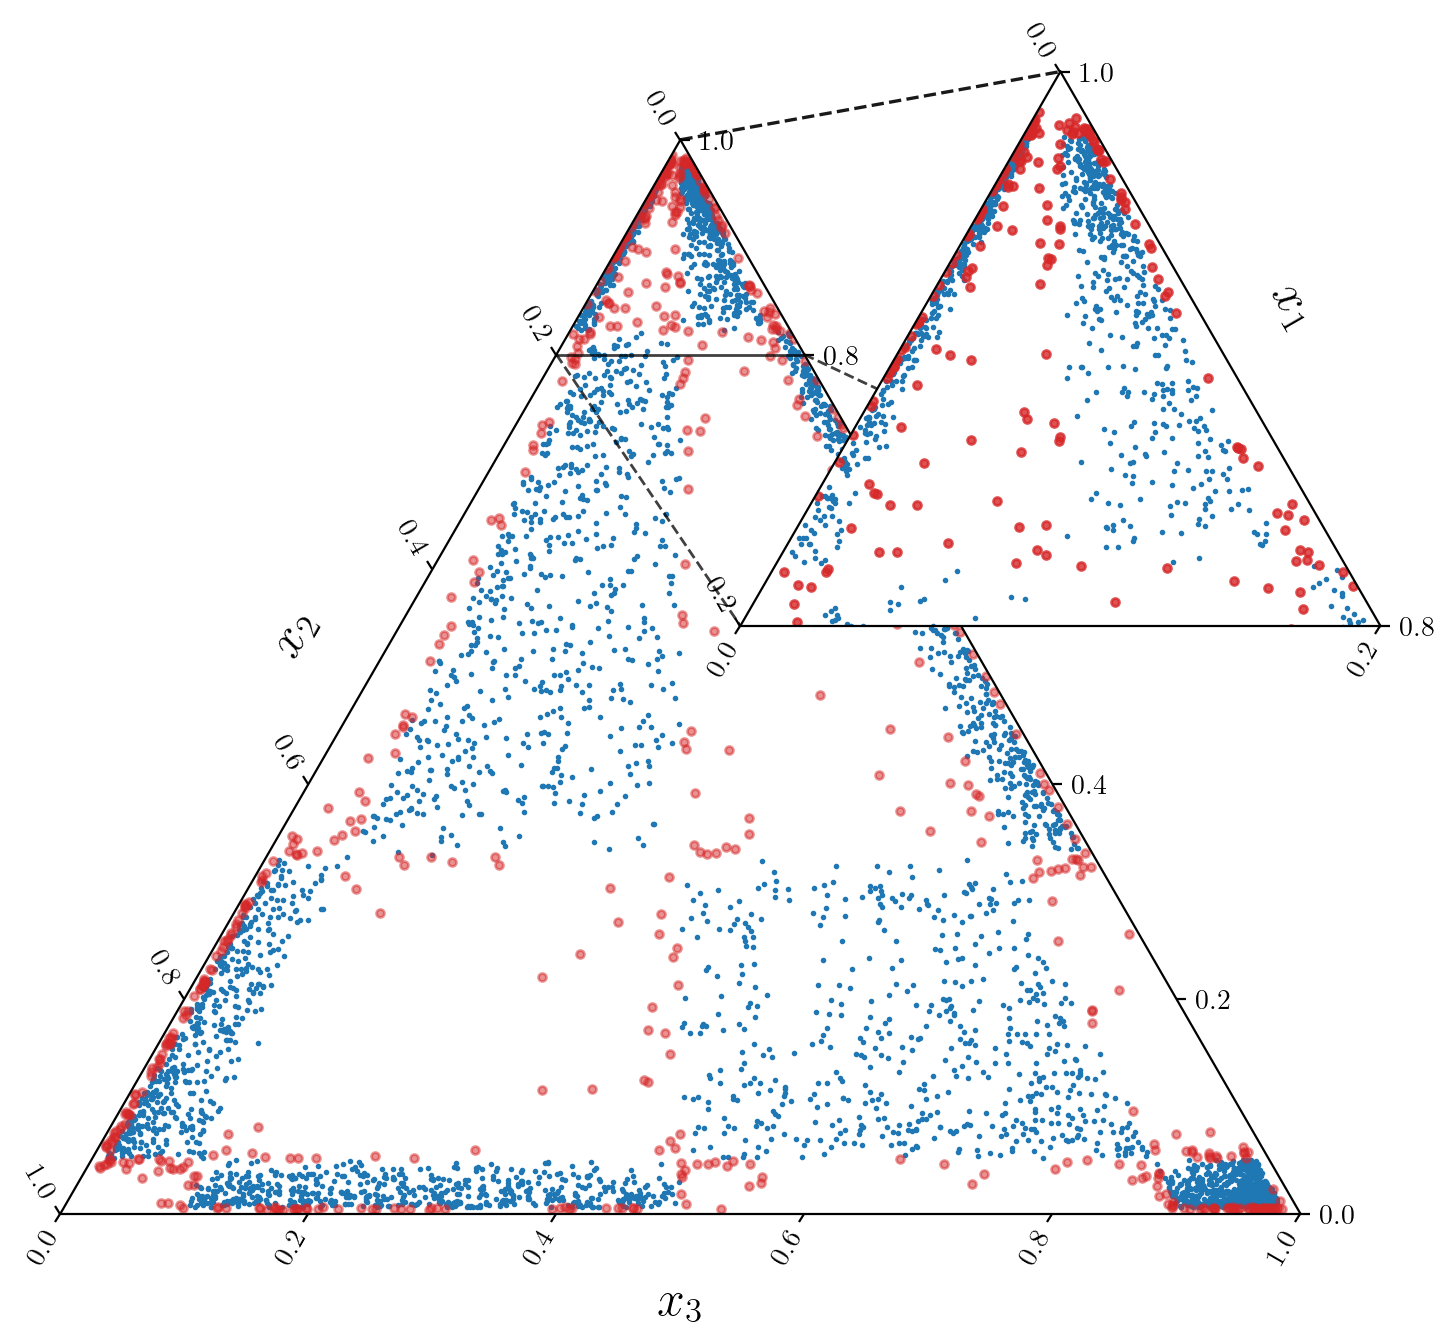
\includegraphics[width=\linewidth]{figs/paper3/checkerboard/sphere.png}
        \caption{\footnotesize SFM\\ $12.9\%$}
    \end{subfigure}
    \begin{subfigure}[b]{0.4\linewidth}
        \centering
        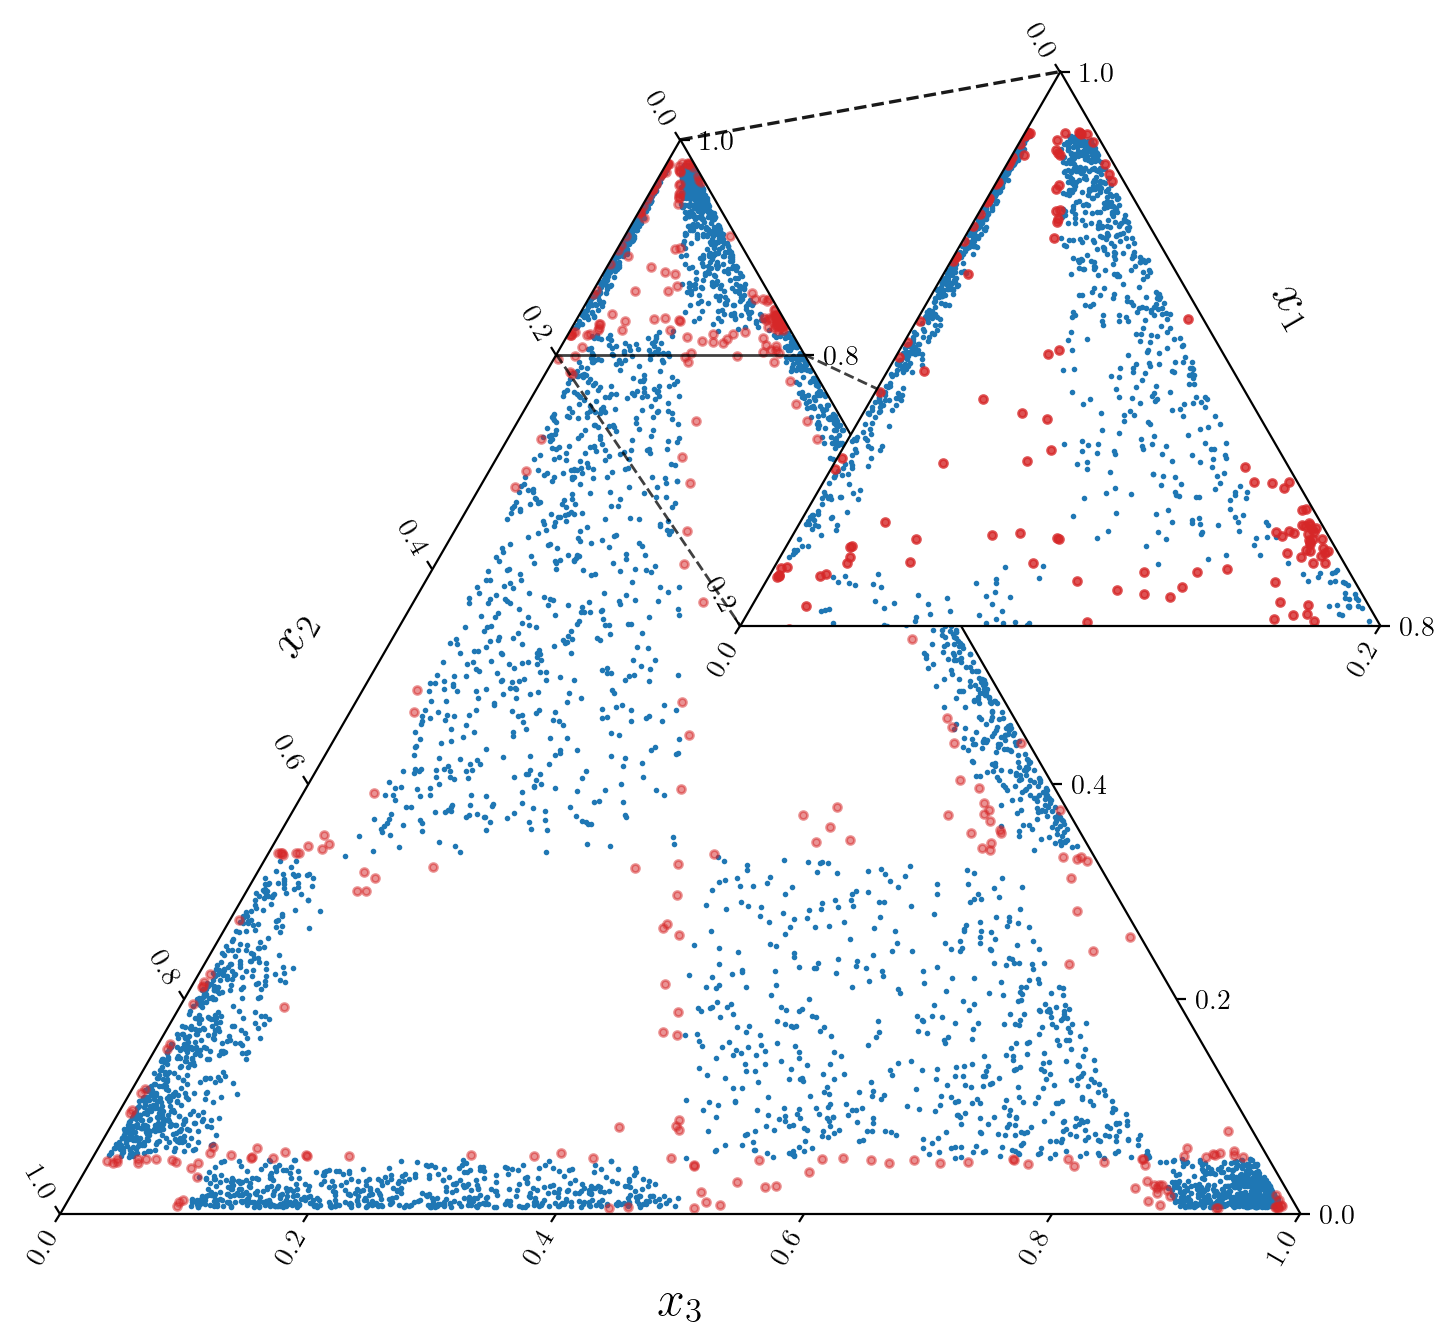
\includegraphics[width=\linewidth]{figs/paper3/checkerboard/ilr.png}
        \caption{ \footnotesize FM-$\mathring\Delta$(ILR)\\ $6.8 \%$}
    \end{subfigure}
    \begin{subfigure}[b]{0.4\linewidth}
        \centering
        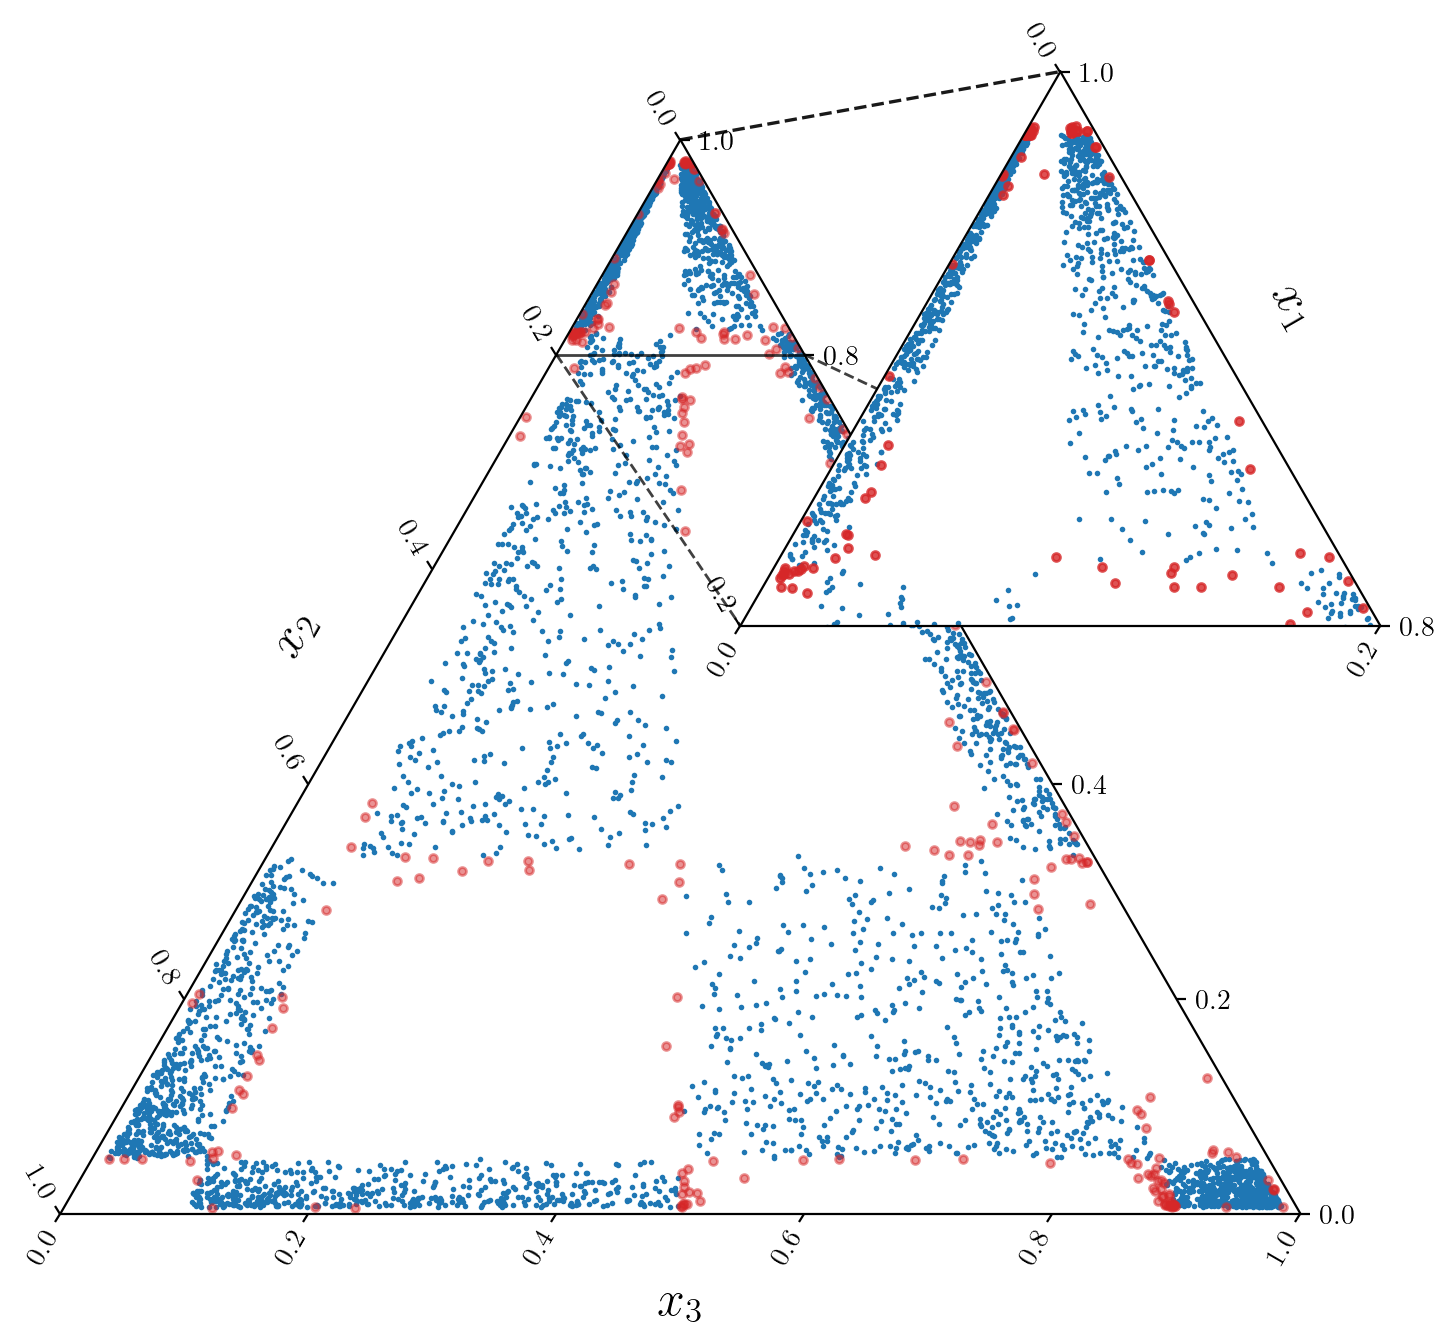
\includegraphics[width=\linewidth]{figs/paper3/checkerboard/sb.png}
        \caption{\footnotesize FM-$\mathring\Delta$(SB)\\ $5.4 \%$}
    \end{subfigure}
    \caption{Samples from Checkerboard on the simplex. Red points indicate samples not aligned with the true density ($\%$ indicated in caption). The zoomed area shows the top region $x_1\geq \tfrac{4}{5}$, emphasizing the differences. }
    \label{fig:checkboard}
\end{figure}

\paragraph{Language generation}
We consider the Text8 dataset \citep{Mahoney2011}, which consists of $K=27$ categories: $26$ letters and the space character, split into random chunks of size $256$. This task illustrates the full discrete-data setting, and we rely on Dirichlet interpolation to move the data to the open simplex, followed by a Euclidean flow model in latent coordinates. We use an auto-regressive model to evaluate the NLL and compute the entropy \citep{Wang2021}; the NLL should be low and the entropy over generated data should be close to the entropy of the test data.
Table~\ref{tab:text8} shows the NLL, entropy, and difference in entropy. It shows that our method is the most competitive among the continuous approaches and improves over LinearFM and SFM. However, the best overall result is obtained by the discrete-state diffusion model SEDD \citep{Lou2024}. SEDD is a discrete diffusion model that operates directly in the discrete space. At the time of submission of our method there was still a gap between latent continuous models and discrete diffusion models, which has been closing recently \citep{lee2026flow}. The outcome is that Simplex-to-Euclidean Flow Matching is a strong continuous baseline, even if it does not fully close the gap to the best discrete-state models.





\begin{table}[t]
\centering
\caption{Text8: NLL and Entropy on the GPT-J-6B model. The baseline results are taken from the respective papers.}
\label{tab:text8}
\begin{tabular}{cllccc}
\cline{2-5}
 & \textbf{Model} & \textbf{NLL $\downarrow$} & \textbf{Entropy} & \textbf{Diff} \\
\cline{2-5}
\multirow{6}{*}{\rotatebox[origin=c]{90}{{\textbf{Discrete}}}}
 & MDLM            & 6.76 & 7.55 & +0.07 \\
 & DFM             & 6.78 & 7.58 & +0.10 \\
 & D3PM            & 6.93 & 7.38 & -0.10 \\
 & SEDD   & \textbf{6.49} & 7.17 & -0.31 \\
 & MultiFlow       & 6.73 & 7.39 & -0.09 \\
\cline{2-5}
\multirow{8}{*}{\rotatebox[origin=c]{90}{{\textbf{Continuous}}}}
 & LinearFM          & 7.35 & 7.62 & +0.14 \\ 
 & $\alpha$-Flow($\alpha{=}{-}0.5)$  & 7.14 & 7.37 & -0.11 \\
 & $\alpha$-Flow($\alpha{=}0.5$)     & 7.00 & 7.42 & -0.06 \\
 & $\alpha$-Flow($\alpha{=}1$)       & 7.09 & 7.51 & \textbf{+0.03} \\
 & SFM             & 6.85 & 7.38 & -0.10 \\ 
 \cdashline{2-5}
 & FM-$\mathring\Delta$(ILR)         & 6.81 & 7.39 & -0.09 \\
 & FM-$\mathring\Delta$(ILR)w{/}OT   & 6.89 & 7.38 & -0.10 \\
\cline{2-5}
 & Data & 4.10 & 7.48 & 0 \\
\cline{2-5}
\end{tabular}
\end{table}



\section{Case Study IV: Gaussian Process Classification}
This case study uses the isometric logratio and the latent Gaussian interpolation to build a multiclass Gaussian process classifier that is conjugate in latent space. Similar to Case Study III, the idea is to map the simplex-valued problem to Euclidean coordinates and then apply a standard continuous model there, in this case the model is Gaussian process regression. We present the method and show with empirical studies that it is accurate and well-calibrated. 


\paragraph{Isometric Logratio Gaussian Process }
Denote the training data as $\{(\boldsymbol r_i,c_i)\}_{i=1}^N$, where $\boldsymbol r_i$ denotes the regressor and $c_i\in\{1,\dots,K\}$ the class label. The construction uses the ingredients introduced earlier in the chapter. Each label $c_i=k$ is moved to the interior of the simplex with the interpolation
\begin{align*}
\boldsymbol\mu^{(k)}&=\lambda\,\boldsymbol e_k + (1-\lambda)\tfrac{1}{K}\boldsymbol 1, 
\end{align*}
and then mapped to Euclidean space with the ILR bijection (Equation~\ref{eq:ilr}) $\varphi$ giving the latent $\boldsymbol m^{(k)}=\varphi(\boldsymbol\mu^{(k)})$. The latent Gaussian likelihood (Equation~\ref{eq:lik}) together with the misclassification probability bound (Proposition~\ref{prop:sigma_bound}), turns classification into GP regression in $\mathbb{R}^D$. The model is
\begin{equation}
\boxed{
\mathbf f(\cdot) \sim \mathcal{GP}(\mathbf 0, K_{\theta}),
\qquad
\boldsymbol z_i\mid \mathbf f(\boldsymbol r_i) \sim \mathcal N\!\bigl(\mathbf f(\boldsymbol r_i),\,\sigma^2\mathbf I_D\bigr).
}
\end{equation}
Since the prior and the likelihood are Gaussian, the model is conjugate in $\mathbb{R}^D$ and posterior inference is exact in $\mathbb{R}^D$. The model uses $D$ latent processes because of the dimensionality of the space. Compared to Dirichlet-based GP classification (Section~\ref{sec:discrete_data}) it requires one less latent process and removes the need for a distributional approximation in the model construction.

For a new regressor $\boldsymbol{r}_*$, class-probability predictions are obtained from the expected value after mapping back to the simplex with $\varphi^{-1}$. Predictions are estimated with Monte Carlo
\begin{equation}
\begin{aligned}
\mathbb E[\boldsymbol\pi_*\mid \boldsymbol{r}_*,\mathcal D] &\approx
\frac{1}{S}\sum_{s=1}^S \varphi^{-1}\!\bigl(\mathbf f_*^{(s)}\bigr) \\
\mathbf f_*^{(s)}&\sim\mathcal N(\boldsymbol\mu_*,\boldsymbol\Sigma_*).
\end{aligned}
\label{eq:gpilr_pred}
\end{equation}
The method's cubic complexity in the size of the training data limits its scalability. For larger data sizes, Paper~IV studies two inducing-point sparse variants. \emph{Uncollapsed-ILR} is a sparse variational classifier that parametrizes the probabilities as $\boldsymbol{\pi} = \varphi^{-1}(\boldsymbol{z})$; the objective factorizes over observations, which allows for mini-batch optimization \citep{Hensman2015}. \emph{Collapsed-ILR} instead keeps the Gaussian process regression in latent space, which is specified with the Collapsed GP regression approximation (see Equation~\ref{eq:lower_bound_collapsed}). The first variant models the probabilities directly while the second approximates the latent GP regression.

\subsection*{Empirical evaluation}
We highlight two experimental evaluations from Paper~IV. The objective of the experiments is to benchmark our work in terms of accuracy and calibration with respect to the existing literature. 
The first studies exact latent inference on small UCI classification tasks, where the full GP posterior can be computed exactly. The second studies larger UCI classification tasks for which we use inducing-point methods for inference. The most important related comparison method is Dirichlet-based Gaussian process (GPD). We additionally include comparisons against models that achieve posterior conjugacy through data augmentation; these are Logistic softmax (LSM) \citep{Galy2020} and Bijective softmax (BSM) \citep{galyfajou2022latent}. We denote by E-ILR our model with exact latent inference, by C-ILR the sparse Collapsed version, and by U-ILR the sparse Uncollapsed version of our method. In all experiments we select the learning rate, data normalization, $\alpha_\varepsilon$ and $\lambda$ using a validation set, and the kernel parameters are optimized with the marginal log likelihood or its lower bound using the training set. We report classification error, negative log-likelihood (NLL), and expected calibration error (ECE).

\paragraph{Exact UCI regression}
We first evaluate the exact ILR model on three small UCI classification data sets, where cubic-time GP inference is still feasible. Figure~\ref{fig:uci_conjugate} shows that our method and Dirichlet-based GP classification achieve similar error rates, but the ILR model attains lower NLL on two of the three tasks and the lowest ECE on all three. This means that the exact ILR construction is at least as accurate as the main conjugate baseline, while giving slightly more calibrated predictive probabilities. The auxiliary-variable methods are consistently worse in this setting.

\begin{figure}
    \centering
    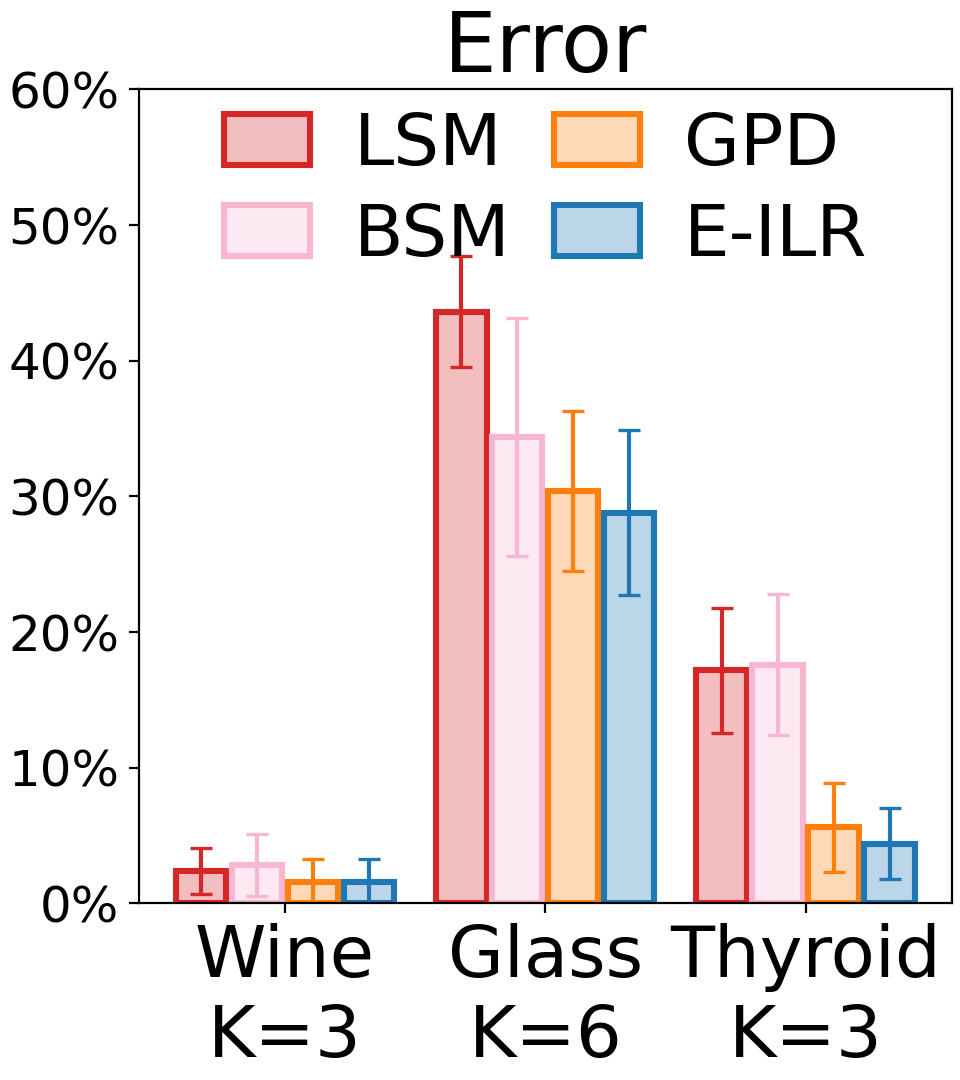
\includegraphics[width=0.3\linewidth]{figs/paper4/uci_conjugate/uci_best_conjugate_per_seed_error.png}
    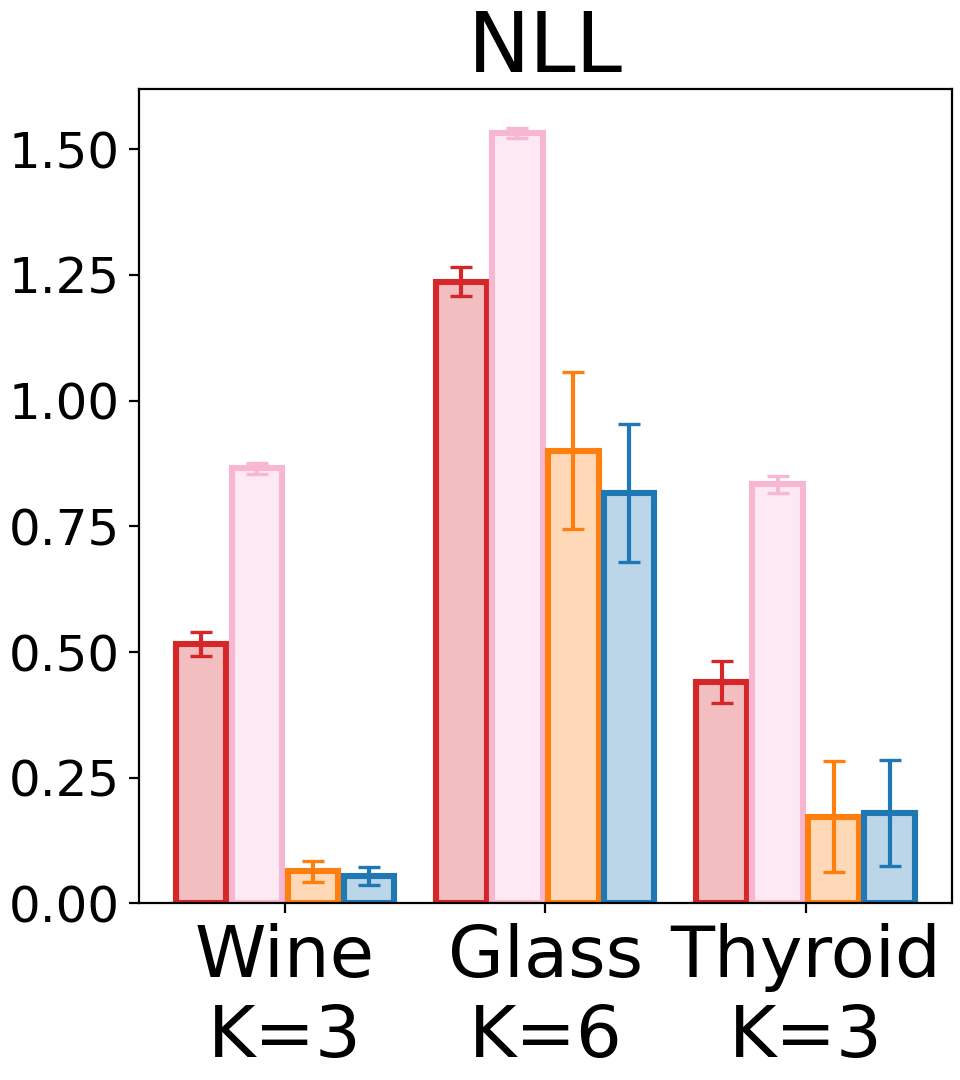
\includegraphics[width=0.3\linewidth]{figs/paper4/uci_conjugate/uci_best_conjugate_per_seed_nll.png}
    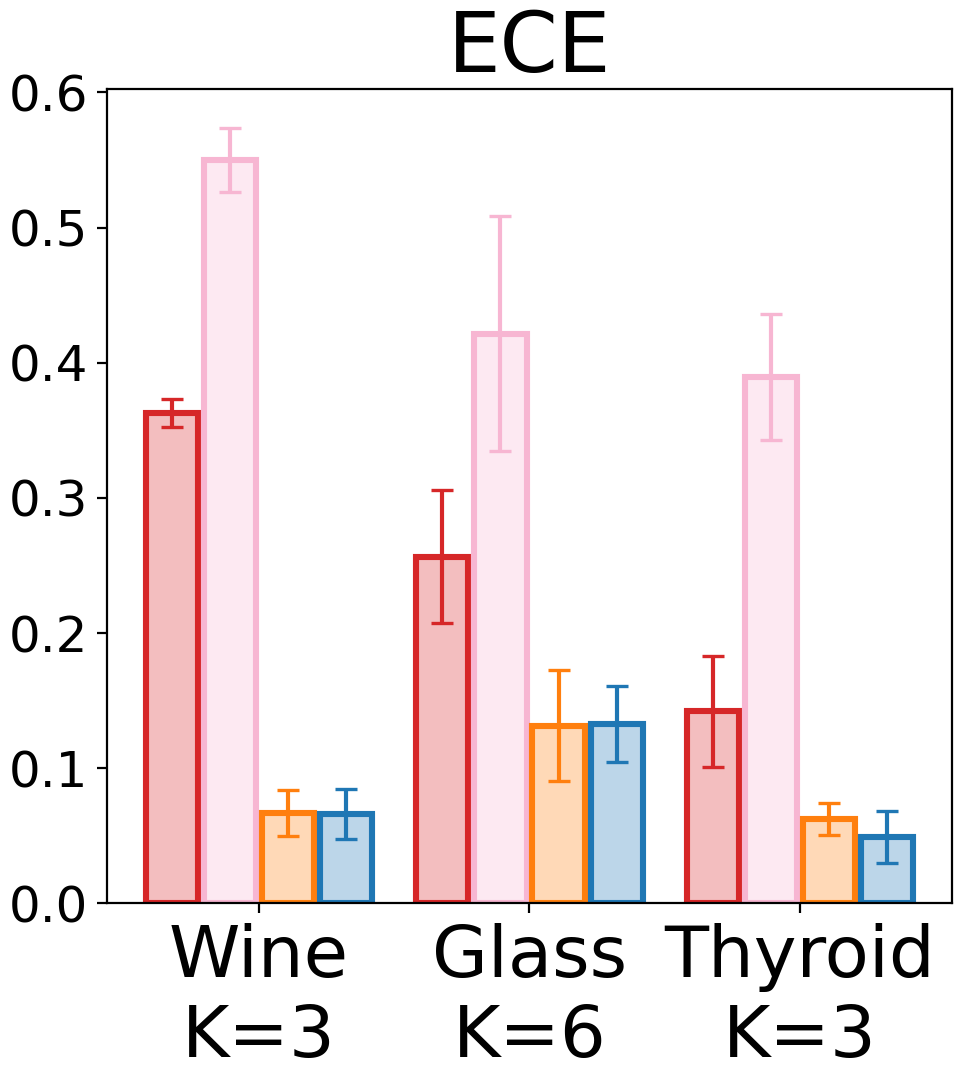
\includegraphics[width=0.3\linewidth]{figs/paper4/uci_conjugate/uci_best_conjugate_per_seed_ece.png}
    \caption{Error, NLL and ECE for UCI datasets in the exact setting.  }
    \label{fig:uci_conjugate}
\end{figure}

\paragraph{Sparse UCI regression}
We next consider seven larger UCI classification benchmarks, where inducing-point approximations are required. Figure~\ref{fig:uci_sparse} summarizes the results. Overall, Collapsed-ILR and sparse Dirichlet GP classification are the strongest methods across the three metrics. The two ILR-based sparse models are competitive with sparse GPD and are often slightly better calibrated. In particular, the ILR-based sparse methods obtain lower ECE on several tasks, and on the \textsc{Letter} data set Uncollapsed-ILR performs better than Collapsed-ILR. The data-augmented softmax baselines struggle here, especially as the number of classes increases. The main conclusion is that the sparse ILR constructions preserve the good calibration of the exact model while scaling to larger problems.


\begin{figure}
    \centering
    \begin{subfigure}[b]{0.7\linewidth}
        \centering
        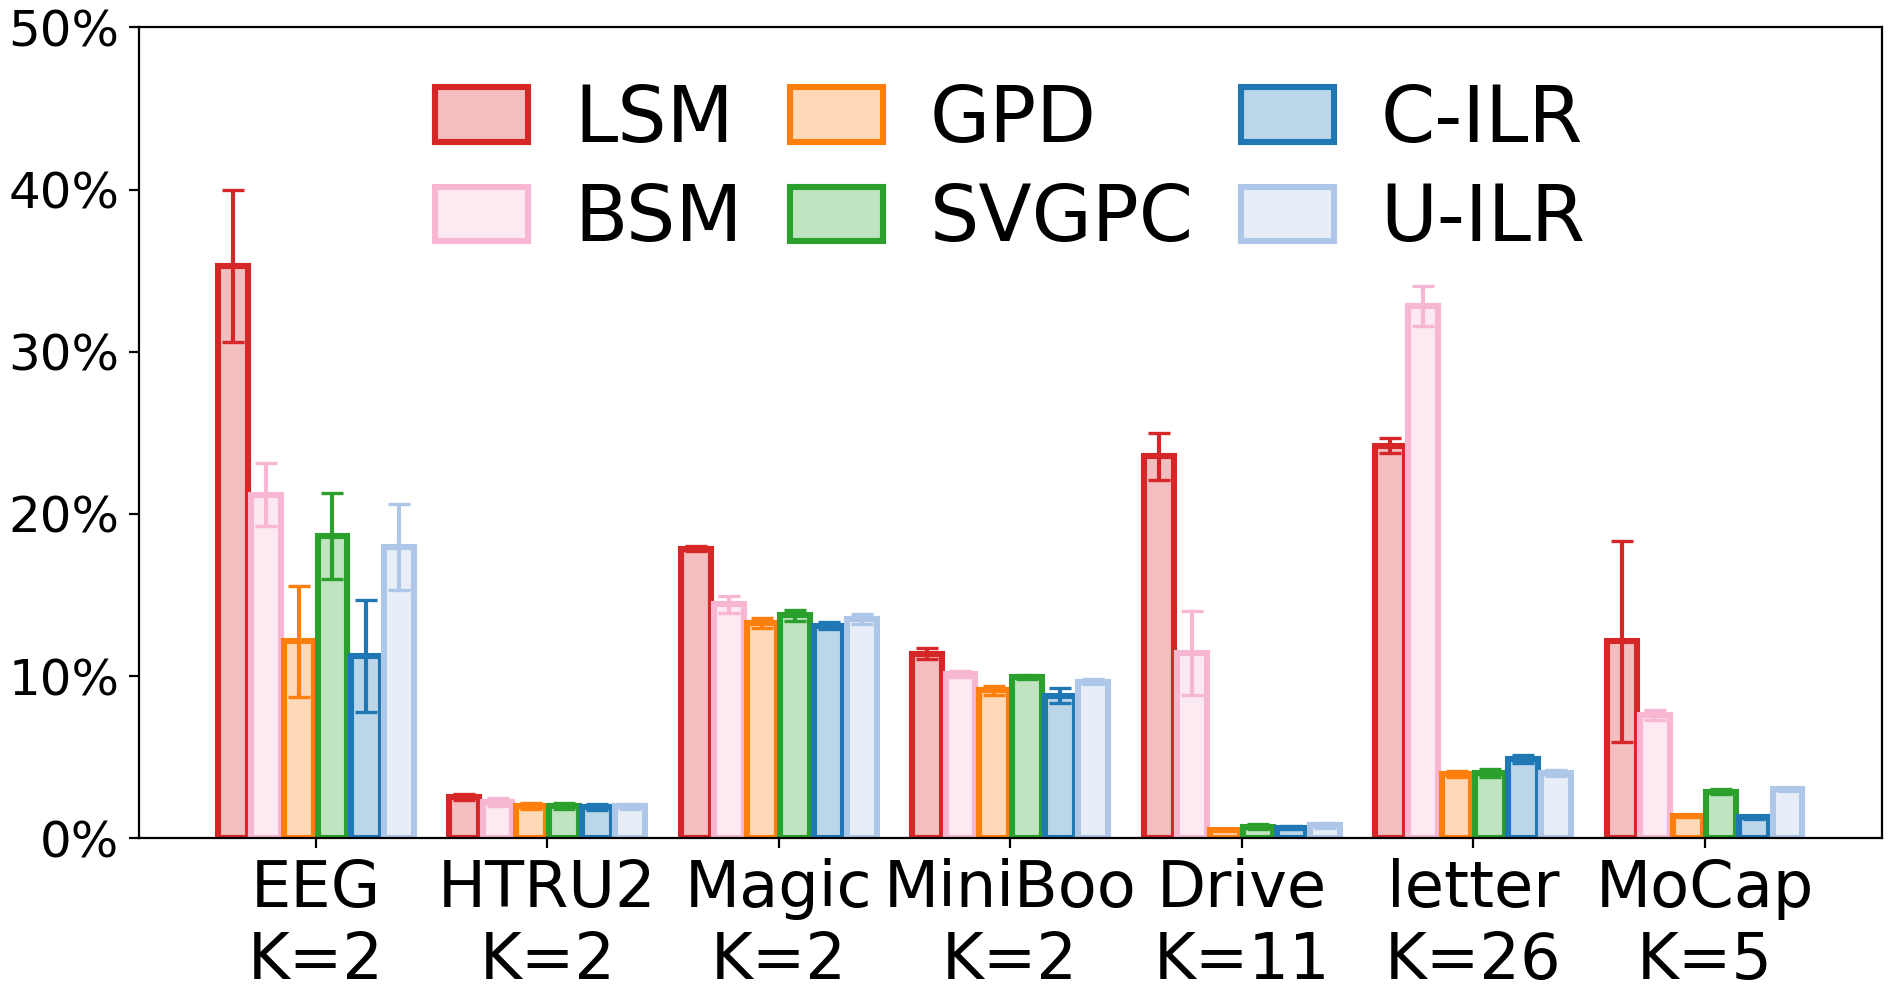
\includegraphics[width=\linewidth]{figs/paper4/uci_sparse/uci_best_sparse_per_seed_error.png}
        \caption{Error rate}
    \end{subfigure}
    \begin{subfigure}[b]{0.7\linewidth}
        \centering
        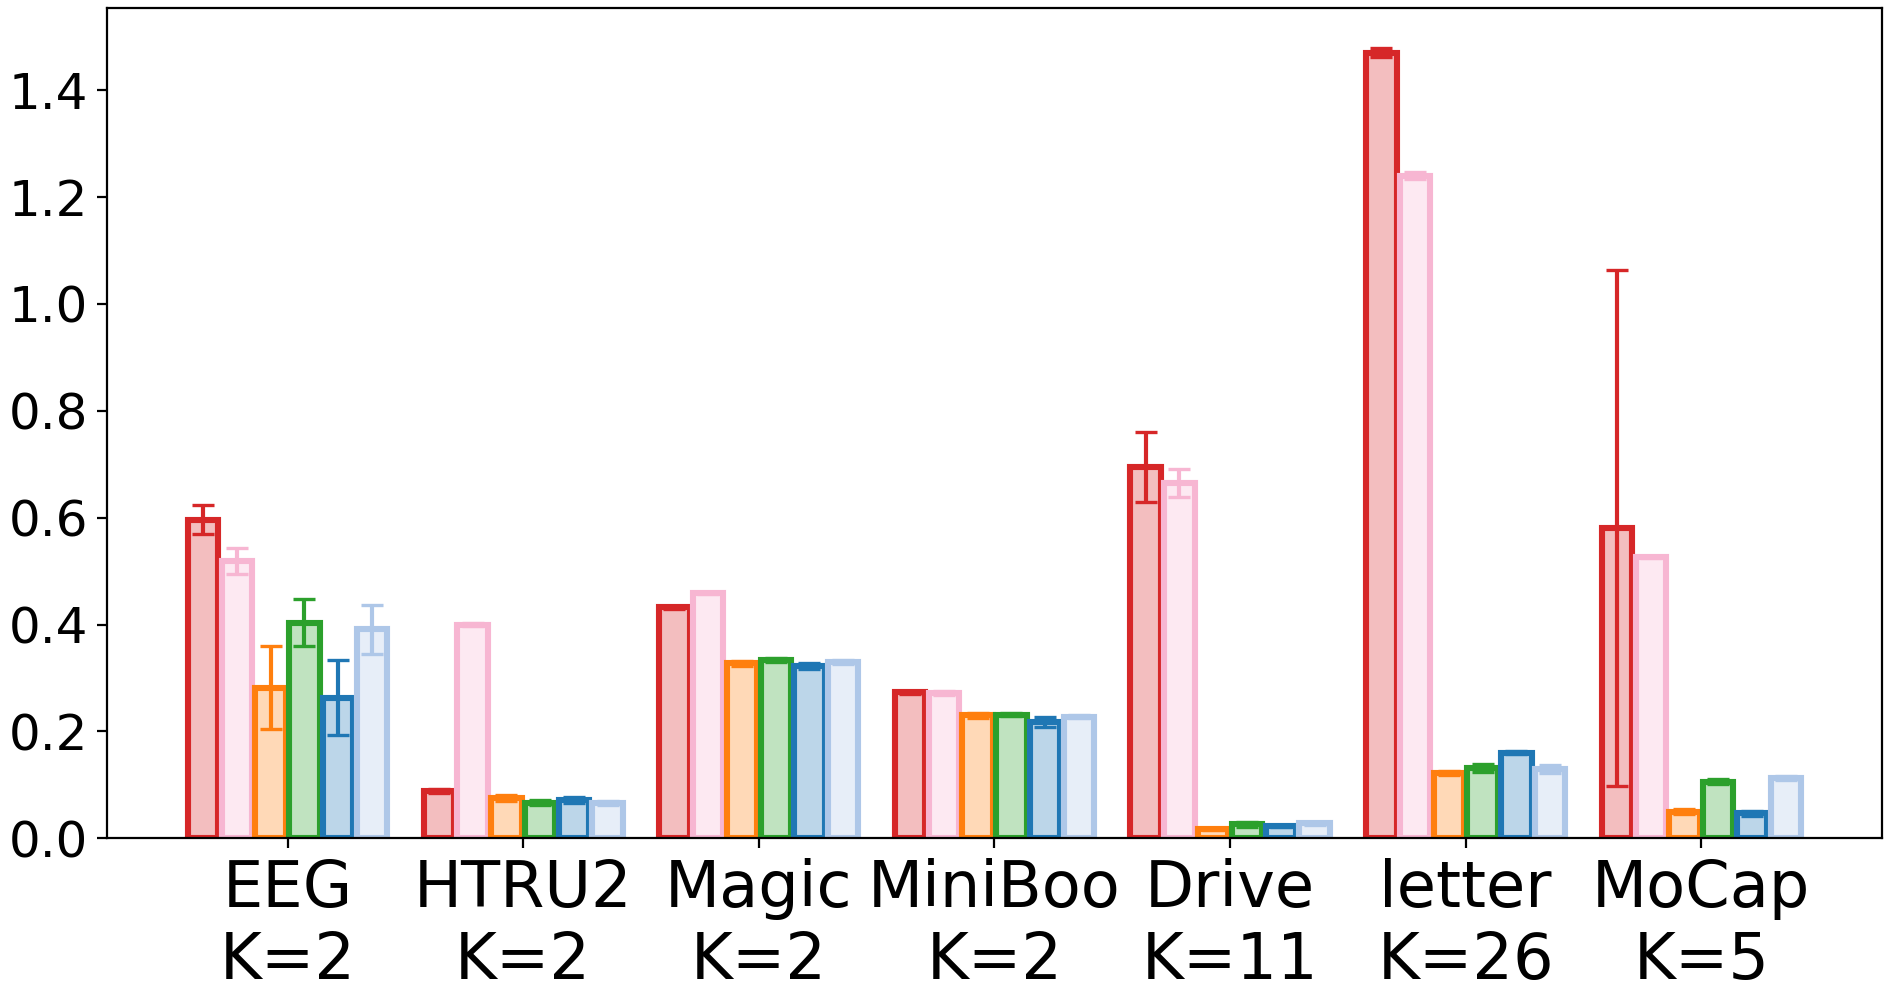
\includegraphics[width=\linewidth]{figs/paper4/uci_sparse/uci_best_sparse_per_seed_nll.png}
        \caption{NLL}
    \end{subfigure}
    \begin{subfigure}[b]{0.7\linewidth}
        \centering
        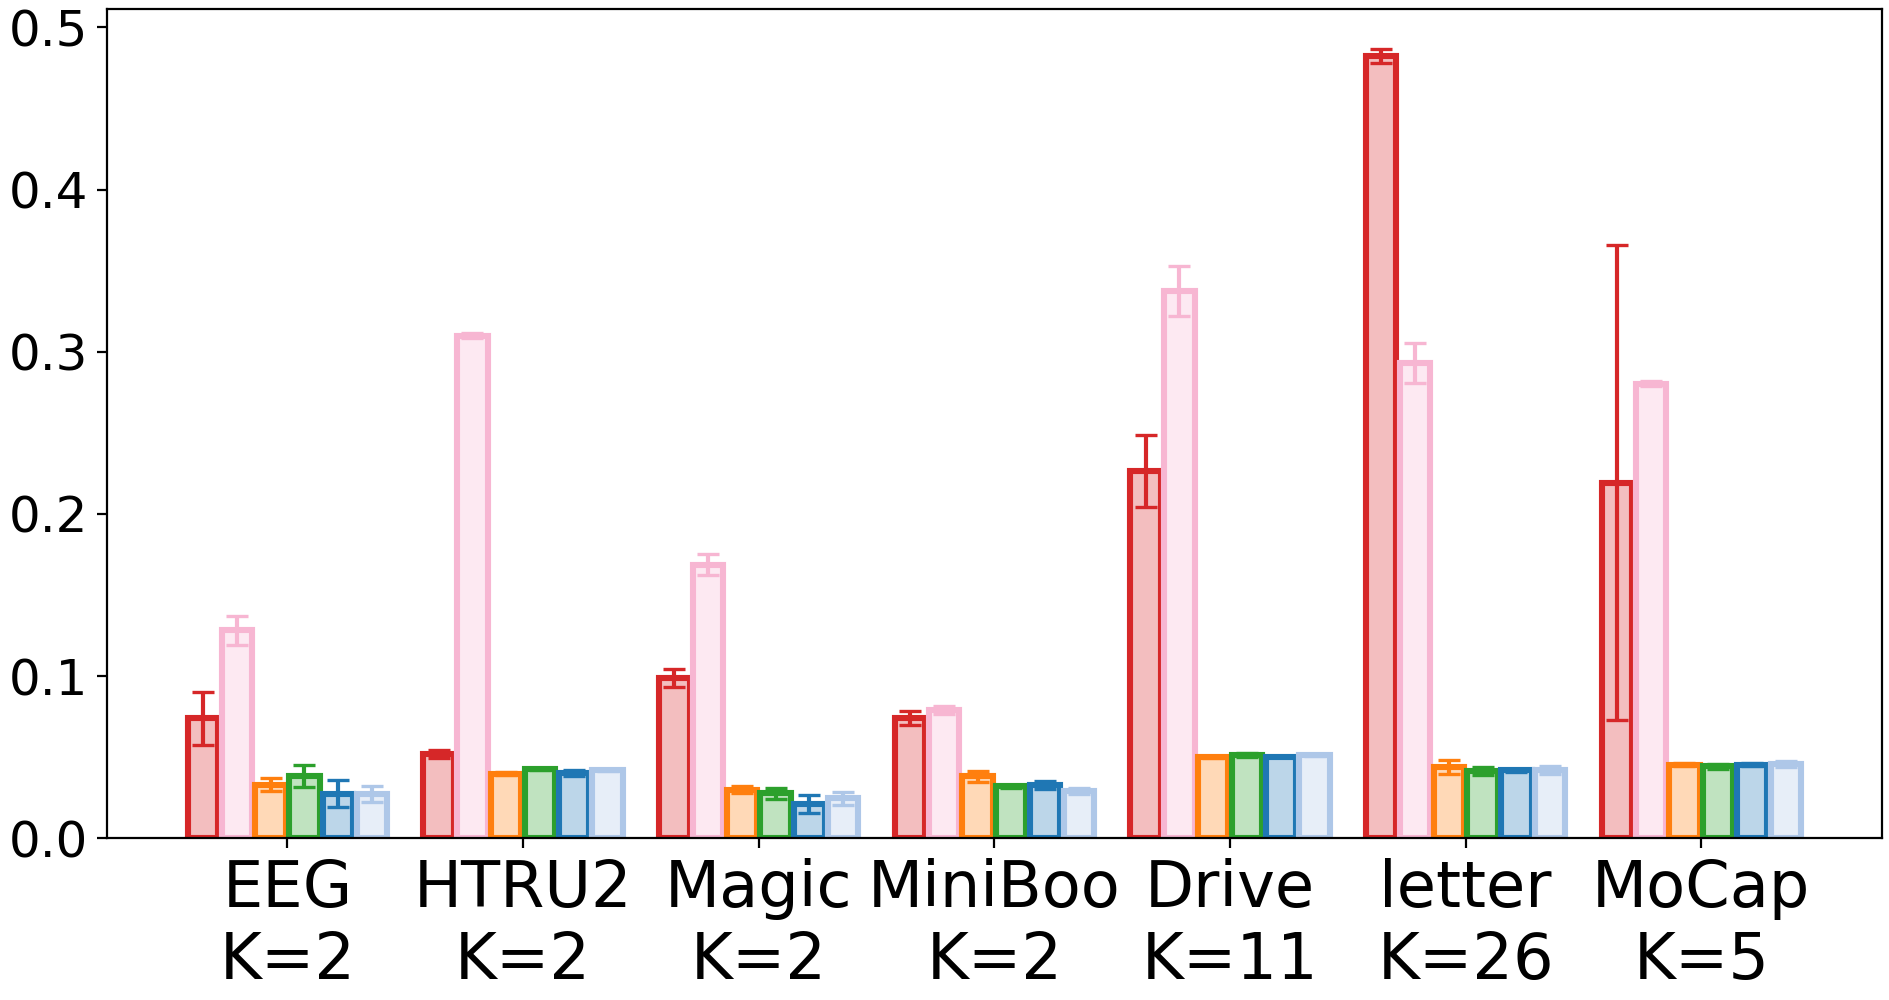
\includegraphics[width=\linewidth]{figs/paper4/uci_sparse/uci_best_sparse_per_seed_ece.png}
        \caption{ECE}
    \end{subfigure}    
    \caption{Sparse models performance on UCI datasets.  }
    \label{fig:uci_sparse}
\end{figure}

\chapter{Conclusion}

\paragraph{Summary of findings}
The findings in this thesis tie to the research questions posed in the introduction. Approximate Bayesian inference can be improved by geometry-aware modeling if the metric is chosen \emph{carefully}. We considered metrics constructed from the target distribution.
Paper~I concluded that the Riemannian Laplace approximation with the Fisher information matches strongly curved targets most accurately in small-dimensional problems.
Paper~II found that the correct choice of metric inside geodesic slice sampling captures curvature. If the target is multimodal, sampling using the inverse metrics improves movement between the modes.

Simplex geometry can be connected to Euclidean representations through stochastic interpolations and simplex-to-Euclidean bijections. Paper~III found that this makes Euclidean generative models applicable to discrete data, while allowing exact recovery of the original category with the $\arg\max$ operation.
Paper~IV showed that the Aitchison geometry together with the latent stochastic interpolation converts the problem into Gaussian process regression, which enables exact latent inference and gives accurate and calibrated predictions.

Overall, the thesis incorporated the geometry of the statistical problem into the method itself, which led to improved accuracy (while making it clear when these gains come at a computational cost) or to a latent simplification of the original problem. Next we give some of the limitations of the methods presented and avenues for future work.

\paragraph{Limitations and Outlook}
The main limitation of Papers I and II is computational complexity: numerical integration is expensive, and each integration step becomes cubic in complexity for the Fisher information metric. Future work can study (i) approximations of the geodesics, for example Taylor approximations \citep{hartmann:2023}, and (ii) amortization of the geodesics, for example geometry-aware variational approximations \citep{chevallier2022exponential}.

A limitation of Paper II is the lack of a guarantee of mode coverage. A more detailed theoretical study could show under which conditions the sampler can generate geodesics that reach other modes.

The main limitation of Paper III is that the method does not scale as well as discrete diffusion with respect to $K$. Recent work has shown that continuous diffusion does scale as well as discrete diffusion with additional improvements \citep{roos2026categorical, lee2026one}. Future work can explore whether training the flow directly with the negative categorical log likelihood (cross entropy) can improve our method in the same way. Another distinction with discrete diffusion is that some of these methods model the score only for a subset of categories \citep{Lou2024}, whereas we model all categories at the same time with the velocity field. It might be that restricting the velocity field to move between a subset of categories or to lower-dimensional projections improves the scalability of our method.

Paper IV shares the limitations of Gaussian process regression: it scales purely with the training data even with sparse approximations. Since our method is compatible with advances in Gaussian process regression, future work can test the scalability of the method on large classification tasks under scalable Gaussian process regression methods \citep{maronas2023efficient}.

The simplex-to-Euclidean bijections and the Aitchison geometry remain largely underutilized in modern machine learning. Other lines of future work include the sampling of densities constrained by a linear system. \citet{Diederen2025} construct a general bijection from convex polytopes to Euclidean space (which uses the ILR map). This can be used as a reparametrization of the target distribution defined on a convex set. In a similar way, high-dimensional categorical distributions can be converted to Euclidean target distributions with our procedure, which can ease sampling \citep{mohanty2026slithering}.

Classification with the softmax function leads to neural collapse \citep{kothapalli2023neural}. Future work can assess whether the ILR map avoids this behavior. This would open up the possibility of computing geodesics in the ILR-latent space, which might lead to improvements in the study of latent geometric representations \citep{yu2025connecting}.


\bibliographystyle{plainnat}
\bibliography{bibtex}

\end{document}
